\documentclass[mathserif]{beamer}
\usepackage{amsmath,amssymb,amsfonts}
\usepackage{mathtools}

%\includeonly{number_electrons}

\usetheme[secheader]{Madrid}
\usecolortheme{ostrich}
\setbeamercovered{transparent=50}
\usepackage{appendixnumberbeamer}

\usepackage[
  labelformat=empty,
  justification=centering,
  font=scriptsize
]{caption}

\usepackage{graphicx}
\graphicspath{{./images/}}
\DeclareGraphicsExtensions{.jpg,.png,.gif}
\usepackage{fancybox}

\usepackage{tikz}
\usetikzlibrary{positioning,calc}
\usetikzlibrary{shapes.geometric,shapes.arrows,shapes.callouts,arrows,decorations.pathmorphing}

\pgfdeclarelayer{background}
\pgfdeclarelayer{below-main}
\pgfdeclarelayer{above-main}
\pgfsetlayers{background,below-main,main,above-main}

\IfFileExists{cache/use_cache.tmp}{
  \usetikzlibrary{external}
  \tikzexternalize
  \tikzsetexternalprefix{cache/}
}

\usepackage{url}

\usepackage[citestyle=authoryear]{biblatex}
\addbibresource{bibliography.bib}

\title[Ultrafast EM]{High Space-Time Resolution\\Transmission Electron Microscopy}
\author{Joel Berger}
\institute[UIC]{Ph.D. Preliminary Examination}
\date{April 26, 2013}

\providecommand{\smallT}[0]{ { \scriptscriptstyle T } }
\providecommand{\dx}[1]{\ensuremath{ \operatorname{d}\!#1 }}
\providecommand{\vf}[0]{\only<presentation>{\vfill}}

\begin{document}

\begin{frame}
  \maketitle
\end{frame}

\begin{frame}{Outline}
  \tableofcontents
\end{frame}

\AtBeginSection{
  \addtocounter{framenumber}{-1}
  \begin{frame}{Outline}
    \tableofcontents[currentsection]
  \end{frame}
}
\AtBeginSubsection{
  \addtocounter{framenumber}{-1}
  \begin{frame}{Outline}
    \tableofcontents[currentsection,currentsubsection]
  \end{frame}
}


\section{Introduction}
\begin{frame}{Motivation --- Galloping Horses}
  \begin{center}
    ``Sallie Gardner at a Gallop'' --- Eadweard Muybridge
    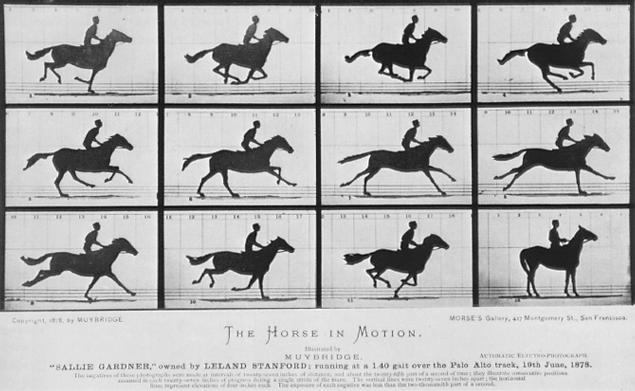
\includegraphics[width=0.75\linewidth]{muybridge_galloping_horse}
  \end{center}
\end{frame}

\begin{frame}{Modern ``Galloping Horses''}
  \begin{center}
    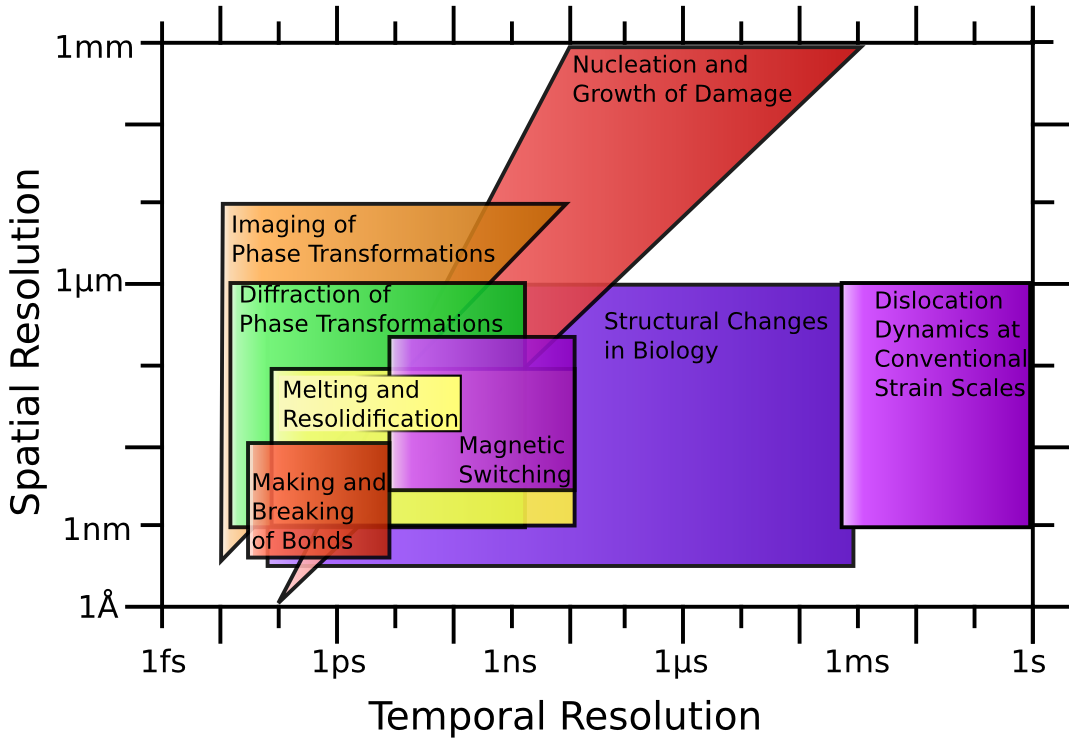
\includegraphics[width=0.85\linewidth]{Resolution}
  \end{center}
\end{frame}

\begin{frame}{Resolutions of TEM and Lasers}
  \begin{columns}	
    \begin{column}{0.49\linewidth}
      Transmission Electron Microscopy (TEM) resolution:
      \begin{itemize}
        \item<2-> JEOL 2010F: 0.19nm
        \item<3-> FEI Titan G2: 0.08nm
        \item<4-> TEAM aberration corrected microscope aims for 0.05nm
        \item<5-> Temporal resolution: video rate (commonly $\sim$30fps)
      \end{itemize}
      \begin{figure}
        \centering
        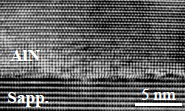
\includegraphics{hrtem}
        \caption{\url{le-csss.asu.edu}}
      \end{figure}
    \end{column}
    \begin{column}{0.49\linewidth}
      Laser resolution:
      \begin{itemize}
        \item<6-> Ultrafast Lasers
        \begin{itemize}
          \item<7-> Ti:Sapphire $\sim 10$fs 
          \item<8-> As short as 80 attosecond
          \item<9-> Limited by optical wavelength
        \end{itemize}
        \item<10-> Near field scanning optical microscopy (NSOM)
        \begin{itemize}
          \item<10-> Uses sub-wavelength apertures
          \item<10-> 2-5nm resolution
          \item<10-> Long scan time
        \end{itemize}
      \end{itemize}
      \begin{figure}
        \centering
        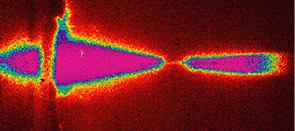
\includegraphics{channel}
        \caption{\url{www.xrimlab.com}}
      \end{figure}
    \end{column}
  \end{columns}
\end{frame}

\begin{frame}{Laser Driven Time-Resolved Electron Microscope}
  \begin{center}
    \begin{tikzpicture}
      \node {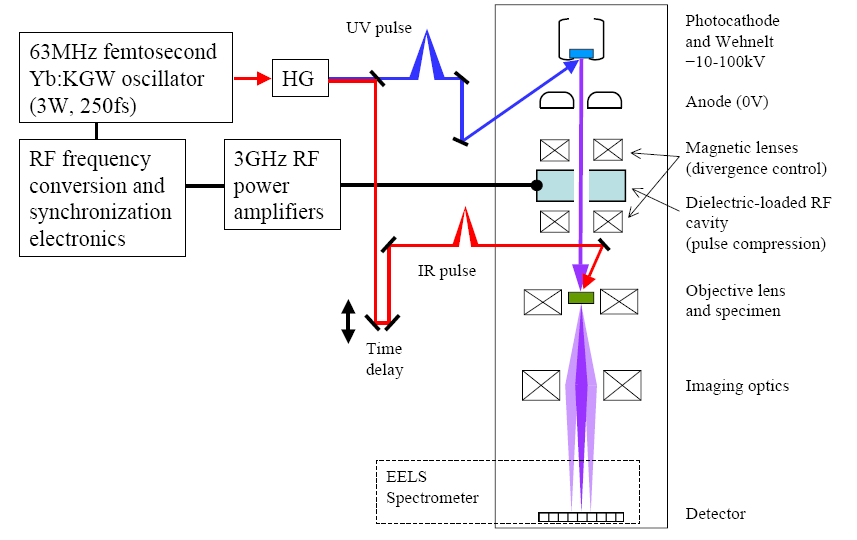
\includegraphics[width=0.85\linewidth]{UEM}};
      \node at (-3,-2) [text width=5cm] {
        \begin{itemize}
          \item<2-> Time-Integrated
          \item<3-> Stroboscopic
          \item<4-> Single-Shot
        \end{itemize}
      };
    \end{tikzpicture}
  \end{center}
\end{frame}

% added modes to above
%\begin{frame}{Operational Modes}
%  Along with the usual TEM modes of operation
%  \begin{itemize}
%    \item Imaging
%    \item Diffraction
%    \item HAADF
%    \item EELS
%    \item etc.
%  \end{itemize}
%  \uncover<2->{TR-EM offers an additional mode choice}
%  \begin{itemize}
%    \item<3-> Single-Shot (assumed mode for this talk)
%    \item<4-> Stroboscopic (requires repeatable process)
%    \item<5-> Time-integrated (Conventional operation)
%  \end{itemize}
%\end{frame}

\begin{frame}{Instruments in Development}
\begin{center}
\begin{tikzpicture}
  \node (image) {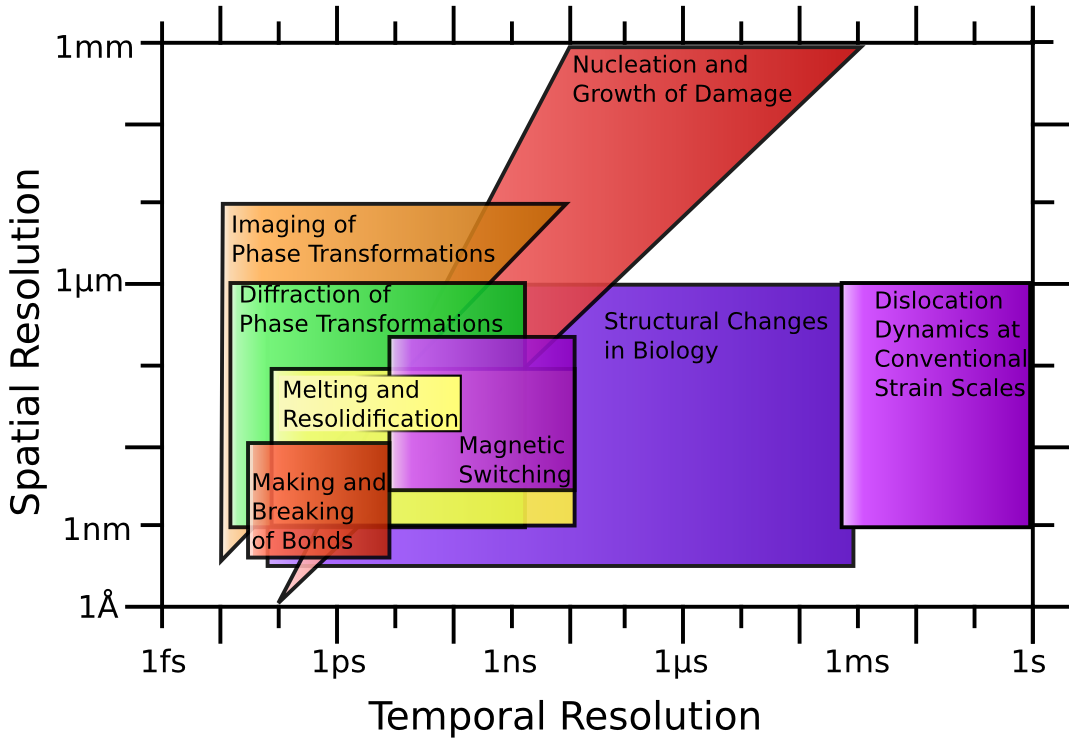
\includegraphics[width=0.7\linewidth]{Resolution}};
  \visible<2->{
    \node [
      star,
      star point ratio = 2,
      inner sep = 0.7mm,
      draw,
      fill=white,
      pin={[draw,fill=white,pin edge=thick] above:{\tiny TU-Berlin}}
    ] at (0.3,0.1) {};
    \node [
      star,
      star point ratio = 2,
      inner sep = 0.7mm,
      draw,
      fill=white,
      pin={[draw,fill=white,pin edge=thick] right:{\tiny UEM-2 Caltech}}
    ] at (0.3,-0.3) {};
    \node [
      star,
      star point ratio = 2,
      inner sep = 0.7mm,
      draw,
      fill=white,
      pin={[draw,fill=white,pin edge=thick,pin distance=0.6in] above:{\tiny Caltech stroboscopic}}
    ] at (-1.3,-0.3) {};
    \node [
      star,
      star point ratio = 2,
      inner sep = 0.7mm,
      draw,
      fill=white,
      pin={[draw,fill=white,pin edge=thick] right:{\tiny LLNL}}
    ] at (0.4,-0.6) {};
    \node [
      star,
      star point ratio = 2,
      inner sep = 0.7mm,
      draw,
      fill=white,
      pin={[draw,fill=white,pin edge=thick] right:{\tiny UC-Davis Bio-DTEM}}
    ] at (1.2,-1.1) {};
  }
  \end{tikzpicture}
  \end{center}
\end{frame}


\section{Physical Considerations}

\begin{frame}{Physical Considerations}
A major focus of my research has been to identify physical limitations, verify them, and propose and test solutions for them.\footcite{berger_dc_2009}
\begin{figure}
  \centering
  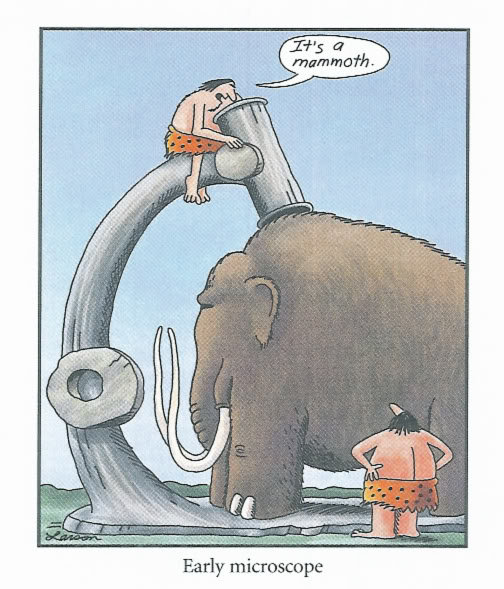
\includegraphics{mammoth}
\end{figure}
\end{frame}

\subsection{Difficulty Generating High Charge Ultrafast Pulses}
\begin{frame}{How Many Electrons are Needed?}
  The venerable \alert<2->{Rose Criterion}\footcite{Rose_1948} provides a guideline.
  \vfill
  \uncover<2->{
    \begin{block}{The Rose Criterion}
      For proper gray-scaling, 100 electrons are needed for each pixel in the detector.
    \end{block}
  }
  \vfill
  \begin{itemize}
    \item<3-> Imaging: Single-Shot (1k x 1k detector) $\rightarrow 10^8$ electrons
    \item<4-> Imaging: Stroboscopic same but over multiple shots
    \item<5-> Diffraction: (either mode) $\rightarrow \sim10^6$ electrons
  \end{itemize}
\end{frame}

\begin{frame}{Rose Criterion Demonstrated}
\begin{figure}
  \centering
  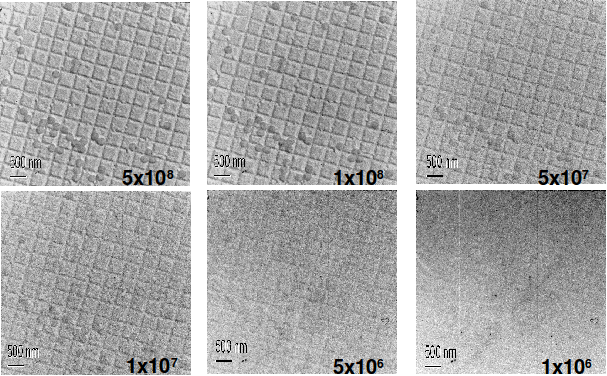
\includegraphics{ucdavis_resolution}
  \caption{From our collaborators at UCDavis / LLNL}
\end{figure}
\end{frame}

\begin{frame}{Short Pulse Child's Law}
  The Child-Langmuir Law describes the steady-state current limit in an electron gun. A similar law describes the limiting number of charges per pulse in a certain photoemission area.
  \begin{columns}
    \begin{column}{0.49\linewidth}
      \begin{tikzpicture}
        \filldraw
          [fill=black!50]
          (0,0) 
            node [name=photocathode1,below right]{}
          -- ++(1,0) node [above,midway] {-V}
          -- ++(0,-5)
            node [name=source,midway] {} 
          -- ++(-1,0)
          -- cycle
        ;
        \draw
          [dashed]
          (5,0) node (ground label) [above] {Ground}
          -- ++(0,-5)
        ;
        \node [left = 0.8cm of ground label,green] {$\vec{\text{E}}$};
        \only<1-2> {
          \foreach \x in {0,...,10}
            \draw [latex-,green] (1,-\x/2) -- ++(4,0);
        }
        \only<2> {
          \draw 
            [fill=blue!10]
            (2.0,-2.5)
            ellipse (0.3 and 2.5)
          ;
        }
        \only<3> {
          \foreach \x in {0,...,5}
            \draw [latex-,green] (1,-\x) -- ++(4,0);
          \foreach \x in {1,...,5}
            \draw [latex-,green] (2.3,0.5-\x) -- ++(2.7,0);
          \draw 
            [fill=blue!40]
            (2,-2.5)
            ellipse (0.3 and 2.5)
          ;
        }
        \only<4> {
          \foreach \x in {0,...,10}
            \draw [latex-,green] (2.3,-\x/2) -- ++(2.7,0);
          \draw 
            [fill=blue!80]
            (2,-2.5)
            ellipse (0.3 and 2.5)
          ;
        }
        \only <2-> {
          \node at (2,-2.5) {$\sigma$};
          \draw 
            [-latex,very thick] 
            (2.3,-2.25) 
            -- ++(0.5,0) 
              node [above] { $ \vec{v} $ }
          ;
        }
      \end{tikzpicture}
    \end{column}
    \begin{column}{0.49\linewidth}
      \begin{itemize}
        \item<2-> For low carrier density the electric field is unaffected
        \item<3-> For higher densities ($ \sigma / \epsilon_{0} \lesssim \text{E} $) the pulse begins to screen the photocathode
        \item<4-> For limiting densities ($ \sigma / \epsilon_{0} = \text{E} $) the pulse completely screens the photocathode stopping or distorting emission
      \end{itemize}
    \end{column}
  \end{columns}
\end{frame}

\begin{frame}{Implications of SPCL for TR-EM}
  The results of the previous concepts lead to a simple conclusion:
  \vfill
  \begin{block}{}
  \begin{figure}
    \centering
    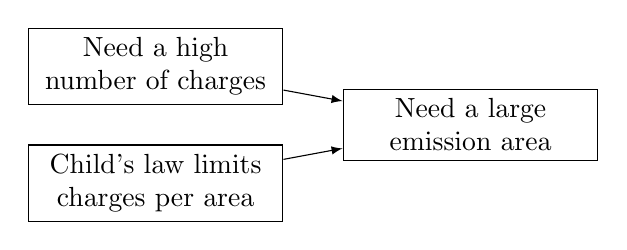
\begin{tikzpicture} [every node/.style={draw,fill=white,text badly centered,text width=3cm}]
      \node (charges)  {Need a high number of charges};
      \node (child) [below=0.5cm of charges] {Child's law limits charges per area};
      \node (result1) at ($(charges)!0.5!(child) + (4,0)$) {Need a large emission area};
      
      \draw [-latex] (charges) -- (result1);
      \draw [-latex] (child) -- (result1);
    \end{tikzpicture}
  \end{figure}
  \end{block}
  \vfill
  \uncover<2->{Further, large beam width necessitates custom, large bore TEM hardware}
\end{frame}

\begin{frame}{UEM vs. DTEM}
Definitions: \hfill (where TOF in photogun, $t_{gun} = \sqrt{ \frac{2 m d}{q E_{DC} } } \approx$ 0.1--1ns)
\vfill
  \begin{columns}
    \begin{column}{0.49\linewidth}
      \begin{block}{Ultrafast EM (UEM)}
      \centering
      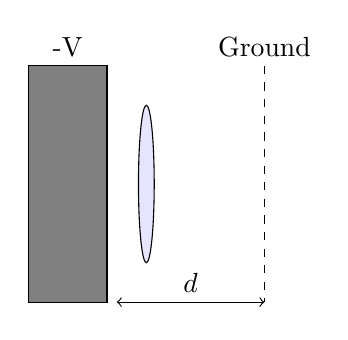
\begin{tikzpicture}
        \filldraw
          [fill=black!50]
          (0,0) 
            node [name=photocathode1,below right]{}
          -- ++(1,0) node [above,midway] {-V}
          -- ++(0,-3)
            node [name=source,midway] {} 
            node [name=bottom,pos=1] {}
          -- ++(-1,0)
          -- cycle
        ;
        \draw
          [dashed]
          (3,0) node (ground label) [above] {Ground}
          -- ++(0,-3)
        ;
        \draw 
          [fill=blue!10]
          (1.5,-1.5)
          ellipse (0.1 and 1)
        ;
        \draw [<->]
          (bottom)
          -- (bottom -| ground label)
            node [pos=0.5,above] {$d$}
        ;
      \end{tikzpicture}\\
      Short-pulse Child's Law applies\\
      $\tau_{pulse} < t_{gun}$
      \end{block}
    \end{column}
    \begin{column}{0.49\linewidth}
      \begin{block}{Dynamic TEM (DTEM)}
      \centering
      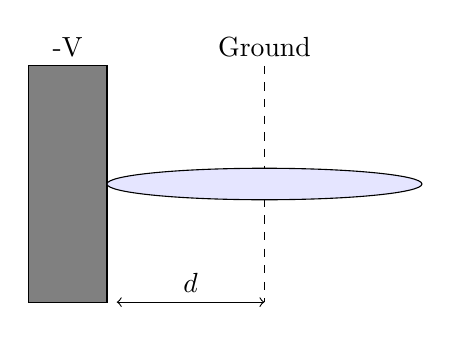
\begin{tikzpicture}
        \filldraw
          [fill=black!50]
          (0,0) 
            node [name=photocathode1,below right]{}
          -- ++(1,0) node [above,midway] {-V}
          -- ++(0,-3)
            node [name=source,midway] {}
            node [name=bottom,pos=1] {}
          -- ++(-1,0)
          -- cycle
        ;
        \draw
          [dashed]
          (3,0) node (ground label) [above] {Ground}
          -- ++(0,-3)
        ;
        \draw 
          [fill=blue!10]
          (3,-1.5)
          ellipse (2 and 0.2)
        ;
        \draw [<->]
          (bottom)
          -- (bottom -| ground label)
            node [pos=0.5,above] {$d$}
        ;
      \end{tikzpicture}\\
      Child-Langmuir Law applies\\
      $\tau_{pulse} > t_{gun}$
      \end{block}
    \end{column}
  \end{columns}
\end{frame}

\begin{frame}{UEM vs. DTEM}
\begin{center}
\begin{tikzpicture}
  \node (image) {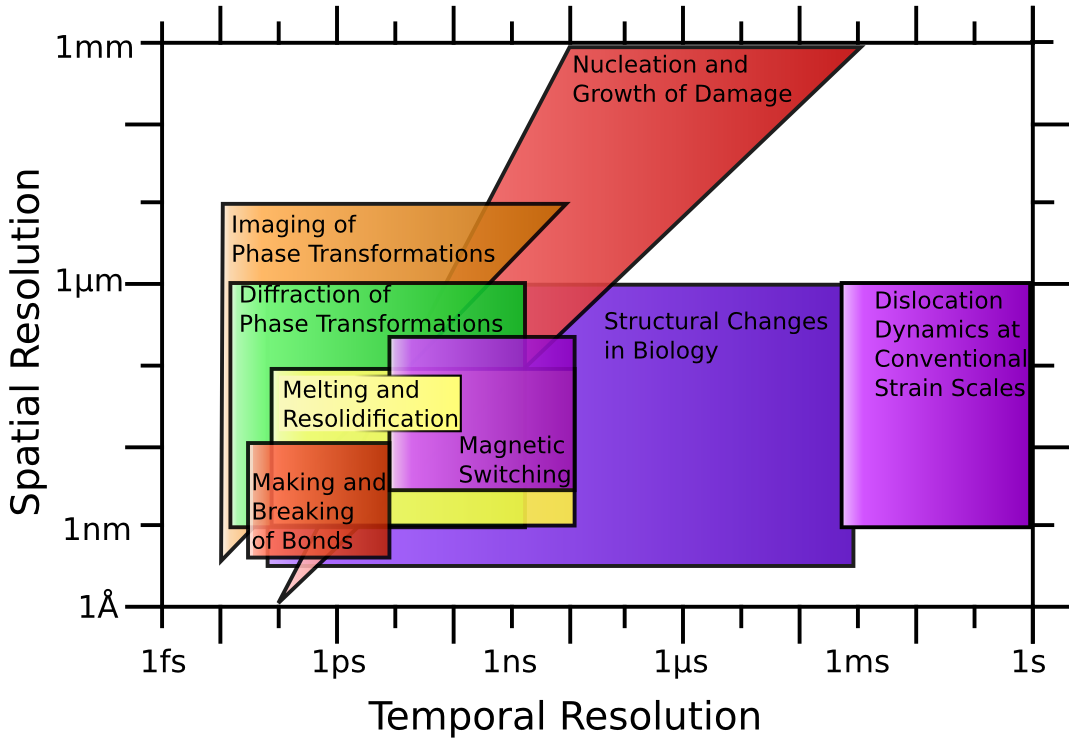
\includegraphics[width=0.7\linewidth]{Resolution}};
  \visible<2->{
    \node [
      star,
      star point ratio = 2,
      inner sep = 0.7mm,
      draw,
      fill=white,
      pin={[draw,fill=white,pin edge=thick] above:{\tiny TU-Berlin}}
    ] at (0.3,0.1) {};
    \node [
      star,
      star point ratio = 2,
      inner sep = 0.7mm,
      draw,
      fill=white,
      pin={[draw,fill=white,pin edge=thick] right:{\tiny UEM-2 Caltech}}
    ] at (0.3,-0.3) {};
    \node [
      star,
      star point ratio = 2,
      inner sep = 0.7mm,
      draw,
      fill=white,
      pin={[draw,fill=white,pin edge=thick,pin distance=0.6in] above:{\tiny Caltech stroboscopic}}
    ] at (-1.3,-0.3) {};
    \node [
      star,
      star point ratio = 2,
      inner sep = 0.7mm,
      draw,
      fill=white,
      pin={[draw,fill=white,pin edge=thick] right:{\tiny LLNL}}
    ] at (0.4,-0.6) {};
    \node [
      star,
      star point ratio = 2,
      inner sep = 0.7mm,
      draw,
      fill=white,
      pin={[draw,fill=white,pin edge=thick] right:{\tiny UC-Davis Bio-DTEM}}
    ] at (1.2,-1.1) {};
  }
  \visible<3->{
    \node[above=0.5mm of image] (text) {TOF in photogun, $t_{gun} = \sqrt{ \frac{2 m d}{q E_{DC} } } \approx$ 0.1--1ns};
  }
  \visible<4->{
    \draw<3->[fill=red!20,opacity=0.9] (-0.64,-1.85) rectangle (-0.17,2.56) node[left=0.1] (box) {};
    \draw<3->[->,thick,red] 
      (text.350) 
        to [out=-110,in=70] (box)
    %-- (box)
    ;
  }
  \visible<5->{
    \node [red] at (-2,2) {UEM};
    \node [red] at (3,2) {DTEM};
  }
\end{tikzpicture}
\end{center}
\end{frame}



\subsection{Need for Low Emittance Pulses}
\begin{frame}{Conservation of Emittance}
\begin{columns}
  \begin{column}{0.42\linewidth}
  \begin{center}
  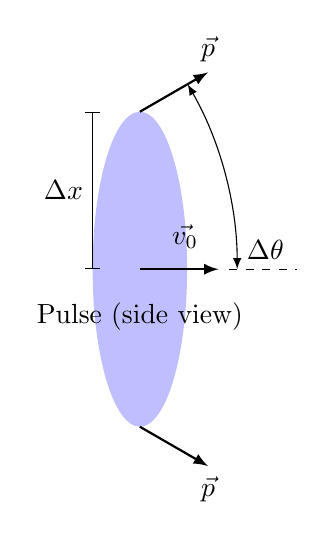
\begin{tikzpicture}
    \coordinate (spotsize) at (0,2);
    \coordinate (pulselength) at (0.6,0);
    \coordinate (pulse) at (0,0);
    \fill [blue!50, opacity=0.5]
      let
        \p1=(spotsize),
        \p2=(pulselength)
      in
      (pulse)
      ellipse (\x2 and \y1)
    ;
    \node [below=0.3 of pulse] {Pulse (side view)};
    \draw [|-|]
      let 
        \p1 = (spotsize)
      in
      ($(pulse) - (pulselength)$)
      -- node [left, pos=0.5] {$\Delta x$} ++(0,\y1)
    ;
    \draw[-latex, thick]
      (spotsize)
      -- 
        node [pos=0.7] (divangle) {} 
        node [pos=1,above] {$\vec{p}$}
        ++(30:1)
    ;
    \draw[-latex, thick]
      ($(pulse) - (spotsize)$)
      -- node [pos=1,below] {$\vec{p}$} ++(-30:1)
    ;
    \draw[thick, -latex]
      (pulse)
      -- ++(1,0) node [pos=1,label={above left:{$\vec{v_0}$}}] (end v) {}
    ;
    \draw[dashed]
      (end v)
      -- ++(1,0)
    ;
    \draw[latex-latex]
      let
        \p1 = (divangle)
      in
      (divangle)
      arc [
        start angle = 30,
        end angle = 0,
        radius = (\y1 / sin(30))
      ] 
      node [above right] {$\Delta \theta$} 
    ;
  \end{tikzpicture}
  \end{center}
  \end{column}
  \begin{column}{0.56\linewidth}
    \begin{block}<2->{Transverse Normalized Emittance}
      \begin{equation*}
        \varepsilon_{n,x} = \frac{1}{m c} \Delta x \Delta p_{x} 
          = \frac{v_0}{c} \Delta x \Delta \theta
      \end{equation*}
    \end{block}
    \begin{block}<3->{Liouville's Theorem}
      Emittance is conserved under aberration-free propagation
    \end{block}
    \begin{block}<4->{Emittance Growth}	
      Emittance may increase due to aberrations or other adverse conditions
    \end{block}
  \end{column}
\end{columns}
\end{frame}

\begin{frame}{To Improve Resolution}
%For a beam imaged fully on the detector:
  \begin{center}
  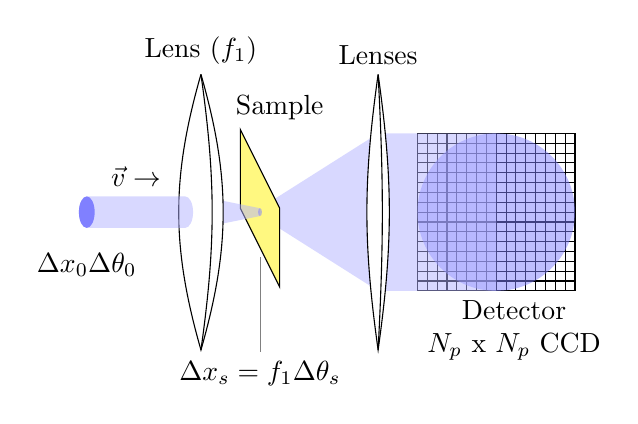
\begin{tikzpicture}[scale=0.5]
    \draw (-2,-2) node [below right,align=center] {Detector\\$N_p$ x $N_p$ CCD} rectangle (2,2);
    \draw [step=0.25] (-2,-2) grid (2,2);
    \fill[blue!50, opacity=0.5] (0,0) circle (2);
    \coordinate (lens1) at (-3,0);
    \coordinate (fplane) at (-6,0);
    \coordinate (lens2) at (-7.5,0);

    % beam from sample to detector
    \fill[blue!30, opacity=0.5]
      (0,2) 
      -- ($(lens1) + (0,2)$) 
      -- ($(fplane) + (0,0.1)$)
      -- ($(fplane) - (0,0.1)$)
      -- ($(lens1) - (0,2)$)
      -- (0,-2)
      --cycle;

    % sample
    \draw [fill=yellow!50]
      ($(fplane) + (-0.5,2.1)$)
      -- ++(0,-2)
      -- ++(1,-2)
        node [pos=0.5, pin={[pin distance=1.2cm]below:$\Delta x_s = f_1 \Delta \theta_s$}] {}
      -- ++(0,2)
        node [above=1cm] {Sample} 
      -- cycle
    ;

    % beam from objective to sample
    \fill[blue!30, opacity=0.5]
      ($(lens2) + (0,0.4)$)
      -- ($(fplane) + (0,0.1)$)
      -- ($(fplane) - (0,0.1)$)
      -- ($(lens2) - (0,0.4)$)
      -- cycle
    ;

    % beam spot on sample
    \fill[blue!50, opacity=0.5]
      (fplane) 
      ellipse (0.05 and 0.1)
    ;

    \draw [fill=white] 
      ($(lens1) + (0,3.5)$)
      node [above] {Lenses}
      to [out=262, in=98] ++(0,-7) 
      to [out=82, in=278] ++(0,7)
    ;
    \draw 
      ($(lens1) + (0,3.5)$)
      to [out=273, in=87] ++(0,-7) 
    ;
    \draw [fill=white] 
      ($(lens2) + (0,3.5)$)
      node [above] {Lens ($f_1$)}
      to [out=254, in=106] ++(0,-7)  
      to [out=74, in=286] ++(0,7)
    ;
    \draw 
      ($(lens2) + (0,3.5)$)
      to [out=278, in=82] ++(0,-7) 
    ;
    \fill[blue!30, opacity=0.5]
      ($(lens2) + (-0.4,0.4)$)
      -- ++(-2.5,0)
      node [black,opacity=1,above,pos=0.5] {$\vec{v} \rightarrow$}
      arc [
        start angle=90,
        end angle=270,
        x radius=0.2,
        y radius=0.4
      ]
      -- ++(2.5,0)
      arc [
        start angle=-90,
        end angle=90,
        x radius=0.2,
        y radius=0.4
      ]
    ;
    \fill[blue!50]
      ($(lens2) + (-2.9,0)$) 
      ellipse (0.2 and 0.4)
        node[below=0.4cm,black] {$\Delta x_0 \Delta \theta_0$}
    ;
  \end{tikzpicture}
  %\begin{block}{Resolution}
  %  Resolution = Spot size on sample / 1D Number of Pixels ($N_p$)
  %\end{block}
  %\uncover<2->{Example: 1$\mu$m spot and 1k x 1k CCD $\Rightarrow$ 1nm resolution}
  \end{center}
  \visible<2->{Resolution (per pixel):}
  \begin{equation*}
    \visible<2->{ \Delta X }
    \only<2>{ = \frac{\Delta x_s}{N_p} }
    \only<3->{ = \frac{\sqrt{\Delta x_s^2}}{N_p} }
    \visible<4->{ = \frac{\sqrt{\Delta x_s \Delta \theta_s f_1}}{N_p} }
    \visible<5->{ \ge \frac{\sqrt{\Delta x_0 \Delta \theta_0 f_1}}{N_p} }
  \end{equation*}
\end{frame}

\begin{frame}{Implication of Liouville's Theorem}
  Again results of the previous slides lead to a simple conclusion:
  \vfill
  \begin{block}{}
  \begin{figure}
    \centering
    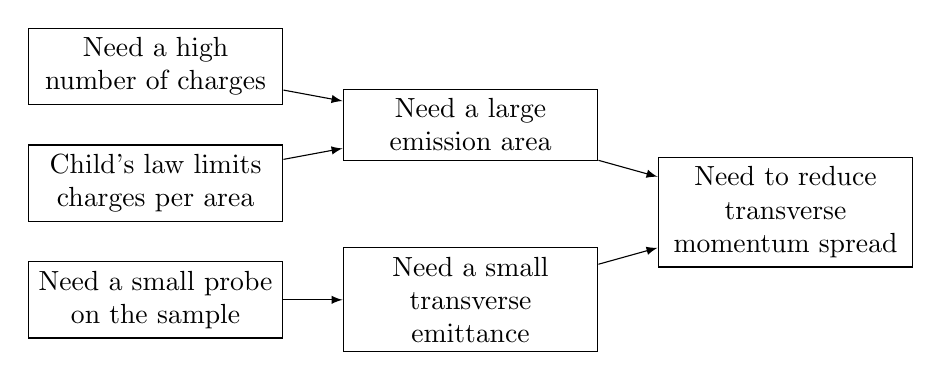
\begin{tikzpicture} [every node/.style={draw,fill=white,text badly centered,text width=3cm}]
      \node (charges)  {Need a high number of charges};
      \node (child) [below=0.5cm of charges] {Child's law limits charges per area};
      \node (probe) [below=0.5cm of child] {Need a small probe on the sample};
      \node (result1) at ($(charges)!0.5!(child) + (4,0)$) {Need a large emission area};
      \node (emittance) at ($(probe) + (4,0)$) {Need a small transverse emittance};
      \node (result2) at ($(result1)!0.5!(emittance) + (4,0)$) {Need to reduce transverse momentum spread};
      
      \draw [-latex] (charges) -- (result1);
      \draw [-latex] (child) -- (result1);
%      \draw [-latex] (result1.south) to [out=270,in=135] (emittance.north west);
      \draw [-latex] (result1) -- (result2);
      \draw [-latex] (probe) -- (emittance);
      \draw [-latex] (emittance) -- (result2);
    \end{tikzpicture}
  \end{figure}
  \end{block}
  \vfill
\end{frame}

\begin{frame}{Reducing the Transverse Momentum}
  \begin{columns}
    \begin{column}{0.54\linewidth}
    Methods for reducing transverse momentum
    \begin{itemize}
      \item Aperture the beam at a Fourier plane
      \begin{itemize}
        \item<5-> Loss of electrons
        \item<6-> Dynamic lensing at aperture
      \end{itemize}
      \item<7-> Reduce transverse momentum upon emission
    \end{itemize}
    \end{column}
    \begin{column}{0.44\linewidth}
      \begin{center}
      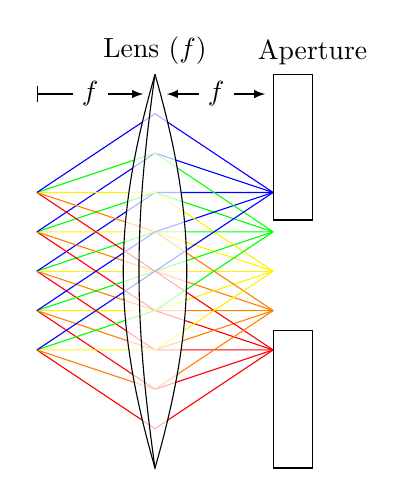
\begin{tikzpicture}[scale=0.5]
        \node (origin) at (0,0) {};
        \foreach \y/\slide in {0/2,1/3,-1/3,2/4,-2/4} {
          \foreach \x/\color in {-2/red, -1/orange, 0/yellow, 1/green, 2/blue} {
            \draw<\slide->[color=\color]
              (0,\y)
              -- ++(3,\x)
              -- (6,\x)
            ;
          }
        }
        \filldraw[fill=white, opacity=0.7, draw=black, draw opacity=1] 
          (3,5)
          node [above,opacity=1] {Lens ($f$)}
          to [out=254, in=106] ++(0,-10)  
          to [out=74, in=286] ++(0,10)
        ;
        \draw 
         (3,5)
          to [out=262, in=98] ++(0,-10) 
        ;
        \draw
          (7,5) node [above] {Aperture}
          rectangle (6,1.3)
        ;
        \draw
          (7,-5)
          rectangle (6,-1.5)
        ;
        \draw [|-latex]
          (0,4.5)
          -- ++(2.7,0)
          node [pos=0.5,fill=white] {$f$}
        ;
        \draw [latex-latex]
          (3.3,4.5)
          -- ++(2.5,0)
          node [pos=0.5,fill=white] {$f$}
        ;
      \end{tikzpicture}
      Transverse momentum reduction by aperturing
      \end{center}
    \end{column}
  \end{columns}
\end{frame}


\section{Photocathode Engineering/Reducing $\Delta p_{\smallT}$}
\begin{frame}{Simple Photoemission from a Metal}
  \begin{center}
  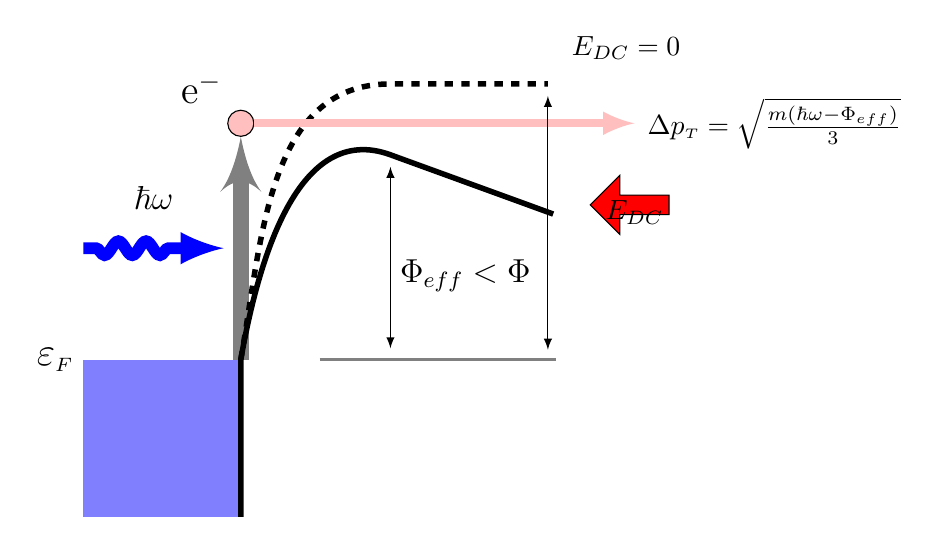
\begin{tikzpicture}[every node/.style={transform shape}]
    \node (electron) [circle,fill=pink,draw,label=above left:{\Large e$^{-}$}] {};
    \fill [blue!50] 
      ($(electron) + (-2cm,-3cm)$) node [left,black] {\Large $\varepsilon_{\scriptscriptstyle F} $}
      -- ++(+2cm,0) node (surface) {}
      -- ++(0,-2cm) node (sub-surface) {}
      -- ++(-2cm,0);
    
    \draw [gray,line width=2mm,->,>=latex']
      (surface.center) 
      -- (electron) node [midway] (photon) {};
    
    \draw [line width=1.5mm,<-,>=latex,decorate,blue,decoration={snake,pre=lineto,pre length=7mm}]
      (photon)
      -- ++(-2cm,0) node [midway,above=3mm,black] {\large $ \hbar \omega $};
      
    \draw [gray,line width=0.5mm] 
      (surface) ++(1cm,0) -- ++(3cm,0) node [pos=0.3] (x-phi) {};
  
    \draw [line width=0.7mm,dashed]
      (surface.center) to [out=80,in=180] ($(electron -| x-phi) + (0,5mm)$) -- ++(2cm,0) node [label=above right:{$ E_{DC}=0 $}] (upper-no-field) {};
    \draw [line width=0.7mm]
      (sub-surface.center) -- (surface.center) to [out=80,in=160] ($(electron -| x-phi) - (0,4mm)$) node (upper) {} -- ++(-20:2.2cm);
  
    \draw [line width=1mm,->,>=latex,pink] 
      (electron) -- ++(5cm,0) 
        node (exit) {}
        node [right,black] {$\Delta p_{\smallT} = \sqrt{\frac{m (\hbar \omega - \Phi_{eff})}{3}}$};
    \node [below=of exit,shape=single arrow,minimum height=1cm,draw,fill=red,label={[yshift=-5mm]below:{$ E_{DC} $}},rotate=180] {};
    
    \draw [<->,>=latex] (x-phi) -- (upper) node [pos=0.4,right] {\large $ \Phi_{eff} < \Phi $};
    \draw [<->,>=latex] (upper-no-field) -- (upper-no-field |- surface.north);
  \end{tikzpicture}
  \end{center}
\end{frame}

\begin{frame}{Driving a Plasmon (Back-Illuminated)}
  \begin{columns}
  \begin{column}{0.54\linewidth}
    \begin{center}
    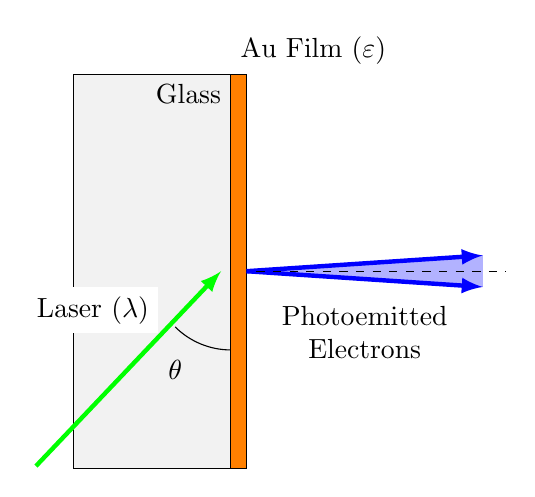
\begin{tikzpicture}
      \filldraw [fill=gray!10]
      (0,0)
      node [below left] {Glass}
      rectangle (-2,-5)
      ;
      \filldraw
        [fill=orange]
        (0,0) 
        node [name=photocathode1,above right]{Au Film ($\varepsilon$)}
        -- ++(0.2,0)
        -- ++(0,-5)
        node [name=source,midway] {} 
        -- ++(-0.2,0)
        -- (0,0)
        node [name=laser,midway] {}
        -- cycle
      ;
      \draw
        [-latex,ultra thick,green] 
        ($(laser) + (-135:3.5)$) 
        -- (laser.west)
        node [left=0.3,name=laser label,pos=0.8,black,fill=white] {Laser ($\lambda$)}
      ;
      \fill
        [blue!30]
        (source.center)
        -- ++(3,2mm)
        -- ++(0,-4mm)
        -- cycle
      ;
      \draw
        [-latex,ultra thick,blue]
        (source.center)
        -- ++(3,2mm)
      ;
      \draw
        [-latex,ultra thick,blue]
        (source.center)
        -- ++(3,-2mm)
        node [name=electron label,pos=0.5,black,below=0.2,align=center]{Photoemitted\\Electrons}
      ;
      \draw
        [dashed]
        (source)
        -- ++(3.3,0)
      ;
      \draw 
        ($(laser) + (0,-1)$) 
        arc (-90:-135:1)
        node [below=0.3] {$\theta$}
      ;
    \end{tikzpicture}
    \end{center}
  \end{column}
  \begin{column}{0.44\linewidth}
    \begin{figure}
      \centering
      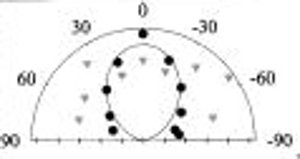
\includegraphics[scale=0.8]{plasmon_reduction_angle}
      \caption{The measured angular distribution of photoelectrons
in the plane of incidence (dots) and perpendicular to that (triangles), as
well as a fit to a $\cos^2\theta$ distribution.\footcite{zawadzka_evanescent}}
    \end{figure}
  \end{column}
  \end{columns}
\end{frame}

\begin{frame}{Driving a Plasmon (Front-Illuminated)}
  \begin{columns}
    \begin{column}{0.49\linewidth}
  \begin{center}
  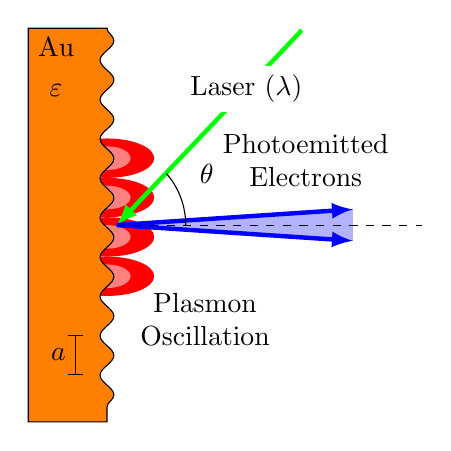
\begin{tikzpicture}
    \filldraw
      [fill=orange]
      (0,0) 
      node [name=photocathode1,below right]{Au}
      node [below=1mm of photocathode1] {$\varepsilon$}
      -- ++(1,0)
      decorate [decoration=snake,segment length=5mm]{ 
        -- ++(0,-5)
        node [name=source,midway] {} 
      } 
      -- ++(-1,0)
      -- cycle
    ;
    \draw [|-|]
      ($(source) + (-4mm,-14mm)$)
      -- ++(0,-5mm)
      node [midway,left] {$a$}
    ;
    \begin{pgfonlayer}{background}
      \foreach \x in {8.5mm,3.5mm,-1.5mm,-6.5mm} {
        \fill<2->
          [fill=red]
          ($(source) + (0,\x)$) 
          ellipse (6mm and 2.5mm)
        ;
        \fill<2->
          [fill=red!50]
          ($(source) + (0,\x)$)
          ellipse (3mm and 1.5mm)
        ;
      }
    \end{pgfonlayer}
    \draw
      [-latex,ultra thick,green] 
      ($(source) + (45:3.5)$) 
      -- (source.east)
      node [name=laser label,pos=0.3,black,fill=white] {Laser ($\lambda$)}
    ;
    \fill<3->
      [blue!30]
      (source.east)
      -- ++(3,2mm)
      -- ++(0,-4mm)
      -- cycle
    ;
    \draw<3->
      [-latex,ultra thick,blue]
      (source.east)
      -- ++(3,2mm)
    ;
    \draw<3->
      [-latex,ultra thick,blue]
      (source.east)
      -- ++(3,-2mm)
      node [name=electron label,pos=0.8,black,above=0.5,align=center]{Photoemitted\\Electrons}
    ;
    \draw
      [dashed]
      (source)
      -- ++(4,0)
    ;
    \draw 
      ($(source) + (1,0)$) 
      arc (0:41:1)
      node [right=0.3] {$\theta$}
    ;
    \node<2-> [anchor=west,align=center] at ($(source) + (0.3,-1.2)$) {Plasmon\\Oscillation};
  \end{tikzpicture}
  \end{center}
    \end{column}
    \begin{column}{0.49\linewidth}
      To drive a surface plasmon by front-illumination align so that:
      \begin{align*}
        k_{SP} =& k_{laser}^{\parallel} + k_{G}\\
        \sin(\theta) =& \sqrt{ \frac{\varepsilon}{1+\varepsilon} } - \frac{\lambda}{a}
      \end{align*}
      where $\varepsilon$ is the metal's dielectric constant
      \begin{block}<4->{Why Gold?}
        Surface plasmon frequency is near 2nd harmonic (green) of our Yb:KGW laser
      \end{block}
    \end{column}
  \end{columns}
\end{frame}

\begin{frame}{First Attempt (Gold on Glass)}
  \begin{columns}
    \begin{column}{0.49\linewidth}
      First attempt:
      \begin{itemize}
        \item Commercial optical grating
        \item Gold on glass substrate
        \item 750 lines per mm
      \end{itemize}
      \visible<2->{
        \begin{block}{Result}
          Insufficient heat conduction though glass substrate
        \end{block}
      }
    \end{column}
    \begin{column}{0.49\linewidth}
      \begin{figure}
        \centering
        \visible<3->{
          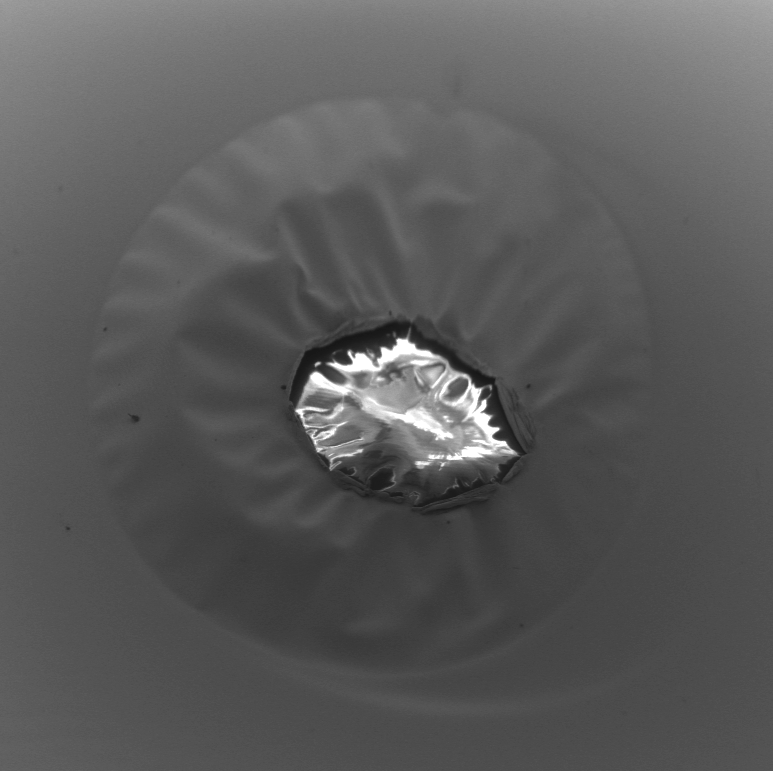
\includegraphics[width=0.8\linewidth]{Damage}
        }
      \end{figure}
    \end{column}
  \end{columns}
\end{frame}

\begin{frame}{Second attempt (Gold on FIB milled silicon)}
  To avoid heat problems:
  \begin{itemize}
    \item Silicon substrate
    \begin{itemize}
      \item<2-> Focused Ion Beam (FIB) milled at Argonne Nat'l Lab (ANL)
      \item<3-> Near sinusoidal shape
      \item<3-> $\sim 1 \mu$m periodicity
      \item<4-> Several ($\sim10$) 100$\mu$m x 100$\mu$m patches
      \item<4-> Several hours of milling
    \end{itemize}
    \item<5-> Gold coated at UIC Nano Core Facility (NCF)
    \begin{itemize}
      \item<6-> 300 nm thickness
      \item<6-> Chromium binding layer
    \end{itemize}
  \end{itemize}
  
\end{frame}

\begin{frame}{Sinusoidal Nanopatterned Photocathode}
  \begin{tikzpicture}
    \begin{pgfonlayer}{below-main}
      \node[name=low,label=below:Low Mag]{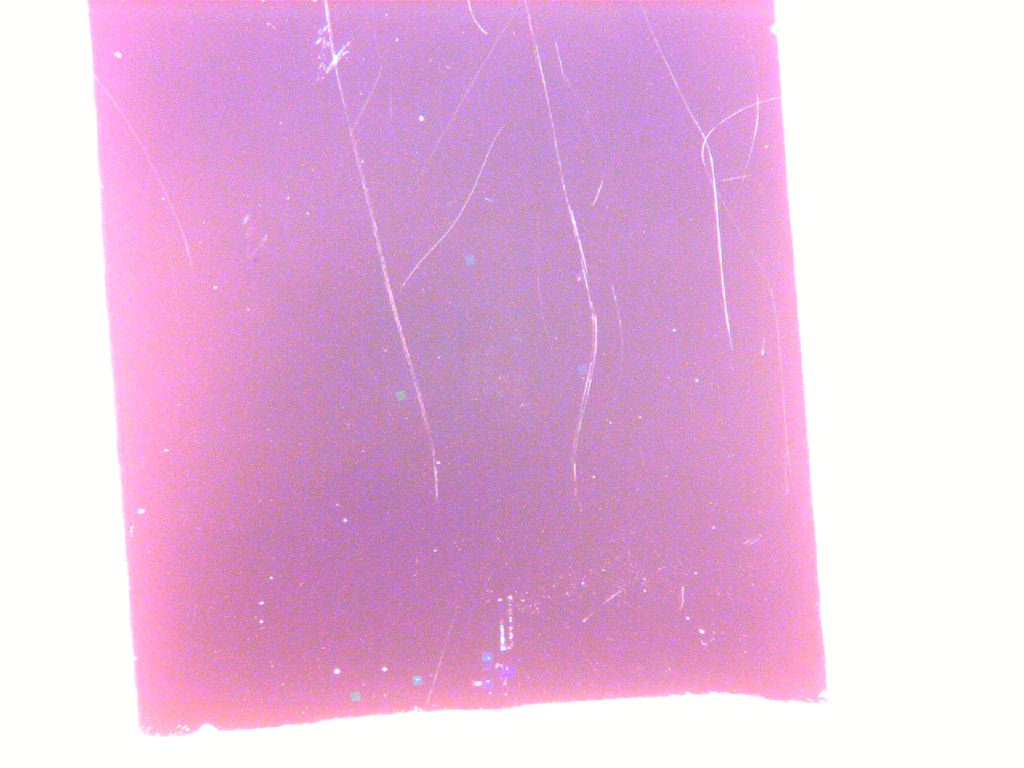
\includegraphics[width=2in]{FIB-low}};
    \end{pgfonlayer}
    \draw<2->
      (-7mm,8mm) node [name=low-top-left] {}
      -- ++(12mm,0) node [name=low-top-right] {}
      -- ++(0,-10mm) node [name= low-bottom-right] {}
      -- ++(-12mm,0) node [name= low-bottom-left] {}
      -- cycle
    ;
    \visible<3->{
      \node [
        inner sep=0,
        right=8mm of low.center,
        yshift=2.3cm,
        name=medium,
        label=above:Medium Mag
      ] {
        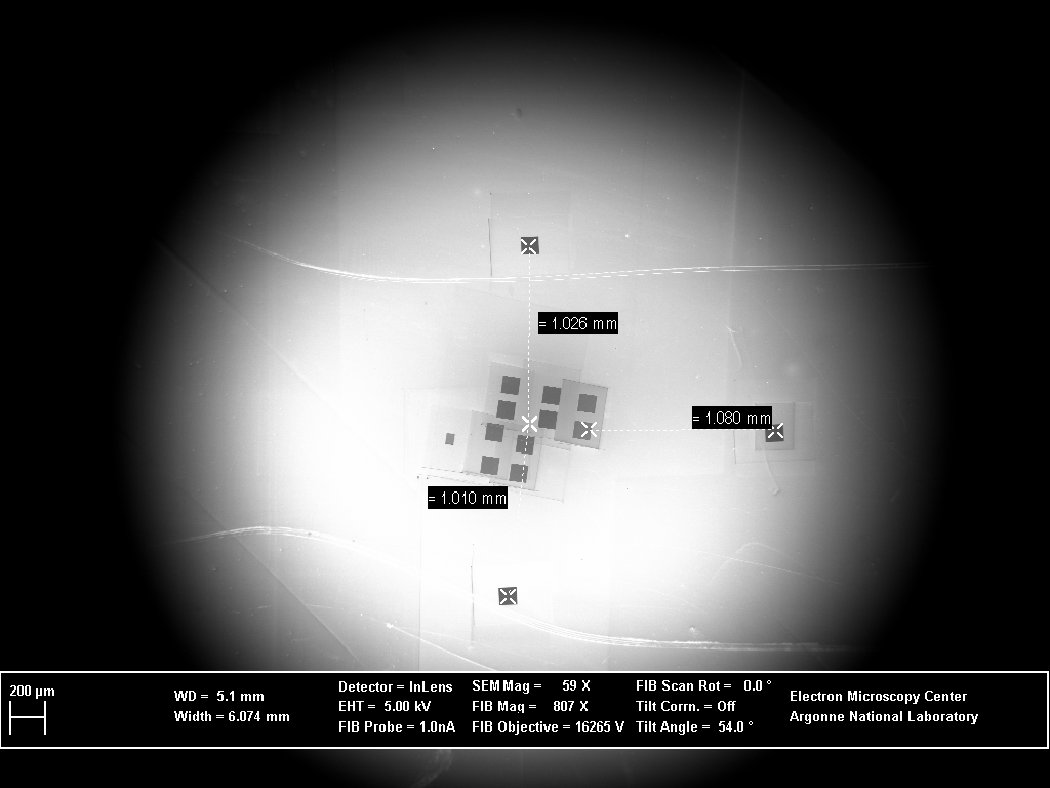
\includegraphics[width=2in]{FIB-medium}
      }
      ;
    }
    \begin{pgfonlayer}{below-main}
      \draw<3-> (low-top-left.center) -- (medium.north west);
      \draw<3-> (low-top-right.center) -- (medium.north east);
      \draw<3-> (low-bottom-left.center) -- (medium.south west);
      \draw<3-> (low-bottom-right.center) -- (medium.south east);
    \end{pgfonlayer}
    \begin{pgfonlayer}{above-main}
      \visible<5->{
        \node [
          inner sep=0,
          name=high,
          below right=1cm of medium.center,
          label=below:High Mag
        ] {
          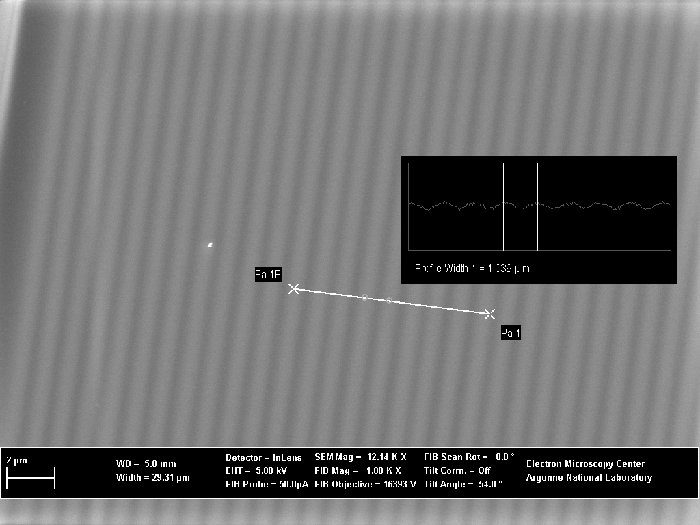
\includegraphics[width=2in]{FIB-high}
        };
      }
    \end{pgfonlayer}
    \node [name=feature, right=2.3mm of medium.center,inner sep=0.7mm,yshift=-0.5mm] {};
    \draw<4->
      (feature.north east)
      -- (feature.north west)
      -- (feature.south west)
      -- (feature.south east)
      -- cycle
    ;
    \draw<5-> (feature.north east) -- (high.north east);
    \draw<5-> (feature.north west) -- (high.north west);
    \draw<5-> (feature.south east) -- (high.south east);
    \draw<5-> (feature.south west) -- (high.south west);
  \end{tikzpicture}
\end{frame}

\begin{frame}{Sinusoidal Nanopatterned Photocathode --- Results}
  \begin{center}
    \begin{tikzpicture}
      \node {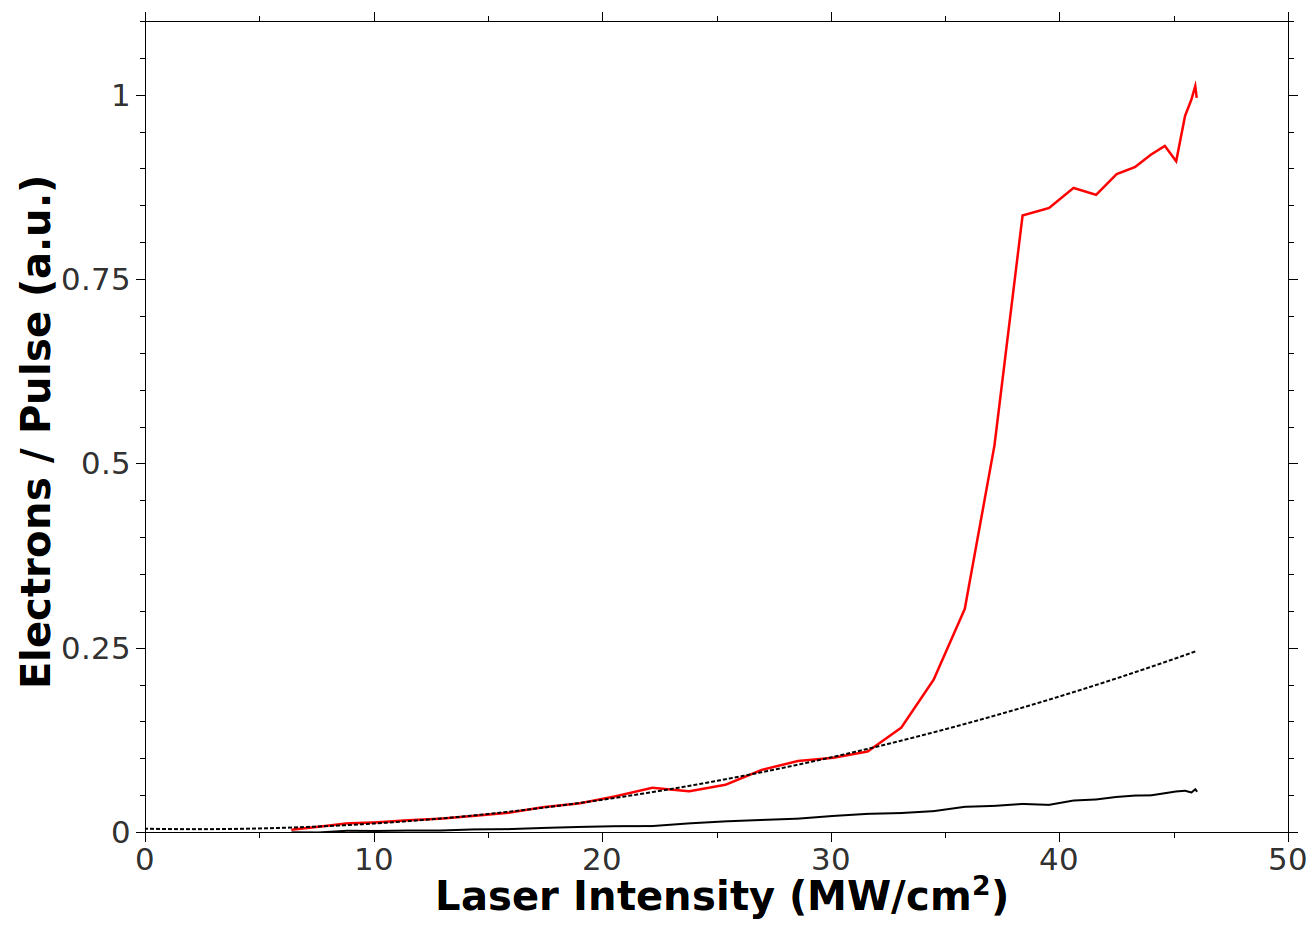
\includegraphics{Graph1}};
      \node<2> at (-1.8,1.8) [draw] {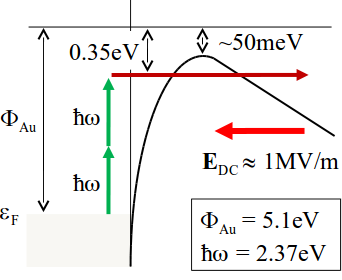
\includegraphics[width=1.2in]{PE_diag_0}};
      \node<3> at (-1.8,1.8) [draw] {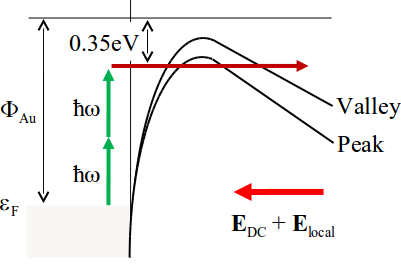
\includegraphics[width=1.2in]{PE_diag_1}};
      \node<4> at (-1.8,1.8) [draw] {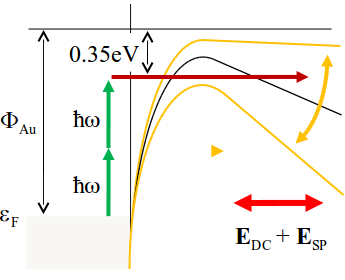
\includegraphics[width=1.2in]{PE_diag_2}};
      
      \node<1,3-4> at (2.1,2.8) [red,align=right] {Plasmon Enhanced\\Photoemission};
      \node<1> at (3.5,-0.7) {Fit $I^2$};
      
      \node<1-2> at (-1,-1.5) (TwoPhoton Label) [align=left] {Two Photon\\Photoemission};
      \draw<1-2> [thick,-latex]
        (TwoPhoton Label)
        to [out=0,in=110] (2.7,-2.2)
      ;
      
      \node<2> 
        at (3,1.7) 
        [label={below:Isotropic $\Delta p_{\scriptscriptstyle T}$}] 
        {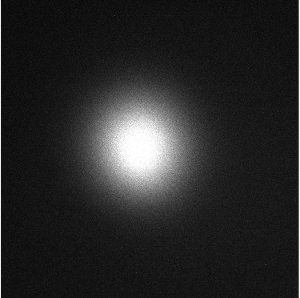
\includegraphics[width=1in]{final-fourier-2photon-036}}
      ;
      
      \node<3> 
        (fourier image)
        at (-2,-1) 
        [
          shape=rectangle callout, callout relative pointer={(0.9,-0.5)}, 
          draw, fill=white
        ] 
        {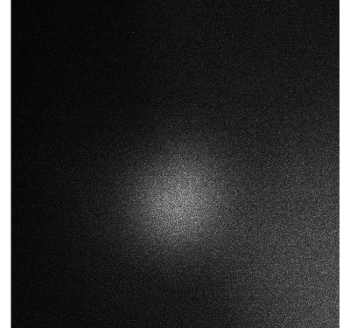
\includegraphics[width=1in]{final-fourier-022}}
      ;
      \node<3> [right=0.2 of fourier image] {Isotropic $\Delta p_{\scriptscriptstyle T}$};
      
      \node<4>
        at (-1.5,-1)
        [
          shape=rectangle callout, callout relative pointer={(1,-0.2)}, 
          draw, fill=white, align=left
        ] 
        {Onset of barrier suppression\\$\Rightarrow E_{SP} \approx$ 40MV/m}
      ;
      
      \node<5-> 
        at (-1.8,-1.4)
        [
          shape=rectangle callout, callout relative pointer={(1.9,-0.45)}, 
          draw, fill=white, align=left
        ] 
        {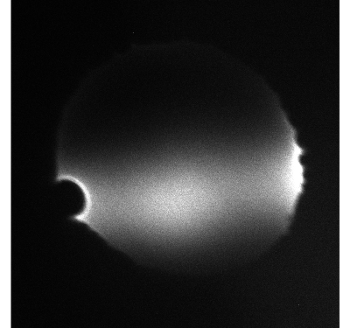
\includegraphics[width=0.7in]{final-fourier-026}}
      ;
      \node<5-> 
        at (0.5,0)
        [
          shape=rectangle callout, callout relative pointer={(0.7,-0.4)}, 
          draw, fill=white, align=left
        ] 
        {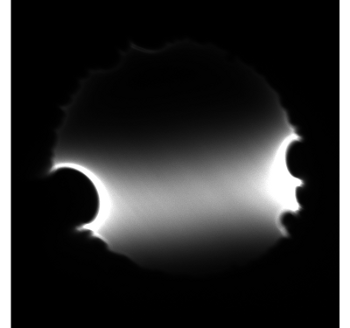
\includegraphics[width=0.7in]{final-fourier-030}}
      ;
      \node<5-> 
        at (1.2,2.2)
        [
          shape=rectangle callout, callout relative pointer={(1,0)}, 
          draw, fill=white, align=left
        ] 
        {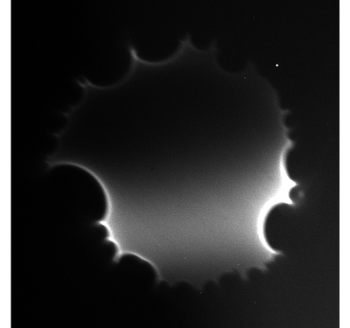
\includegraphics[width=0.7in]{final-fourier-038}}
      ;
      \node<5->
        at (-2,1.8)
        {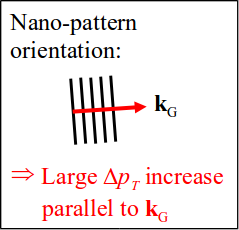
\includegraphics[width=1in]{PE_diag_3}}
      ;
    \end{tikzpicture}
  \end{center}
\end{frame}

\begin{frame}{Understanding Observed $\Delta p_{\scriptscriptstyle T}$ Increase}
  Is the 1D broadening due to the plasmon or the surface?
  \begin{center}
    \begin{tikzpicture}
  \draw [thick,->,green] 
    (0,0) -- ++(3,0) 
      node [pos=0.5,below,black,align=center] {$k_L \sin \theta$\\$\theta \approx 39^{\circ}$}
  ;
  \draw [thick,->,red]
    (3,0) -- ++(2,0)
      node [pos=0.5,below,black] {$k_G$}
  ;
  \draw [thick,->,blue]
    (0,0.2) -- ++(5,0)
      node [pos=0.5,black,above] {$k_{SP}$}
  ;
  \node at (7,0) {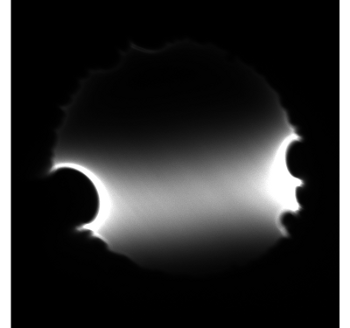
\includegraphics{final-fourier-030.png}};
  \draw [very thick,red] (6,-0.4) -- ++(9:2.2);

  \draw [thick,->,green] 
    (0,-3.5) -- ++(3,0) 
      node [pos=0.5,below,black,align=center] {$k_L \sin \theta$\\$\theta \approx 47^{\circ}$}
  ;
  \draw [thick,dashed,green] 
    (3,-3.5) -- (4,-3.5)
      node [above,black,pos=0.8] {$45^{\circ}$}
  ;
  \draw [thick,->,red]
    (3,-3.5) -- ++(1.4,1.4)
      node [pos=0.4,left,black] {$k_G$}
      coordinate [pos=1] (end)
  ;
  \draw [thick,->,blue]
    (0,-3.5) -- (end)
      node [pos=0.5,black,above] {$k_{SP}$}
  ;
  \node at (7,-3) {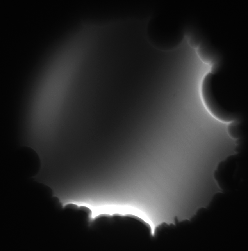
\includegraphics{rotated.png}};
  \draw [very thick,green,dashed] 
    (6,-2.7) -- ++(9:2.2)
      node [pos=0.7,below, white] {$45^{\circ}$}
      coordinate [pos=1] (rotate end)
  ;
  \draw [very thick,red]
    (rotate end) -- ++(234:2.2)
  ;
\end{tikzpicture}

  \end{center}
\end{frame}

\begin{frame}{Trenched Photocathode}
  \begin{columns}
    \begin{column}{0.54\linewidth}
      Grooved Photocathode
      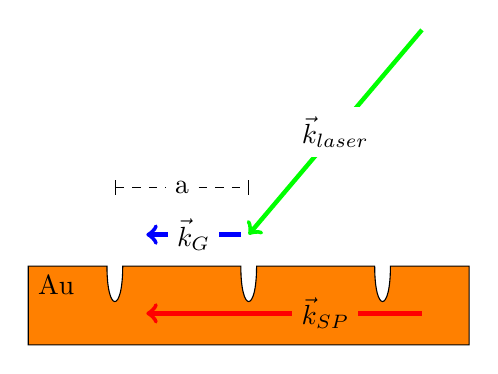
\begin{tikzpicture}
        \draw 
          [fill=orange]
          (0,0)
            node [below right] {Au}
          -- (1,0)
            .. controls (1,-0.6) and (1.2,-0.6)
          .. (1.2,0)
          -- (2.7,0)
            .. controls (2.7,-0.6) and (2.9,-0.6)
          .. (2.9,0)
          -- (4.4,0)
            .. controls (4.4,-0.6) and (4.6,-0.6)
          .. (4.6,0)
          -- (5.6,0)
          -- (5.6,-1)
          -- (0,-1)
          -- cycle
        ;  
        \draw [|-|,dashed]
          (1.1,1)
          -- (2.8,1)
            node [pos=0.5,fill=white] {a}
        ;
    
        \draw [ultra thick,red,->]
          (5,-0.6)
          -- (1.5,-0.6)
            node [pos=0.35,black,fill=orange] {$\vec{k}_{SP}$}
        ;
        \draw [ultra thick,green,->]
          (5,3)
          -- (2.8,0.4)
            node [pos=0.5,black,fill=white] {$\vec{k}_{laser}$}
        ;
        \draw [ultra thick, blue, ->]
          (2.7,0.4)
          -- (1.5,0.4)
            node [pos=0.5,black,fill=white] {$\vec{k}_{G}$}
        ;
      \end{tikzpicture}
    \end{column}
    \begin{column}{0.44\linewidth}
      \begin{align*}
        k_{SP} =& k_{laser}^{\parallel} + m \cdot k_{G}\\
        \sin(\theta) =& \sqrt{ \frac{\varepsilon}{1+\varepsilon} } - \frac{ m \lambda }{a}
      \end{align*}
      \begin{block}{}
        \begin{itemize}
          \item<2-> Retains periodic structure
          \item<3-> Reduced $\nabla_{\perp} E_{SP}$
          \item<4-> Additional Fourier components
          \item<5-> Easier to FIB mill
        \end{itemize}
      \end{block}
      \visible<6->{\alert{Update: Couldn't drive plasmon!}}
    \end{column}
  \end{columns}
\end{frame}

\begin{frame}
  \begin{columns}
    \begin{column}{0.45\linewidth}
      \begin{figure}
        \centering
        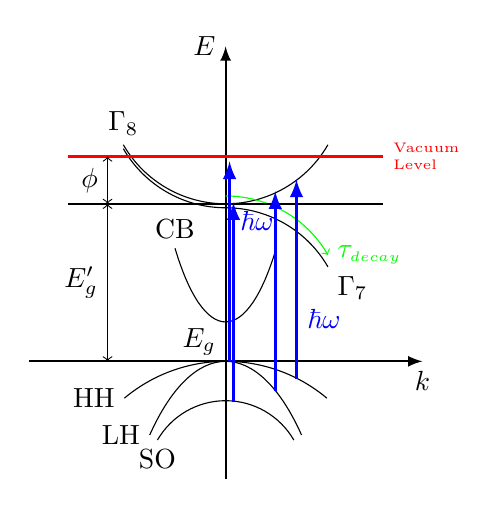
\begin{tikzpicture}
  % grid
  %\draw (-3,-2) grid (3,5);

  % axes
  \draw [-latex, thick] (-2.5,0) -- (2.5,0) node [below] {$k$};
  \draw [-latex, thick] (0,-1.5) -- (0,4) node [left] {$E$};

  % bands
  %\draw (-1,-0.5) .. controls (-0.25,0.25) .. (0,0);
  %\draw (-1,-1) .. controls (-0.5,0) and (0.5,0) .. (1,-1);
  \coordinate (so gamma) at (0,-0.5);
  \draw<3-> (so gamma) arc [start angle=90, end angle=30,  radius=1];
  \draw<3-> (so gamma) arc [start angle=90, end angle=150, radius=1]
    node [below] {SO};

  \coordinate (origin) at (0,0);
  \draw (origin) arc [start angle=90, end angle=50,  radius=2];
  \draw (origin) arc [start angle=90, end angle=130, radius=2]
    node [left] {HH};

  \draw (origin) arc [start angle=90, end angle=50,  x radius=1.5, y radius=4];
  \draw (origin) arc [start angle=90, end angle=130, x radius=1.5, y radius=4]
    node [left] {LH};

  \coordinate (cb gamma) at (0,0.5);
  \draw (cb gamma) arc [start angle=-90, end angle=-50,  x radius=1, y radius=4];
  \draw (cb gamma) arc [start angle=-90, end angle=-130, x radius=1, y radius=4]
    node [above] {CB};
  \node [left] at ($(cb gamma)!0.5!(origin)$) {$E_g$};

  \coordinate (gamma 8) at (0,2);
  \draw<2-> (gamma 8) arc [start angle=-90, end angle=-30,  radius=1.5];
  \draw<2-> (gamma 8) arc [start angle=-90, end angle=-150, radius=1.5]
    node [above] {$\Gamma_{8}$};

  \coordinate (gamma 7) at (0,1.95);
  \draw<7-> (gamma 7) arc [start angle=90,  end angle=30,   radius=1.5]
    node [below right] {$\Gamma_{7}$};
  \draw<7-> (gamma 7) arc [start angle=-90, end angle=-150, radius=1.5];
  \draw<7-> [green,->] (gamma 7) ++(0,0.15) arc [start angle=90,  end angle=30,   radius=1.5]
    node [right] {$\tau_{{\scriptscriptstyle decay}}$};

  % defined energies
  \coordinate (energies) at (-1.5,0);
  \draw<4-> [thick] ($(gamma 8) + (-2,0)$) -- ++(4,0);
  \draw<4-> [<->] (energies) -- (energies |- gamma 8)
    node [pos=0.5,left] {$E_{g}^{\prime}$};

  \coordinate (vacuum level) at ($(gamma 8) + (0,0.6)$);
  \draw [thick,red] ($(vacuum level) + (-2,0)$) -- ++(4,0)
    node [right,align=left,font=\tiny] {Vacuum\\Level};
  \draw<4-> [<->] (energies |- gamma 8) -- (energies |- vacuum level)
    node [pos=0.5,left] {$\phi$};

  % photon excitation
  \draw<1> [-latex, blue, very thick] (0.05,0) -- ++(0,2.54)
    node [right,pos=0.7] {$\hbar \omega$};
  \draw<3-> [-latex, blue, very thick] (0.1,-0.52) -- ++(0,2.54);
  \draw<2-> [-latex, blue, very thick] (0.63,-0.38) -- ++(0,2.54);
  \draw<2-> [-latex, blue, very thick] (0.9,-0.23) -- ++(0,2.54)
    node [right,pos=0.3] {$\hbar \omega$};

\end{tikzpicture}

      \end{figure}
    \end{column}
    \begin{column}{0.53\linewidth}
      \begin{tabular}{|c|c|c|}
        \hline
          & GaSb & InSb \\ \hline
        \rowvisible{4-}{$E_{g}^{\prime}$}{3.77eV}{3.59eV} \\ \hline
        \rowvisible{4-}{$\phi$}{0.99eV}{1.18eV} \\ \hline
        \rowvisible{5-}{Excess $E$}{$\sim$0.35eV}{$\sim$0.41eV} \\
        \rowvisible{5-}{$\Rightarrow$ initial $T_e$}{4200K}{4900K} \\ \hline
        \rowvisible{8-}{$m^{*}(\Gamma_8)$}{$0.3 m_0$}{$0.5 m_0$} \\ \hline
      \end{tabular}
      \vspace{3mm}
      \visible<6->{
        $\exp(-\phi / k_{{\scriptscriptstyle B}} T_e) \approx 0.6$
        \begin{itemize}
          \item thermionic photoemission!
        \end{itemize}
      }
      \visible<7->{
        Cooling rates of $\sim$1600 K/ps from
        \begin{itemize}
          \item LO phonons 
          \item fast decay via $\Gamma_7$
        \end{itemize}
      }
    \end{column}
  \end{columns}
\end{frame}


\section{Hardware Development}
\begin{frame}{RRC Laboratory}
  Intrumentation development at UIC's Research Resources Center --- East
  \begin{center}
    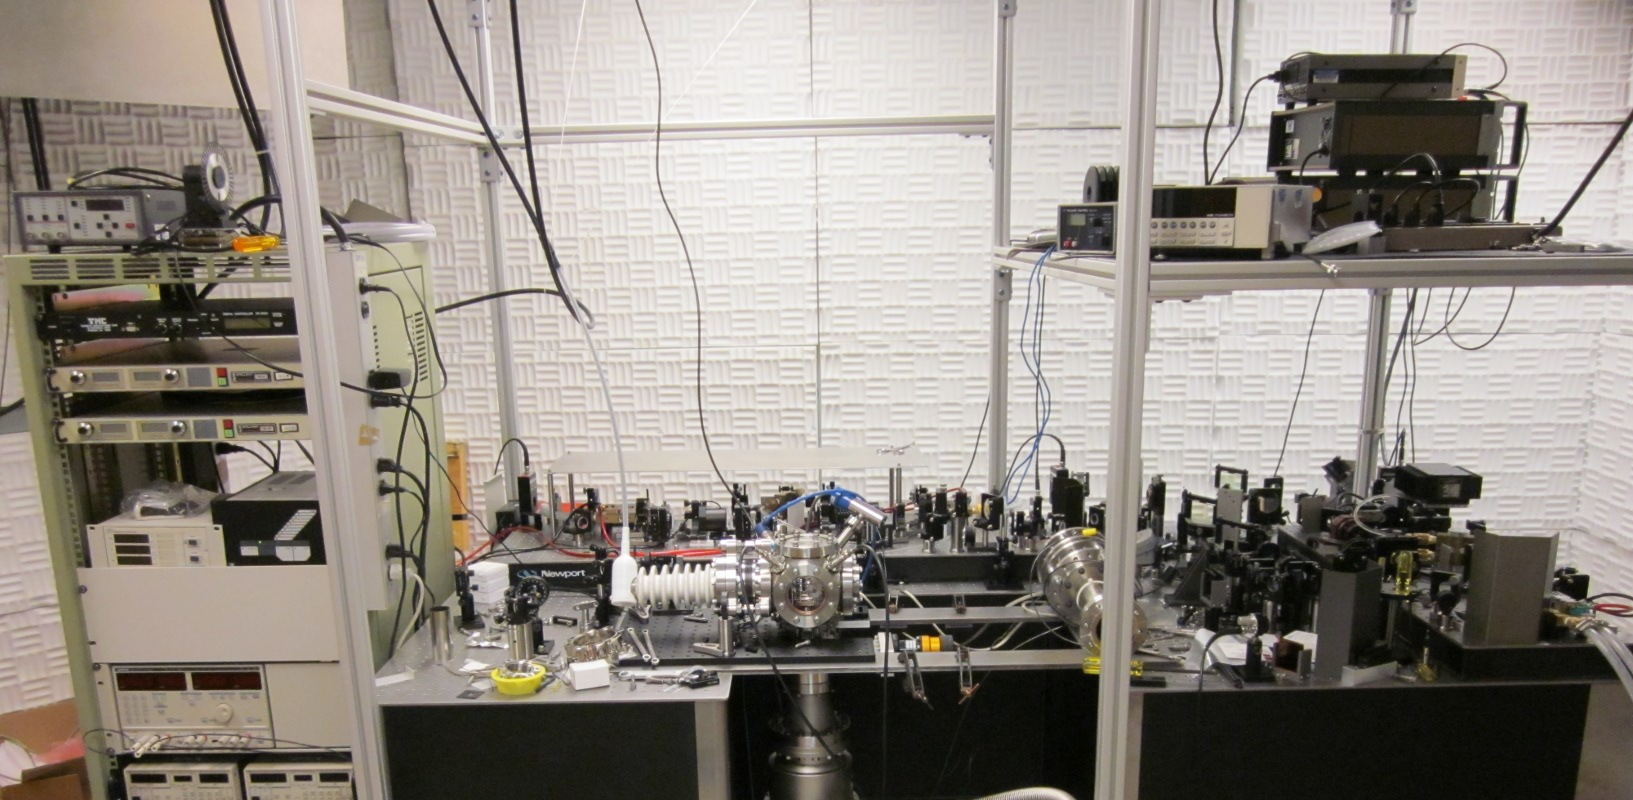
\includegraphics{lab}
  \end{center}
\end{frame}

\begin{frame}{Togawa Accelerator Design}
  The Togawa accelerator\footcite{togawa_ceb6_2007} provides
  \begin{columns}
    \begin{column}{0.49\linewidth}
      \begin{itemize}
        \item<2-> Large aperture
        \item<3-> Relatively flat electric field
        \item<4-> Low divergence near anode aperture
      \end{itemize}
      \begin{figure}
        \centering
        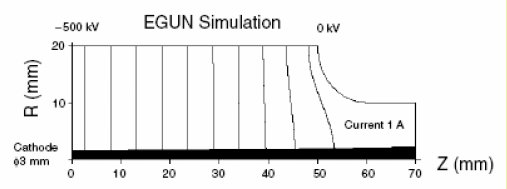
\includegraphics[width=0.9\linewidth]{Togawa_Plot}
      \end{figure}
    \end{column}
    \begin{column}{0.49\linewidth}
      \begin{itemize}
        \item<5-> Large laser angular acceptance
        \item<5-> Large photocathode area (Wehnelt)
        \item<5-> Smooth easily polished surfaces
      \end{itemize}
      \begin{figure}
        \centering
        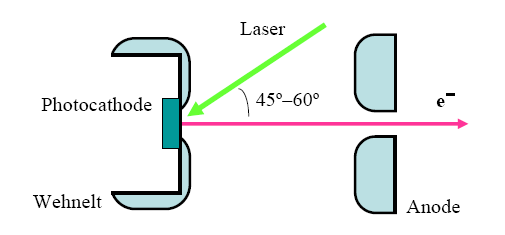
\includegraphics[width=0.9\linewidth]{Togawa}
      \end{figure}
    \end{column}
  \end{columns}
\end{frame}

\begin{frame}{Hardware Development}
  \begin{columns}
    \begin{column}{0.49\linewidth}
      Togawa Wehnelt / Anode
      \begin{figure}
        \centering
        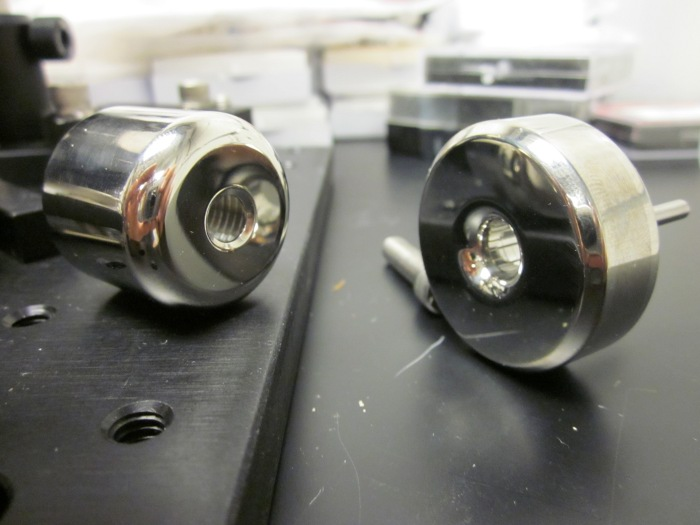
\includegraphics{anode_cathode}
      \end{figure}
    \end{column}
    \begin{column}{0.49\linewidth}
      Custom deflection plates
      \begin{figure}
        \centering
        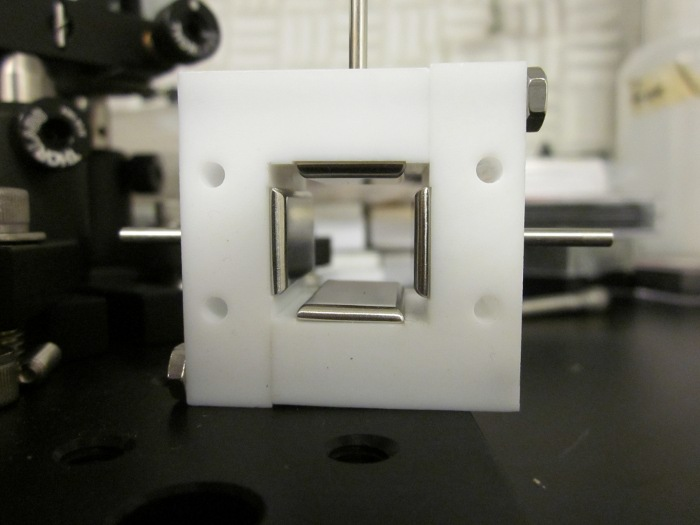
\includegraphics{deflector}
      \end{figure}
    \end{column}
  \end{columns}
  \begin{figure}
    \centering
    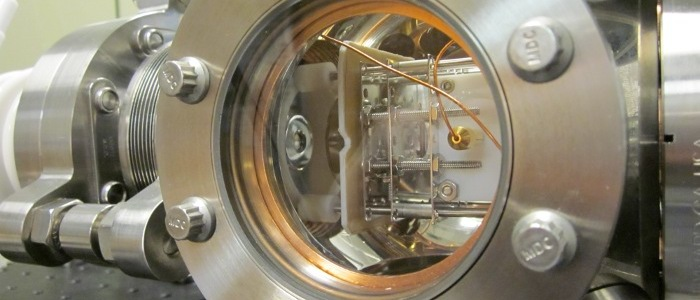
\includegraphics{chamber}
  \end{figure}
\end{frame}

\begin{frame}{Magnetic Lenses}
  For both imaging our photocathode emission and its momentum distribution (Fourier plane)
  \begin{itemize}
    \item<2-> Custom design\footcite{el-kareh_electron_1970}
    \item<3-> Large bore (aperture)
    \item<4-> High permeability pole piece (NiFe alloy $\mu \approx $50000)
  \end{itemize}
  \uncover<5->{As a pair, will be used to correct for RF cavity's inherent divergence}
\end{frame}

\begin{frame}{Magnetic Lenses Installed}
  \begin{figure}
    \centering
    \begin{tikzpicture}
      [every pin edge/.style={white,thick}]
      \begin{pgfonlayer}{background}
        \node {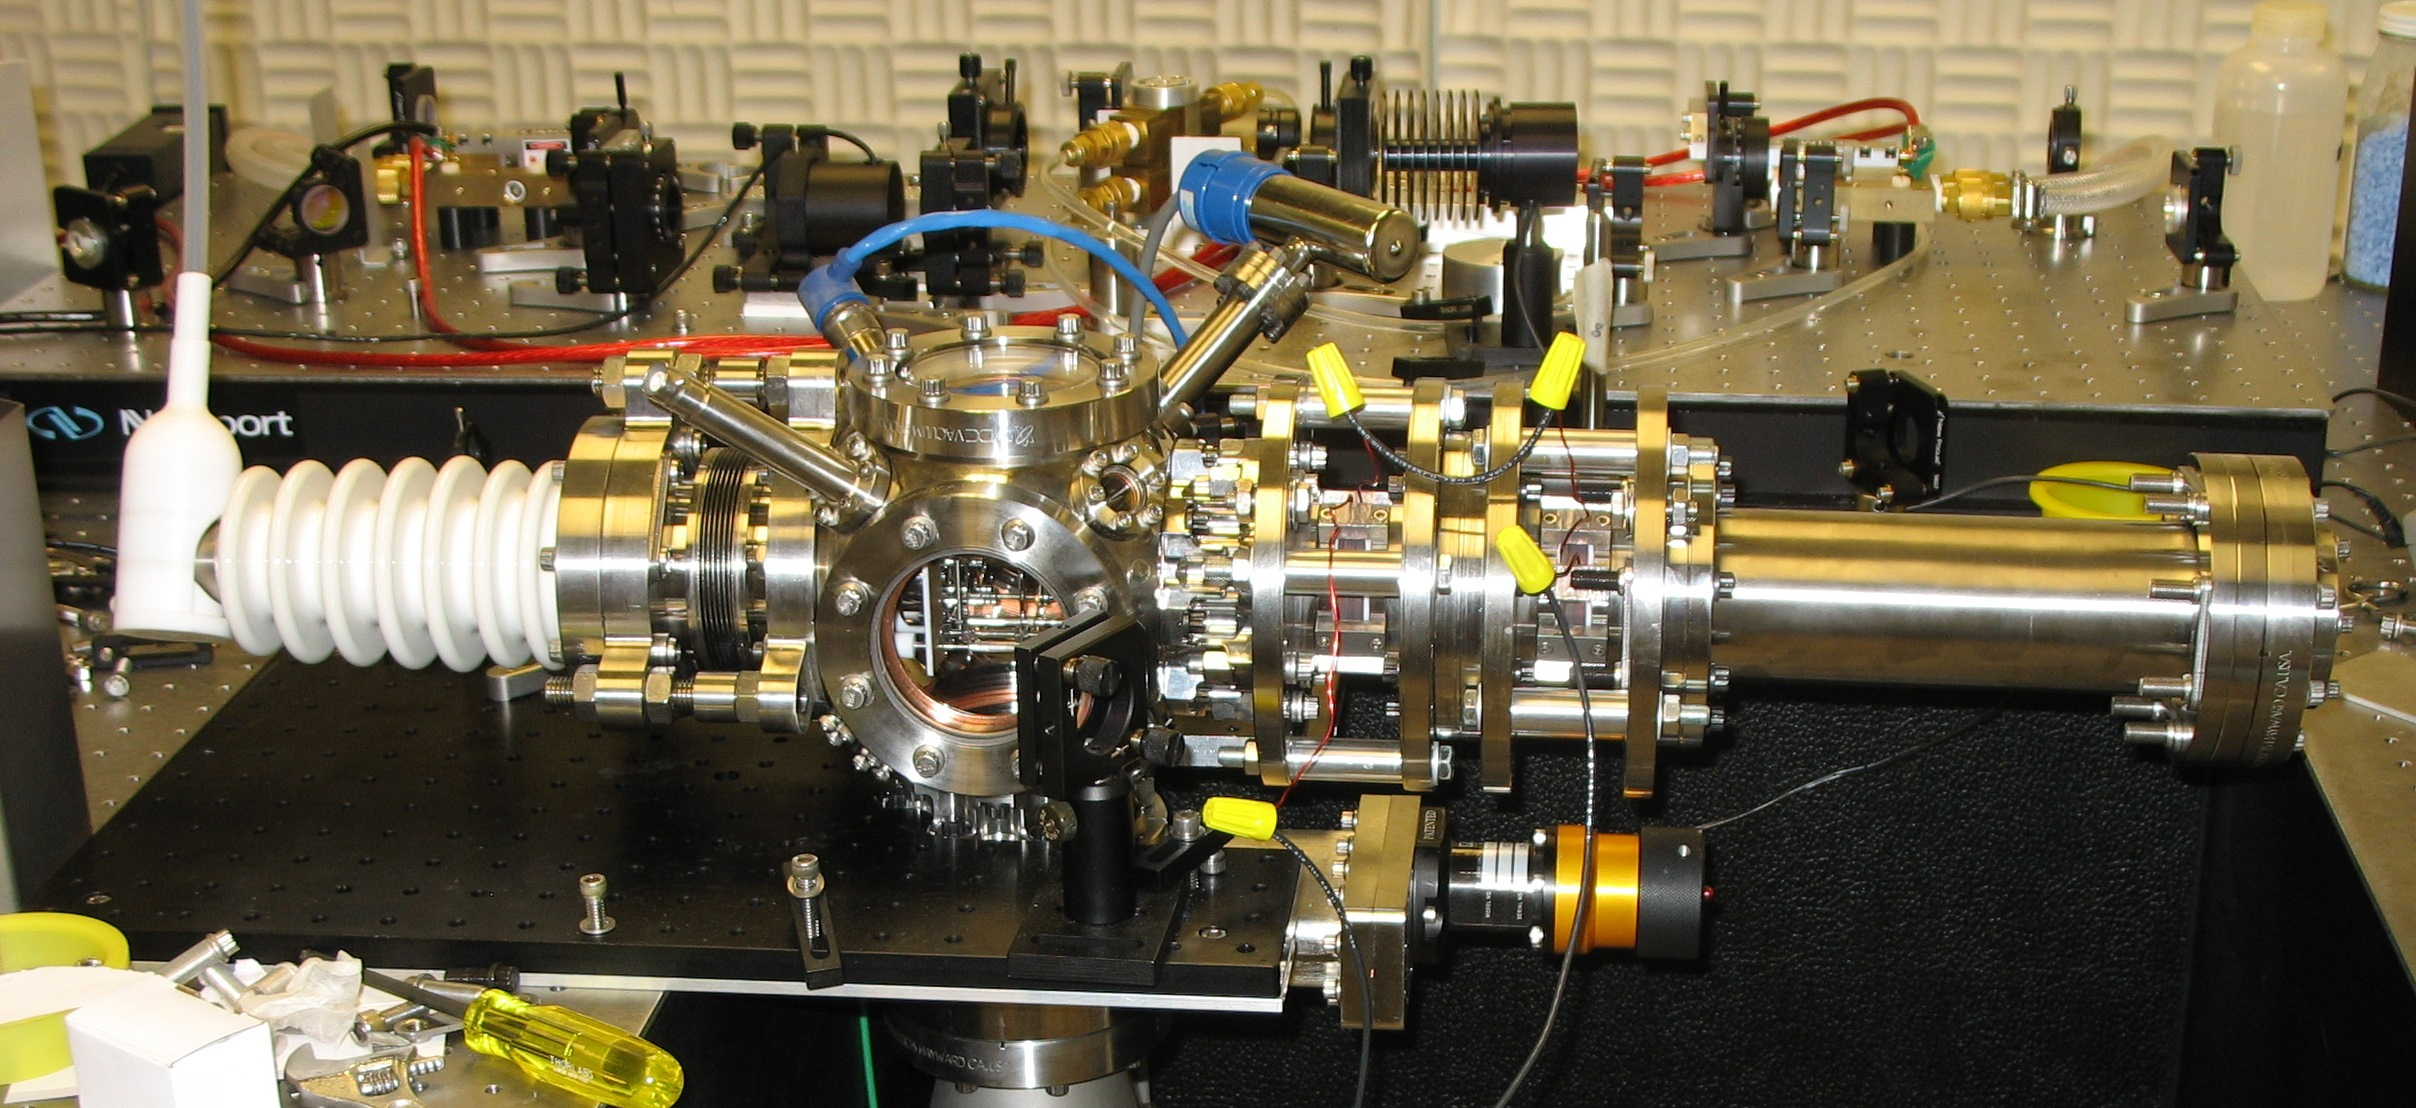
\includegraphics[width=0.9\linewidth]{column_lenses}};
      \end{pgfonlayer}
      \draw<2->
        [fill=orange] 
        (-2,-0.5)
        -- ++(0.2,0)
          node [midway,pin={below,fill=white:Photocathode}] {}
        -- ++(0,1)
          node [midway,inner sep=0.1] (source) {}
        -- ++(-0.2,0)
        -- cycle
      ;
      \draw<2->
        [fill=red]
        ($(source) + (2.35,0) $) node [inner sep=2mm] (lens1) {}
        arc (180:160:2)
        arc (20:-20:2)
          node (label lens1) {}
        arc (200:180:2)
      ;
      \draw<2->
        [fill=red]
        ($(source) + (3.4,0) $) node [inner sep=2mm] (lens2) {}
        arc (180:160:2)
        arc (20:-20:2)
          node (label lens2) {}
        arc (200:180:2)
      ;
      \node<2-> at ($(lens1)!0.5!(lens2) + (0,-1.5)$) (lens label) [red,fill=white] {Magnetic Lenses};
      \foreach \x in {1,2}
        \draw<2-> [white,thick] (lens label) -- (label lens\x);
      \draw<2-> 
        [fill=green!40]
        ($(source) + (6.5,0)$) node [inner sep=0] (detector) {}
          ellipse (0.2 and 0.5) 
            node at ($(source) + (6.5,-0.5)$) [pin={below,fill=white:Detector}] {}
      ;
      \draw<3->
        [green,very thick]
        (-5.2,-0.7)
        -- (-0.7,-0.7)
          node [pos=0.2,below=2mm,fill=white] {Laser}
        -- (source.east)
      ;
      \draw<5-> [fill=gray!60]
        ($(lens1)!0.5!(lens2) + (-0.05,0.5)$)
        node [pin={above,fill=white:{RF Cavity}}] {}
        rectangle ++(0.3,-1)
      ;
      \begin{pgfonlayer}{below-main}
        \fill<4->
          [blue!40]
          (source)
          -- (lens1.north)
          -- (lens2.north)
          -- (detector.east)
            node [midway,above=5mm,fill=white] {Electron Beam}
          -- (lens2.south)
          -- (lens1.south)
        ;
      \end{pgfonlayer}
    \end{tikzpicture}
  \end{figure}
  \visible<6->{And yes, we fixed the drooping column mount}
\end{frame}

\begin{frame}{Primary Laser Oscillator}
  Diode-pumped Thermal Lens Shaped (TLS) Yb:KGW primary laser:
  \begin{itemize}
    \item<2-> 250 fs pulse duration
    \item<3-> 2W output at 63MHz (31 nJ)
    \item<4-> Fundamental: 1047nm ($\hbar \omega$ = 1.2eV)
    \item<5-> 2$\hbar \omega = $ 2.47eV (524nm): $\Rightarrow$ Au plasmon, 2 photon over Ta
    \item<6-> 4$\hbar \omega = $ 4.75eV (262nm): $\Rightarrow$ 1 photon over Ta
    \item<7-> Adjustable laser cavity length allows matching:
    \begin{itemize}
      \item<7-> Laser repetition rate
      \item<7-> RF cavity resonance frequency
    \end{itemize}
  \end{itemize}
  \begin{figure}
    \centering
    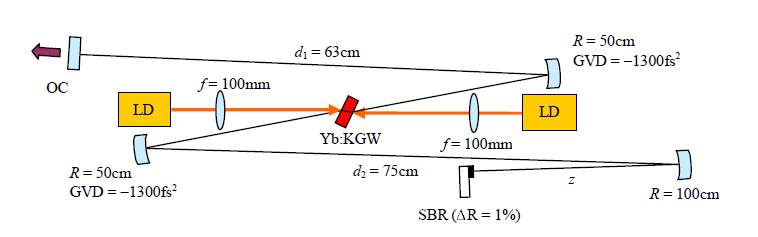
\includegraphics{laser_schematic}
  \end{figure}
\end{frame}



\section{Simulation}
\begin{frame}{Modeling Outline}
Propagating a very dense pulse will require extra planning. A model for designing a UEM column needs:
	\begin{itemize}[<+->]
	    \item Generation dynamics
		\item Propagation dynamics
		\item Acceleration and gun effects
		\item Lenses and/or compressors	
		\item Apertures (?)
		\item Speed (multiple runs for optimization)
	\end{itemize}
No model existed that had all these features.
\end{frame}

\begin{frame}{Pulse Modeling}
	Analytic Gaussian (AG) model of Michalik and Sipe\footcite{michalik_analytic_2006}: 
	\begin{itemize}
		\item<2-> Self-similar Gaussian electron packet
		\item<3-> 6D (3 position \& 3 momentum) moment analysis
		\item<4-> Mulitdimensional Gaussian integral
		\item<5->[$\Rightarrow$] Reduces free-space propagation dynamics to six first order coupled differential equations!
	\end{itemize}
    While this model is the propagation engine of my model, alone it lacks:
    \begin{itemize}
      \item<6-> Electron-optical elements
      \item<7-> Realistic initial conditions
    \end{itemize}
\end{frame}

\begin{frame}{AG Model Extension\footcite{berger_semi-analytic_2010}}
\begin{columns}
  \begin{column}{0.54\linewidth}
    The extended AG model adds:
    \begin{itemize}
      \item Linear external forces
      \begin{itemize}
        \item<2-> Magnetic lenses
        \item<2-> RF Cavities
        \item<3-> Anode lensing ($E_{DC}$ by FEM)
      \end{itemize}
      \item<4-> Gaussian laser initial conditions (manuscript in prep.)
      \item<5-> Apertures (inc. pending dynamic lensing analysis)
    \end{itemize}
  \end{column}
  \begin{column}{0.4\linewidth}
    \begin{figure}
      \centering
      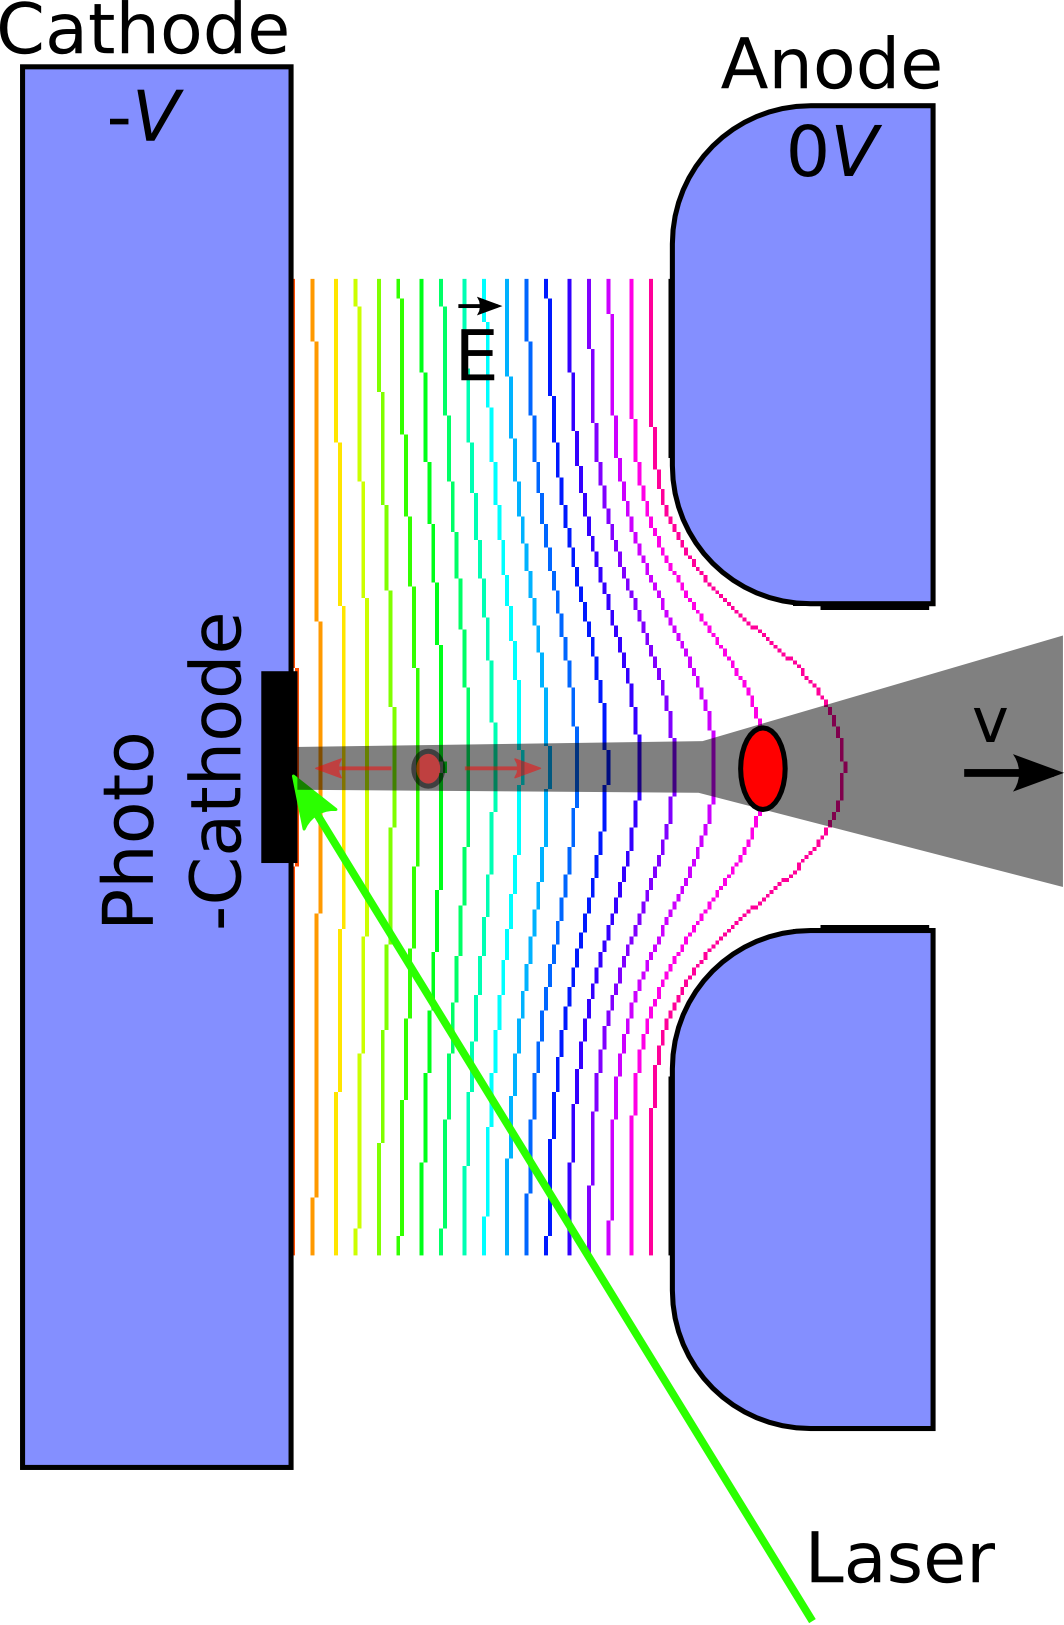
\includegraphics[width=0.5\linewidth]{acc_field}\\
      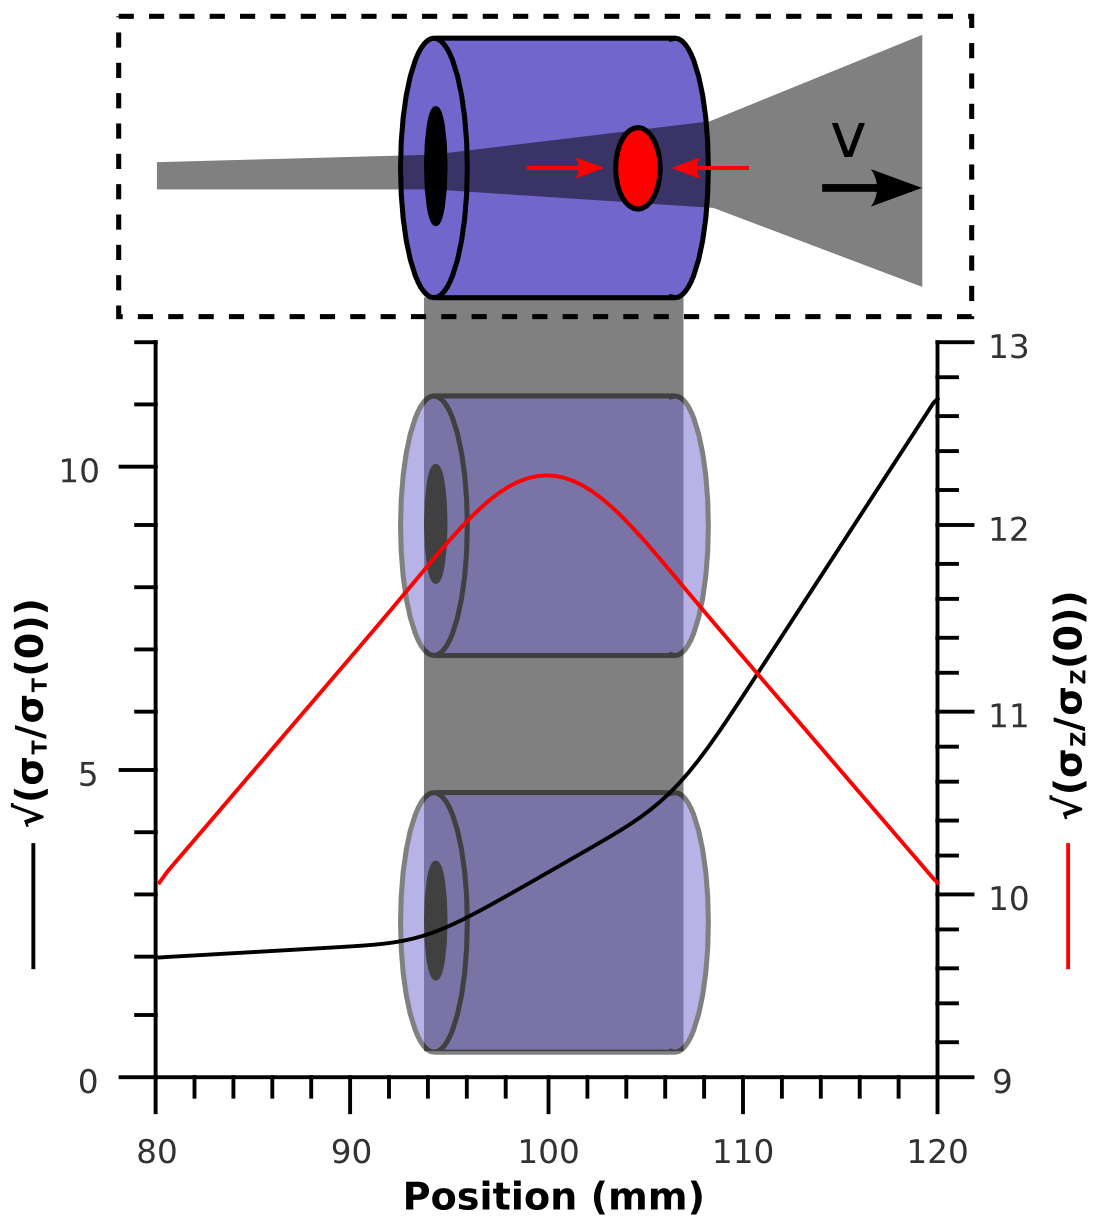
\includegraphics[width=0.5\linewidth]{RFCav}
    \end{figure}
  \end{column}
\end{columns}
\end{frame}

\begin{frame}{AG Model Example}
  \begin{center}
    %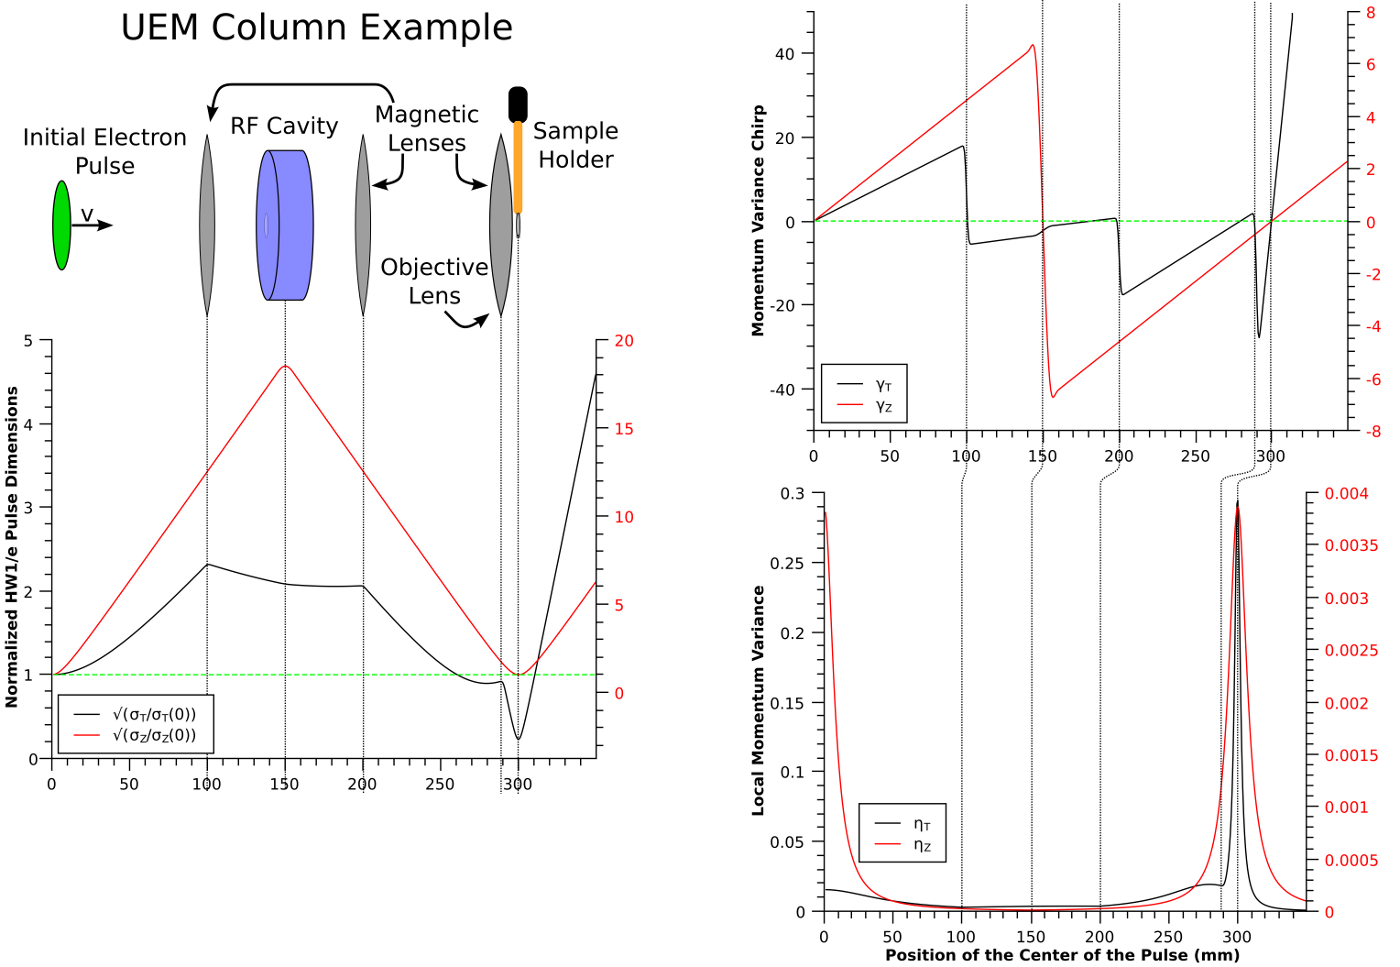
\includegraphics[width=0.7\linewidth]{Cooke_Column}
    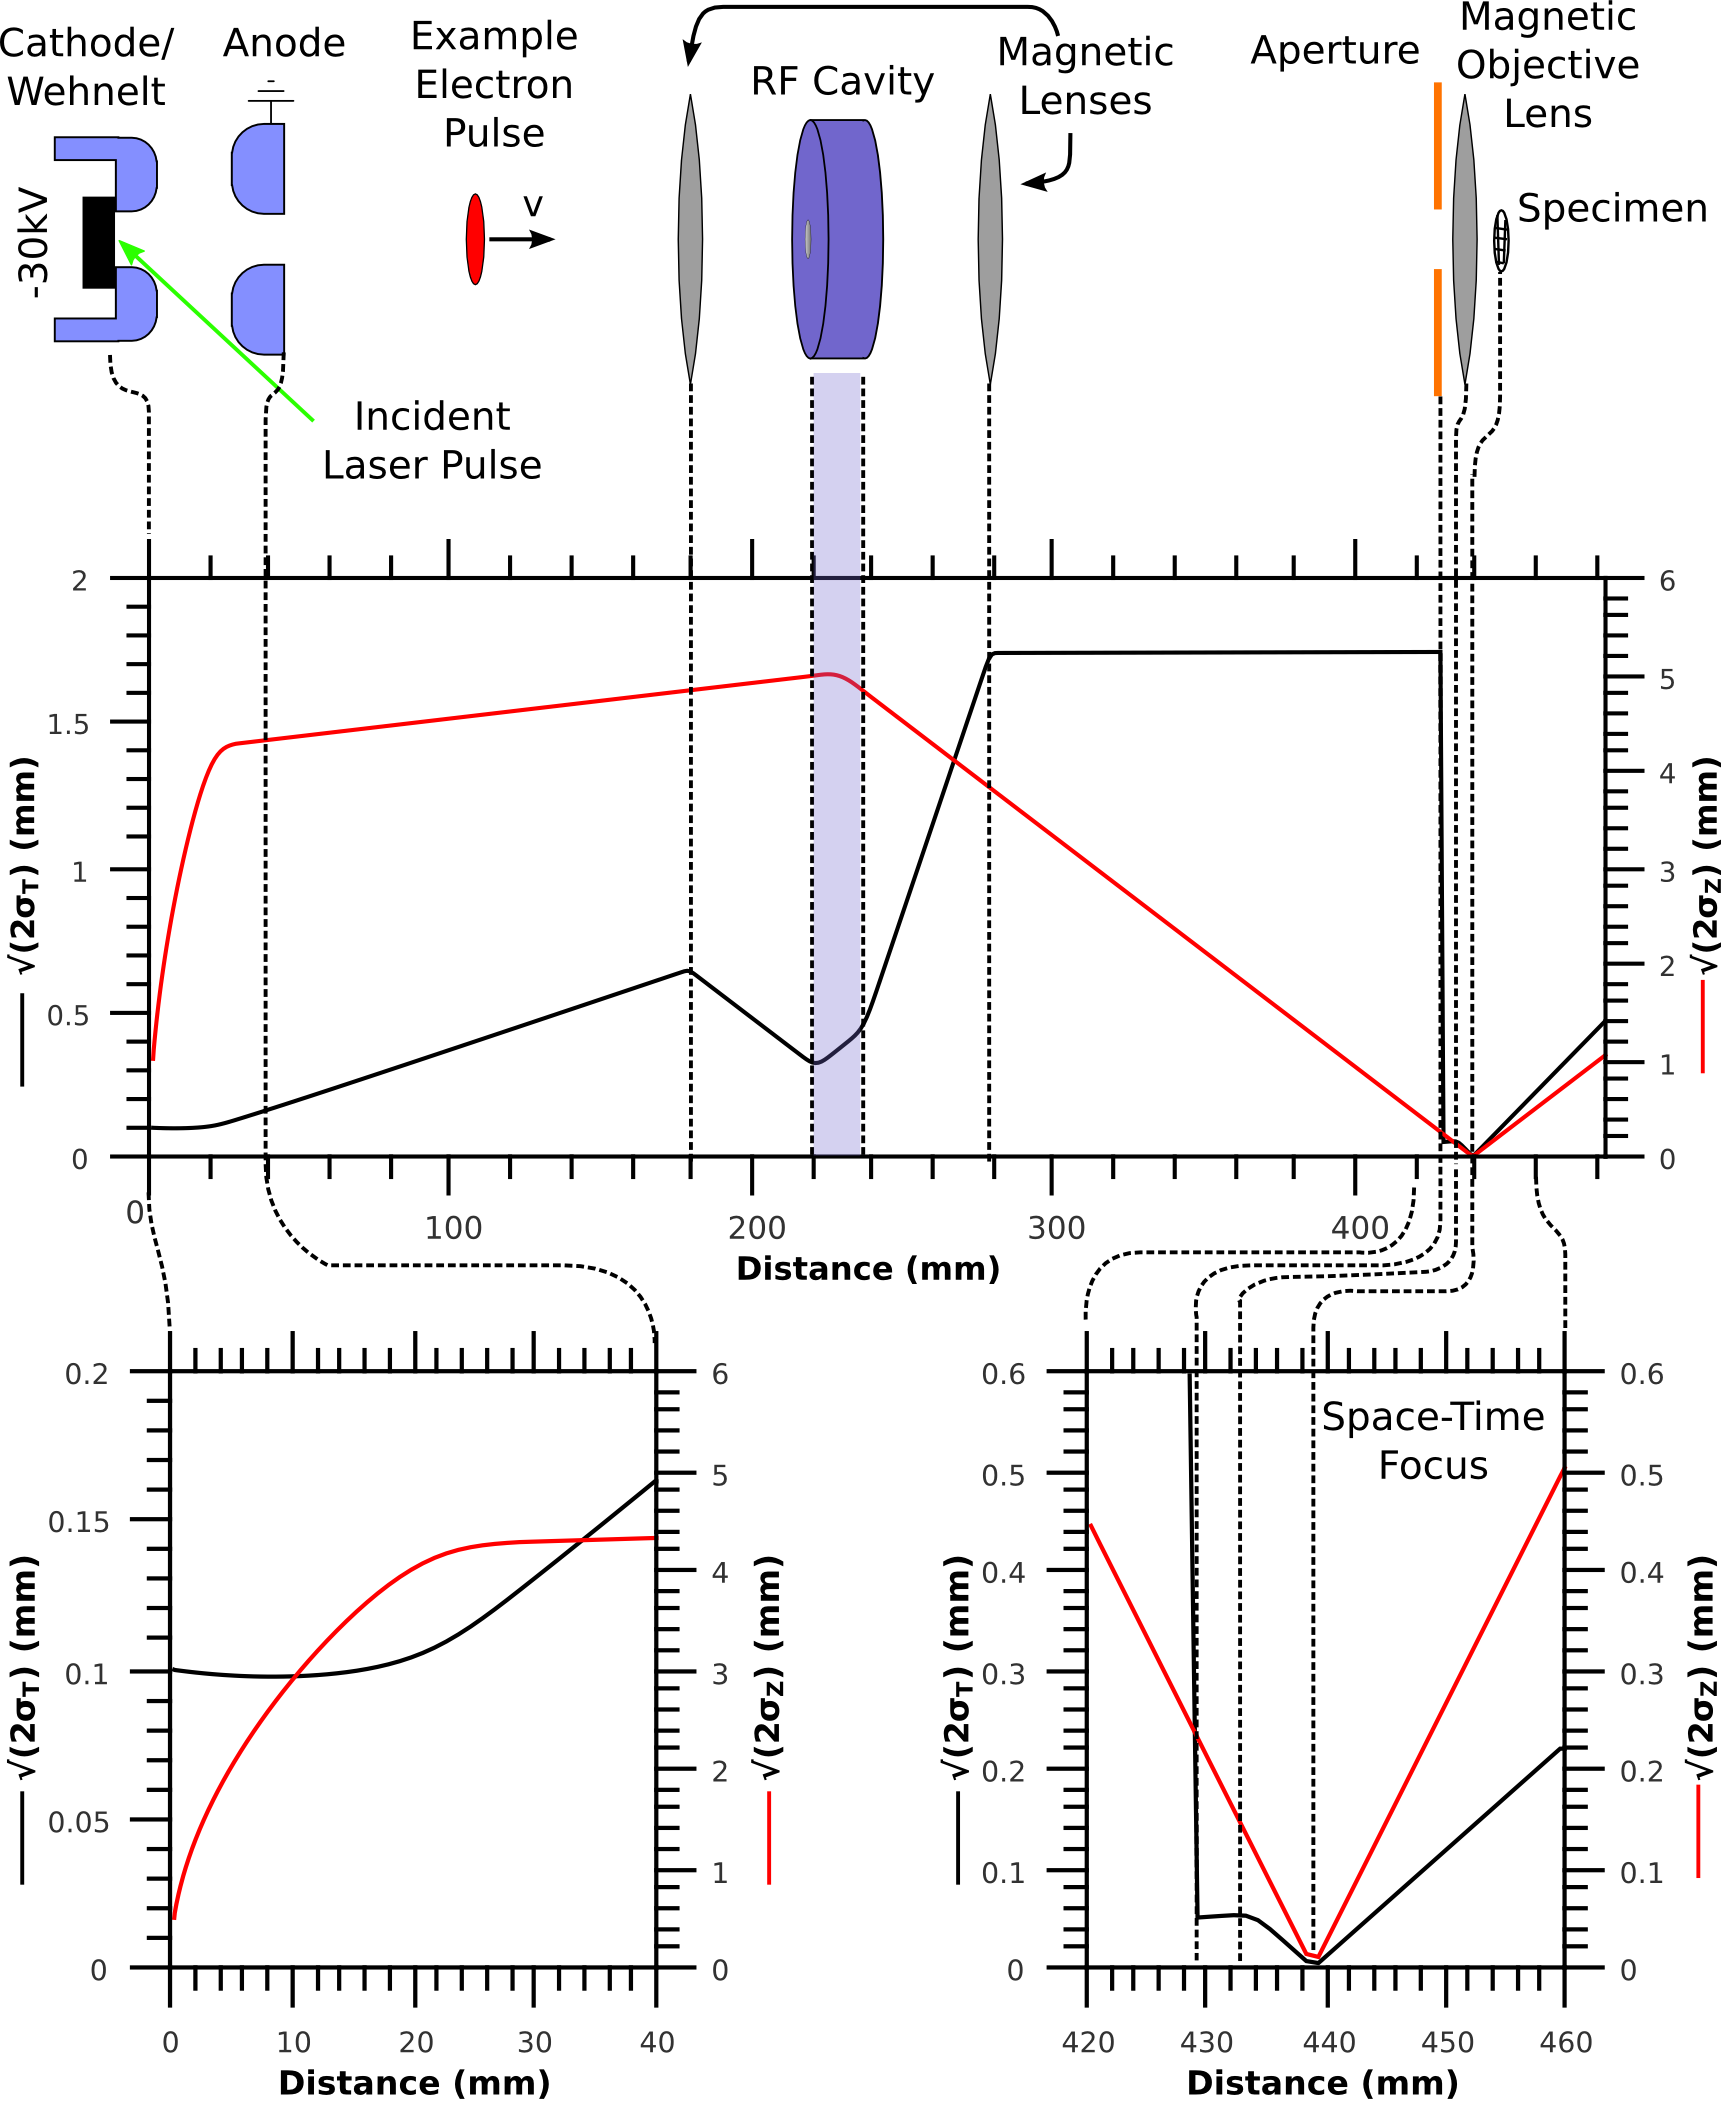
\includegraphics[width=0.5\linewidth]{Column}
  \end{center}
\end{frame}

\section{Future Work / Summary}

\begin{frame}{Future Work}
  \begin{block}{Ultrafast Group Goal}
    A novel UEM housed at UIC (Research Resources Center --- East) incorporating my laser-driven photogun
  \end{block}
  \begin{itemize}
    \item<2-> Investigate $m^{*}$ photoemission dependence
    \item<3-> Install RF compression cavity
    \item<4-> Devise and install pulse duration measurement
    \item<5-> Extend simulation for longer pulses and relativistic speeds
  \end{itemize}
\end{frame}

\begin{frame}{Summary}
Time Resolved Electron Microscopy is attempting to push time resolution to sub-ps time scales
  \begin{itemize}
    \item<2-> Highlighted several challenges including
    \begin{itemize}
      \item<2-> Difficulty generating short electron pulses of sufficient charge
      \item<3-> Necessity of generating low emittance pulses
      \item<4-> Difficulty maintaining the pulse integrity during propagation
      \item<5-> Need for useful simulations for optimization of columns
    \end{itemize}
    \item<6-> Demonstrated new techniques aimed at solving electron the pulse generation and delivery problem
    \begin{itemize}
      \item<7-> Nanopatterned photocathodes
      \begin{itemize}
        \item [$\hookrightarrow$] Plasmon-enhanced photoemission
      \end{itemize}
      \item<8-> Large aperture electron optical elements
      \item<9-> Column simulation based on AG model
    \end{itemize}
  \end{itemize}
\end{frame}

\begin{frame}{Thanks}
Thanks to:
\begin{columns}
  \begin{column}{.49\linewidth}
    \begin{itemize}
      \item Committee members
      \item Dept. of Energy (NNSA)
      \item National Science Foundation
      \item Argonne Nat'l Lab (FIB)
      \item Prof. W. Andreas Schroeder
      \item Ultrafast Group members
      \begin{itemize}
        \item Ben Rickman
        \item John Hogan
        \item Tuo Li
        \item Stephanie Schieffer\\(Air Force Research Lab)
      \end{itemize}
    \end{itemize}
  \end{column}

  \begin{column}{.49\linewidth}
    \begin{columns}
      \begin{column}{1in}
        \begin{figure}
          
\includegraphics[width=0.7in]{doe}
        \end{figure}
      \end{column}

      \begin{column}{1in}
        \begin{figure}
          
\includegraphics[width=0.7in]{nsf}
        \end{figure}
      \end{column}
    \end{columns}
    \vspace{0.4in}
    \begin{center}
      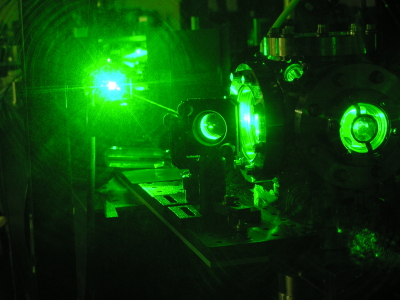
\includegraphics[width=1.3in]{Laser_Small}
    \end{center}
  \end{column}
\end{columns}
\end{frame}

%\appendix
%
\begin{frame}{Child-Langmuir Law}

\begin{columns}
  \begin{column}{0.45\linewidth}
    For two plates:
    \begin{itemize}
      \item area $A$
      \item separated by $d$
      \item potential difference $V_a$
    \end{itemize} the limiting current is given by:
  \end{column}
  \begin{column}{0.45\linewidth}
    \begin{figure}
      \centering
      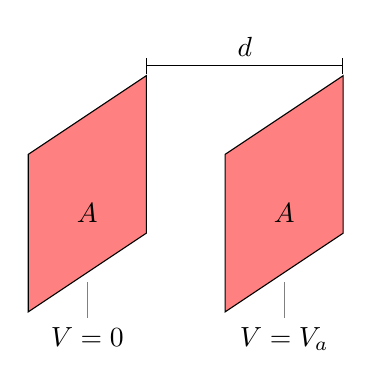
\begin{tikzpicture}
        \draw [fill=red!50]
          (0,0)
          -- node[below=1]{$A$}
            node(plate1)[above,pos=1]{}
            ++(1.5,1)
          -- ++(0,-2)
          -- node[pin={below:$V=0$}]{} ++(-1.5,-1)
          -- cycle
        ;
        \draw [fill=red!50]
          (2.5,0)
          -- node[below=1]{$A$}
            node(plate2)[above,pos=1]{}
            ++(1.5,1)
          -- ++(0,-2)
          -- node[pin={below:$V=V_a$}]{} ++(-1.5,-1)
          -- cycle
        ;
        \draw[|-|]
          (plate1.center)
          -- node[above]{$d$} (plate2.center);
      \end{tikzpicture}
    \end{figure}
  \end{column}
\end{columns}
\begin{block}{Child-Langmuir Law}
  \begin{equation*}
    I_a  = JA = \frac{4 \varepsilon_0}{9}\sqrt{\frac{2 e}{m_e} } \frac{A V_a^{3/2}}{d^2}
  \end{equation*}
\end{block}
\end{frame}

\begin{frame}{Quantum Step Approximation}
	\begin{columns}
	\begin{column}{.48 \linewidth}
    We have the relations:
    	\begin{itemize}
          \item $ k_{0 \smallT} = k_{1 \smallT} $
          \item<2-> Trigonometric Identities
          \item<3-> 1D Transmission result: \\ $ T(k(E),\theta) =
          \frac{4 k_{0 z} k_{1 z}}{ \left ( k_{0 z} + k_{1 z} \right ) ^{2} } $
        \end{itemize}    
  	\end{column}
	\begin{column}{.52 \linewidth}
    	\begin{figure}[H]
          	\centering
        	\shadowbox
        	{
        	\only<article| beamer>{
        	\only<1-3>{
        	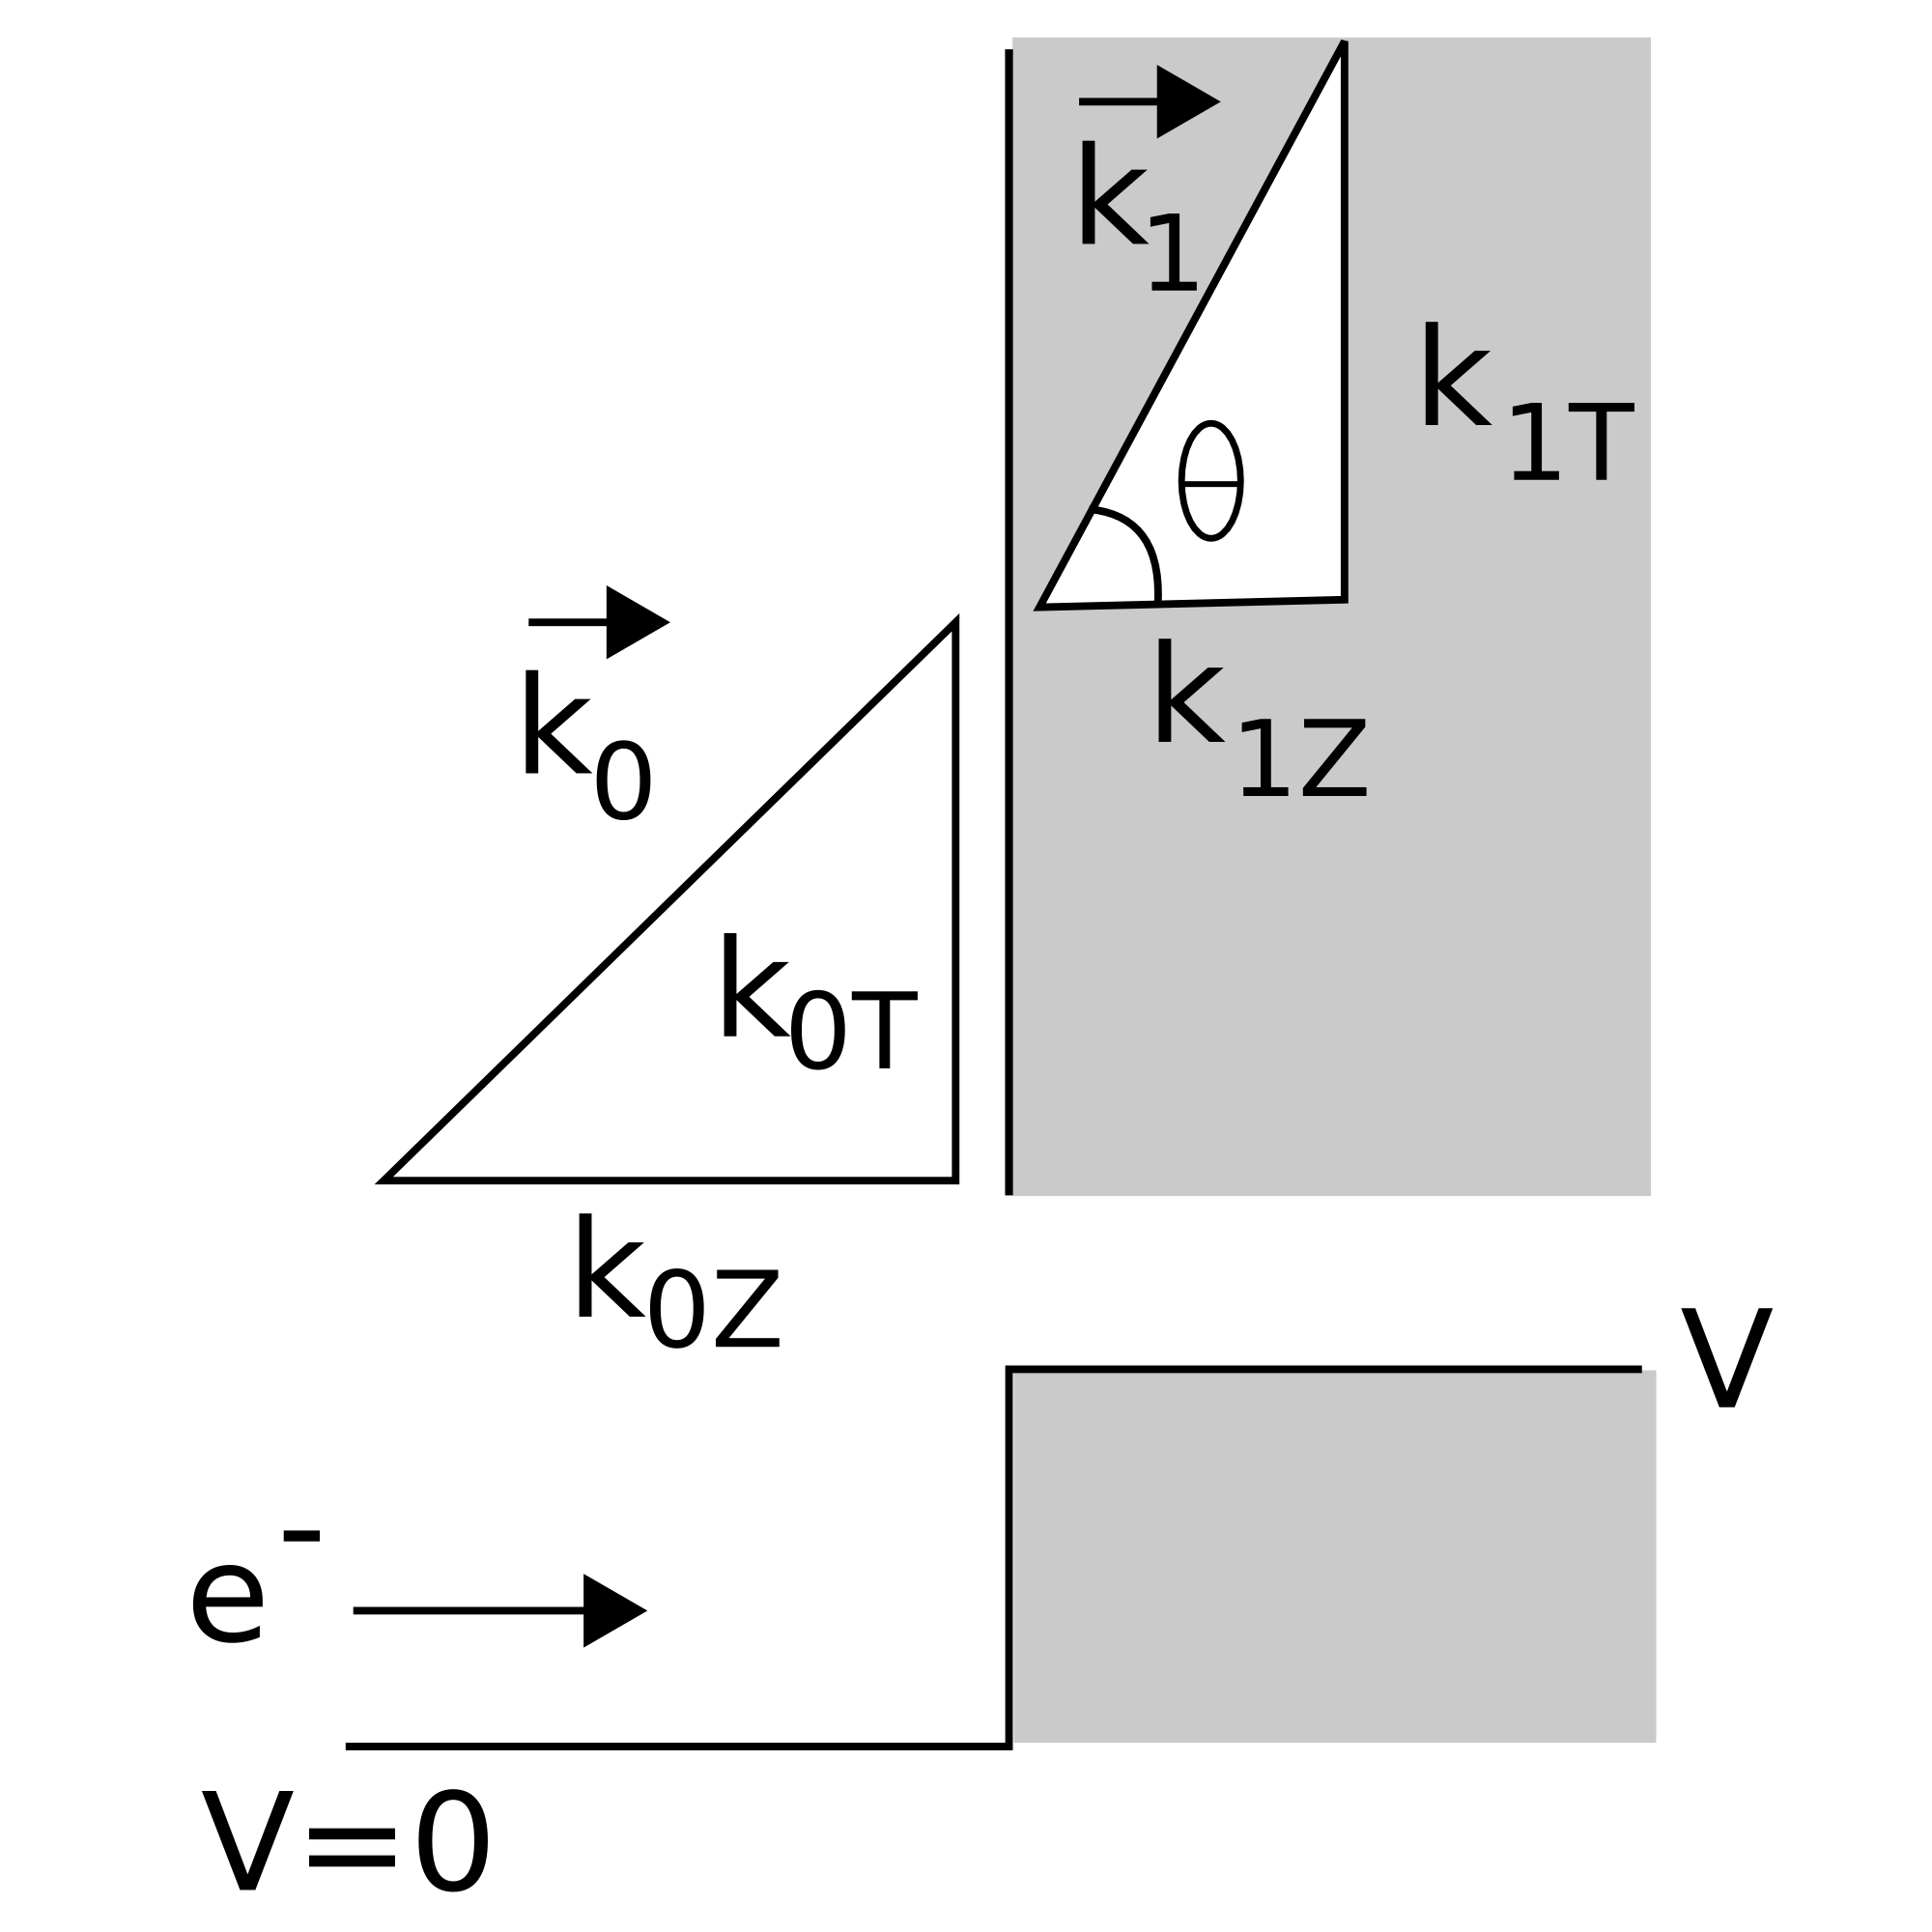
\includegraphics{quantum_step}
        	}}
        	\only<presentation>{
        	\only<4->{
        	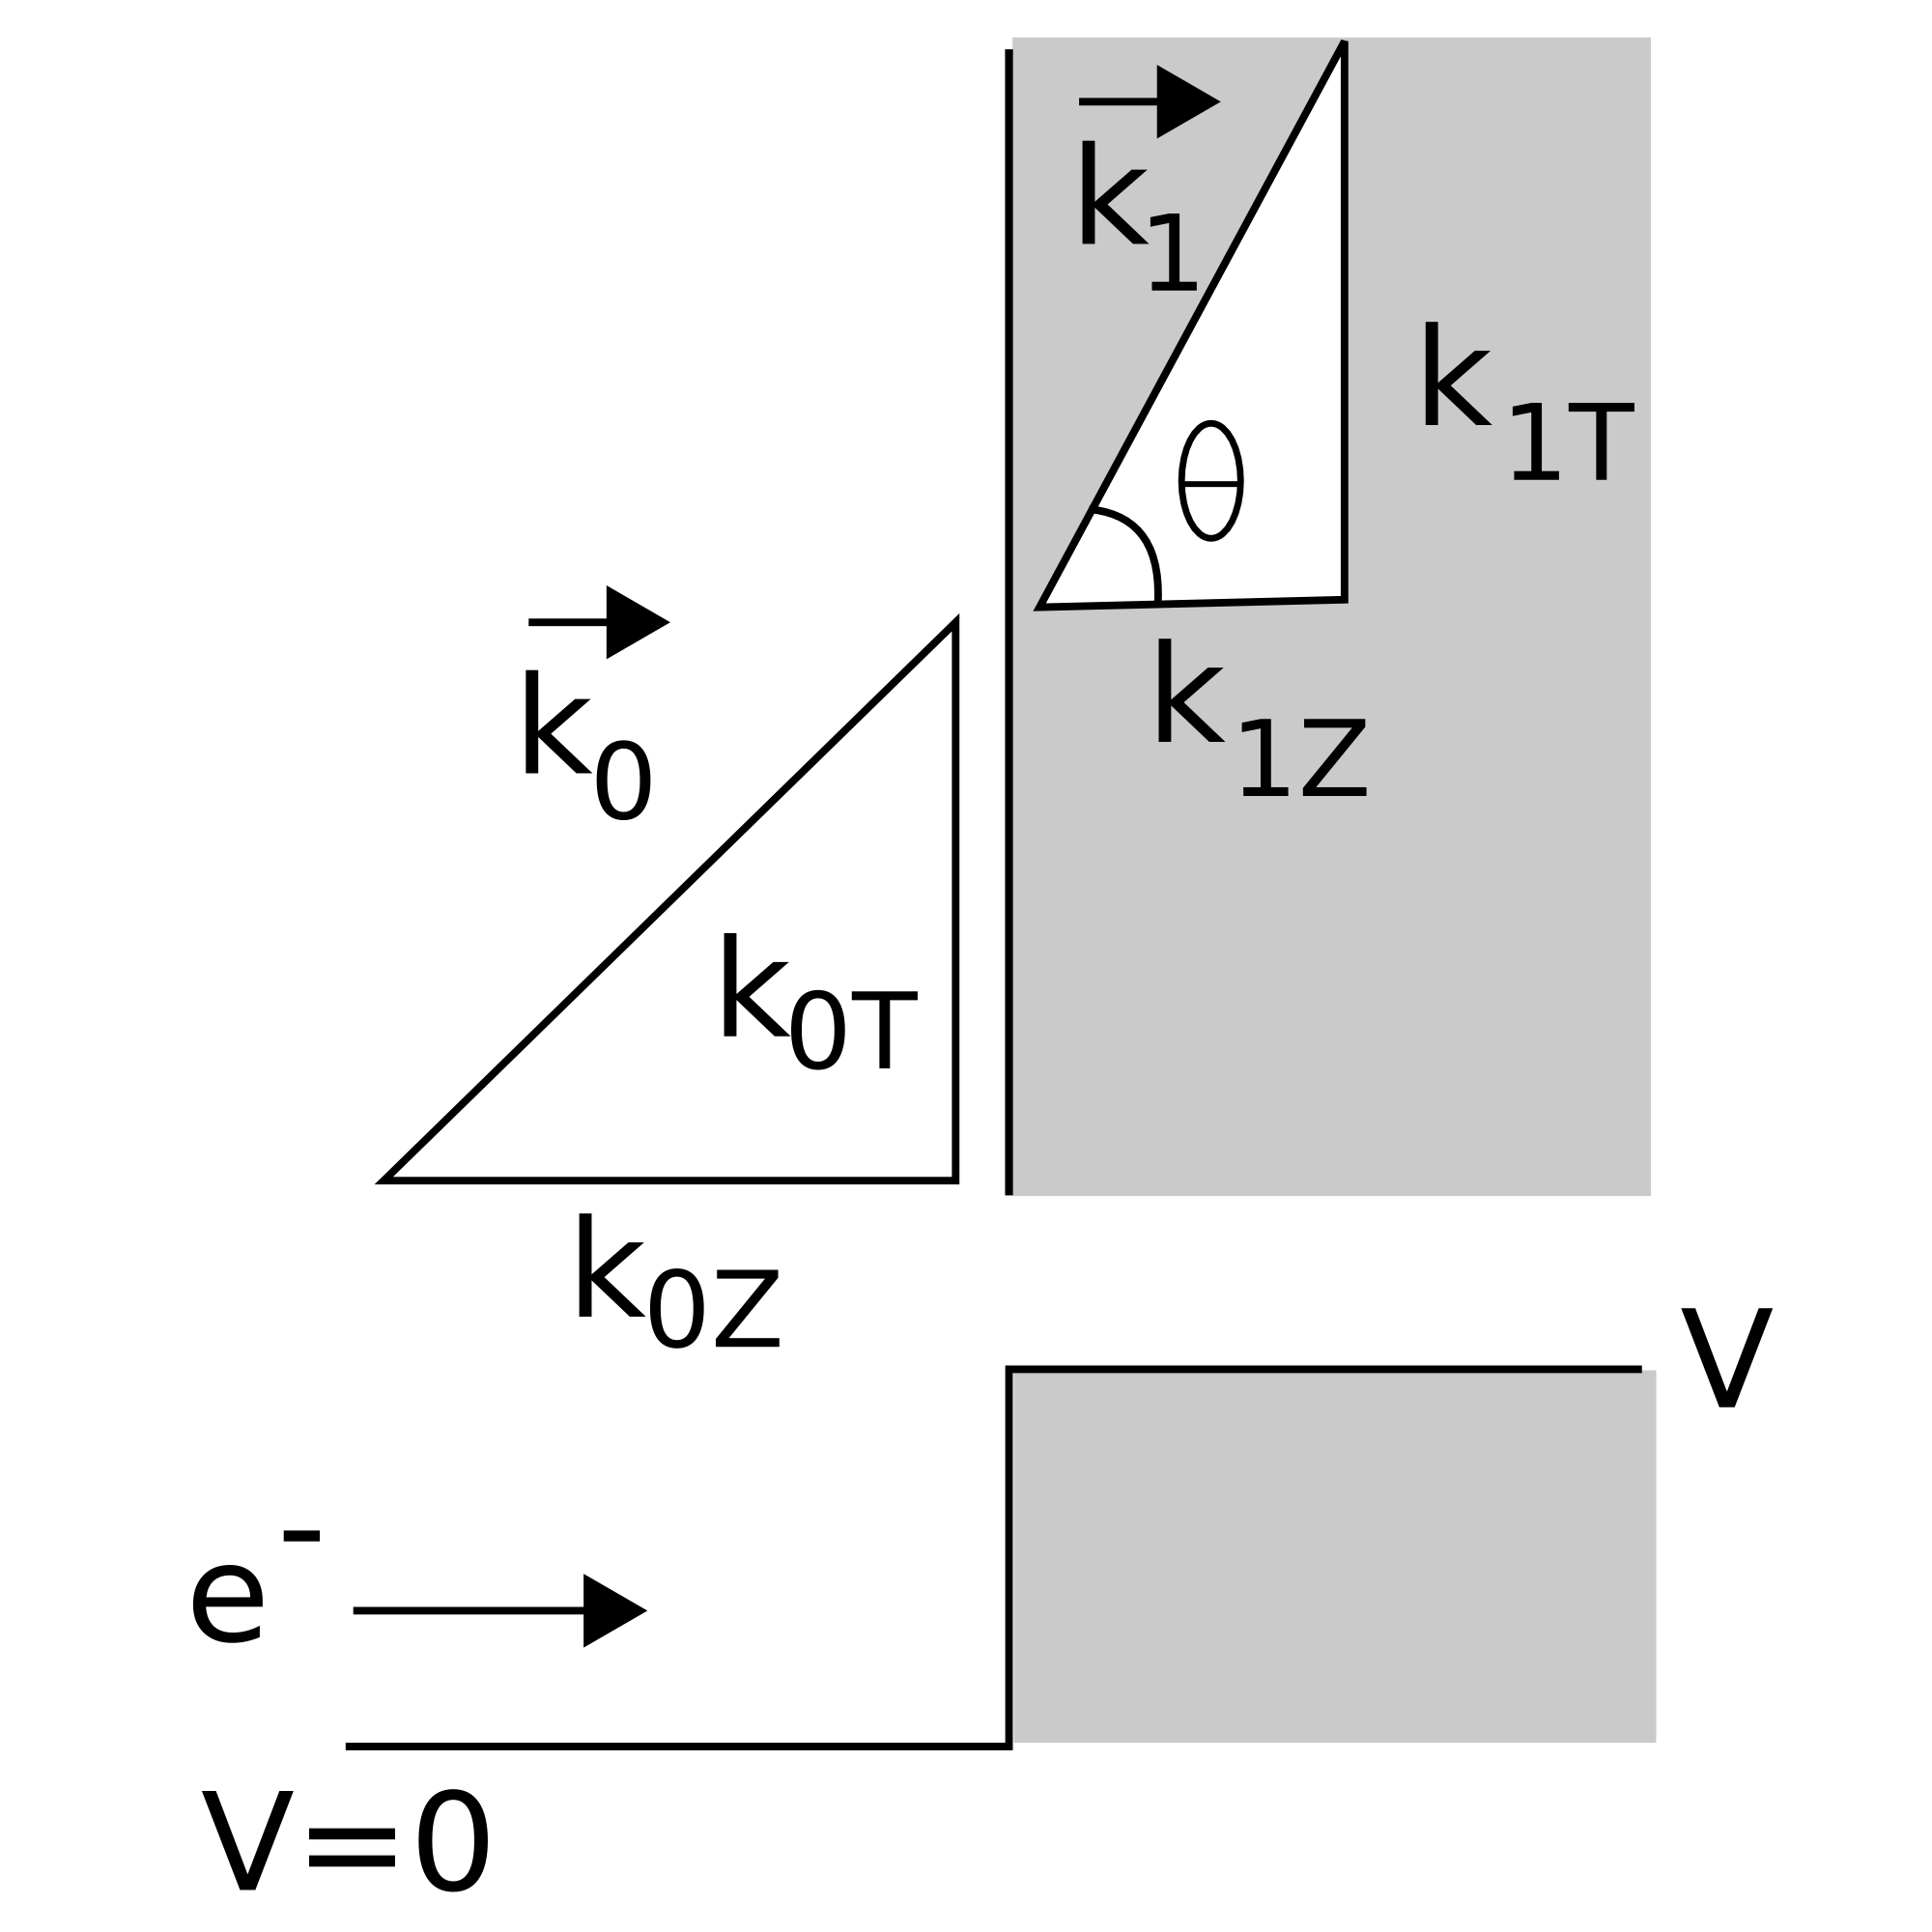
\includegraphics[scale=0.7]{quantum_step}}
        	}}
        	\only<article>{\caption{Quantum Step Potential}}
        \end{figure}
    \end{column}
	\end{columns}
\only<4->
{
    \begin{block}{Resulting Transmission Function}
        \begin{equation*}
           	T(E,\theta) = \frac{4 \sqrt{E} \cos \theta \sqrt{E \cos^{2} \theta
           	+ V } }{ \left ( \sqrt{E} \cos \theta + \sqrt{E \cos^{2} \theta
           	+ V } \right )^{2} }
    	\end{equation*}
		\center{In terms of exit energy $E$ and exit angle $\theta$}
    \end{block}
}
\end{frame}

\begin{frame}{Photoemission from Flat Metal}
  \begin{columns}
  \begin{column}{0.54\linewidth}
  \begin{center}
  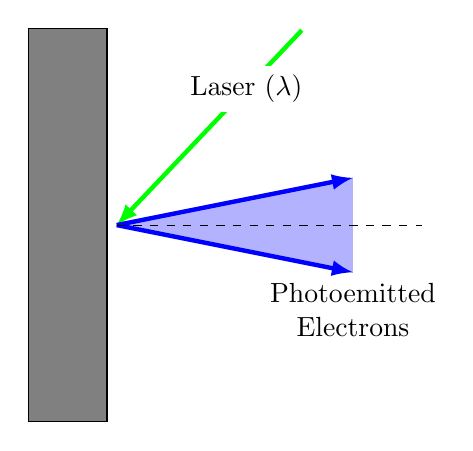
\begin{tikzpicture}
    \filldraw
      [fill=black!50]
      (0,0) 
      node [name=photocathode1,below right]{}
      node [below=1mm of photocathode1] {}
      -- ++(1,0)
      -- ++(0,-5)
      node [name=source,midway] {} 
      -- ++(-1,0)
      -- cycle
    ;
    \draw
      [-latex,ultra thick,green] 
      ($(source) + (45:3.5)$) 
      -- (source.east)
      node [name=laser label,pos=0.3,black,fill=white] {Laser ($\lambda$)}
    ;
    \fill
      [blue!30]
      (source.east)
      -- ++(3,6mm)
      -- ++(0,-12mm)
      -- cycle
    ;
    \draw
      [-latex,ultra thick,blue]
      (source.east)
      -- ++(3,6mm)
    ;
    \draw
      [-latex,ultra thick,blue]
      (source.east)
      -- ++(3,-6mm)
      node [name=electron label,at end,black,below,align=center]{Photoemitted\\Electrons}
    ;
    \draw
      [dashed]
      (source)
      -- ++(4,0)
    ;
%     \draw 
%       ($(source) + (1,0)$) 
%       arc (0:41:1)
%       node [right=0.3] {$\theta$}
%     ;
  \end{tikzpicture}
  \end{center}
  \end{column}
  \begin{column}{0.44\linewidth}
    \begin{equation*}
      P(\theta) = \smashoperator{\int\limits_{0}^{\Delta E = \hbar \omega - \Phi}} T(E,\theta) \dx{E}
    \end{equation*}
    \centerline{\tiny Assuming flat fermi function}
    \begin{figure}
      \centering
      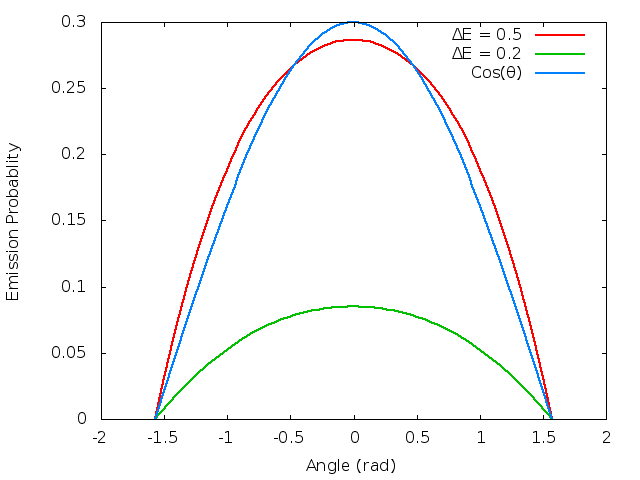
\includegraphics[width=0.9\linewidth]{Angle}
    \end{figure}
  \end{column}
  \end{columns}
\end{frame}

\begin{frame}{Emission Probability vs. Excess Energy}
  \begin{columns}
    \begin{column}{0.49\linewidth}
      %Angularly-integrated Emission Probability
      \begin{equation*}
        P(E) = \int\limits_0^E \int\limits_{-\pi/2}^{-\pi/2} T(E_0,\theta) \dx{\theta}\dx{E_0}
      \end{equation*}
    \end{column}
    \begin{column}{0.49\linewidth}
      \begin{figure}
        \centering
        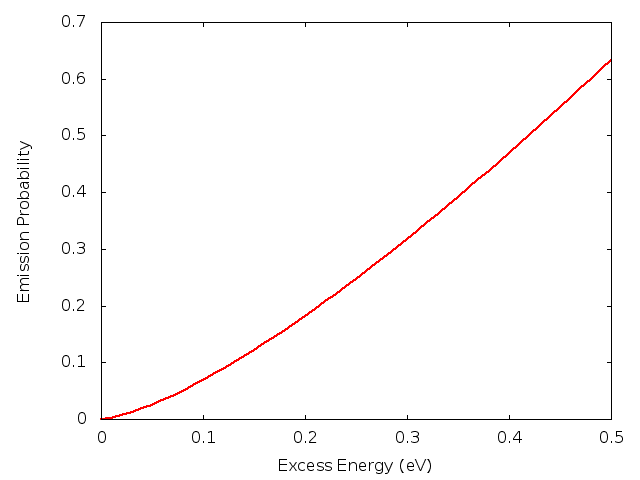
\includegraphics[width=0.9\linewidth]{Energy}
      \end{figure}
    \end{column}
  \end{columns}
  
\end{frame}

\begin{frame}{Gaussian Distribution}
If we define our distribution of electrons in the pulse as:
	\begin{multline*}
		f \left ( x , y , z , p_{x} , p_{y} , p_{z} \right ) = \\ \frac{N}{ \left ( 2 \pi \right )^{3} \sigma_{ \smallT } \eta_{ \scriptscriptstyle T } \sqrt{ \sigma_{z} \eta_{z}} } \exp \Biggl [ - \biggl ( \frac{x^{2}} {2 \sigma_{ \smallT }} + \frac{y^{2}} {2 \sigma_{ \smallT }} + \frac{z^{2}} {2\sigma_{z}} + \\ \frac{ \left ( p_{x} - \dfrac{\gamma_{ \smallT } x} {\sigma_{ \smallT }} \right )^{2}} {2 \eta_{ \smallT }} + \frac{ \left ( p_{y} - \dfrac{\gamma_{ \smallT } y} {\sigma_{ \smallT }} \right )^{2}} {2 \eta_{ \smallT }} + \frac{ \left (p_{z} - \dfrac{\gamma_{z} z} {\sigma_{z}} \right )^{2}} {2 \eta_{z}} \biggr ) \Biggr ]
	\end{multline*}
N.B. the coefficient allows $ \int f d\vec{r} d\vec{p} = N $

\end{frame}

\begin{frame}{What Are These Parameters?}
	\begin{columns}
		\begin{column}{2in}
			\begin{itemize}[<+->]
				\item $ \sigma_{i} \Rightarrow$ spatial variance
				\item $ \eta_{i} \Rightarrow$ \emph{local} momentum variance
				\item $ \gamma_{i} \Rightarrow$ spatial variation of the local momentum variance (chirp)
			\end{itemize}
		\end{column}
		\begin{column}{2in}
			\begin{figure}
				\includegraphics<1>{Gaussian1.jpg}
				\includegraphics<2>{Gaussian2.jpg}
				\includegraphics<3>{Gaussian3.jpg}
			\end{figure}
		\end{column}
	\end{columns}
\end{frame}

\begin{frame}{AG Model Equations}
\begin{block}{Michalik and Sipe equation set}
	\begin{gather*}
		\frac{d\sigma_{i}} {dt} = \frac{2} {m} \gamma_{i} \\
		\frac{d \gamma_{i}} {dt} = \frac{1} {m} \left (\eta_{i} + \frac{\gamma_{i}^{2}} {\sigma_{i}} \right ) + \frac{1} {4 \pi \epsilon_{0}} \frac{N e^{2}} {6 \sqrt{\sigma_{i} \pi} } L_{i}(\xi) \\
		\frac{d\eta_{i}} {dt} = - \frac{2 \gamma_{i} \eta_{i}} {m \sigma_{i}}
	\end{gather*}
\end{block}
\begin{itemize}
  \item $L_i(\xi)$ are well-behaved smooth functions of $\xi=\sqrt{ \sigma_{z} / \sigma_{t} }$
  \item Solve to classical Gaussian when $ N = 0 $
\end{itemize}
\end{frame}

\begin{frame}{Building the Model}

\begin{columns}
	\begin{column}{.52 \linewidth}
	\begin{itemize}
  		\item<1-> Start with the fastest electron
  		\item<2-> $ v_{fastest} = \sqrt{2 q \Delta E / m } $ \\ $ \Delta E $ is
  		excess photoemission energy
  		\item<3-> Propagate with \\ $ z_{max} = v_{fastest} t_{total} + q E t_{
  		total }^{2} / 2 m $
  		\item<4-> This is the maximum possible range
  		\item<5-> Subdivide the preceding space for future reference
	\end{itemize}
	\end{column}
	
	\begin{column}{.44 \linewidth}
    \begin{overlayarea}{.44 \linewidth}{2.1in}
    \begin{figure}[H]
    	\centering
    	\only<beamer>
    	{
    	\only<1-2>{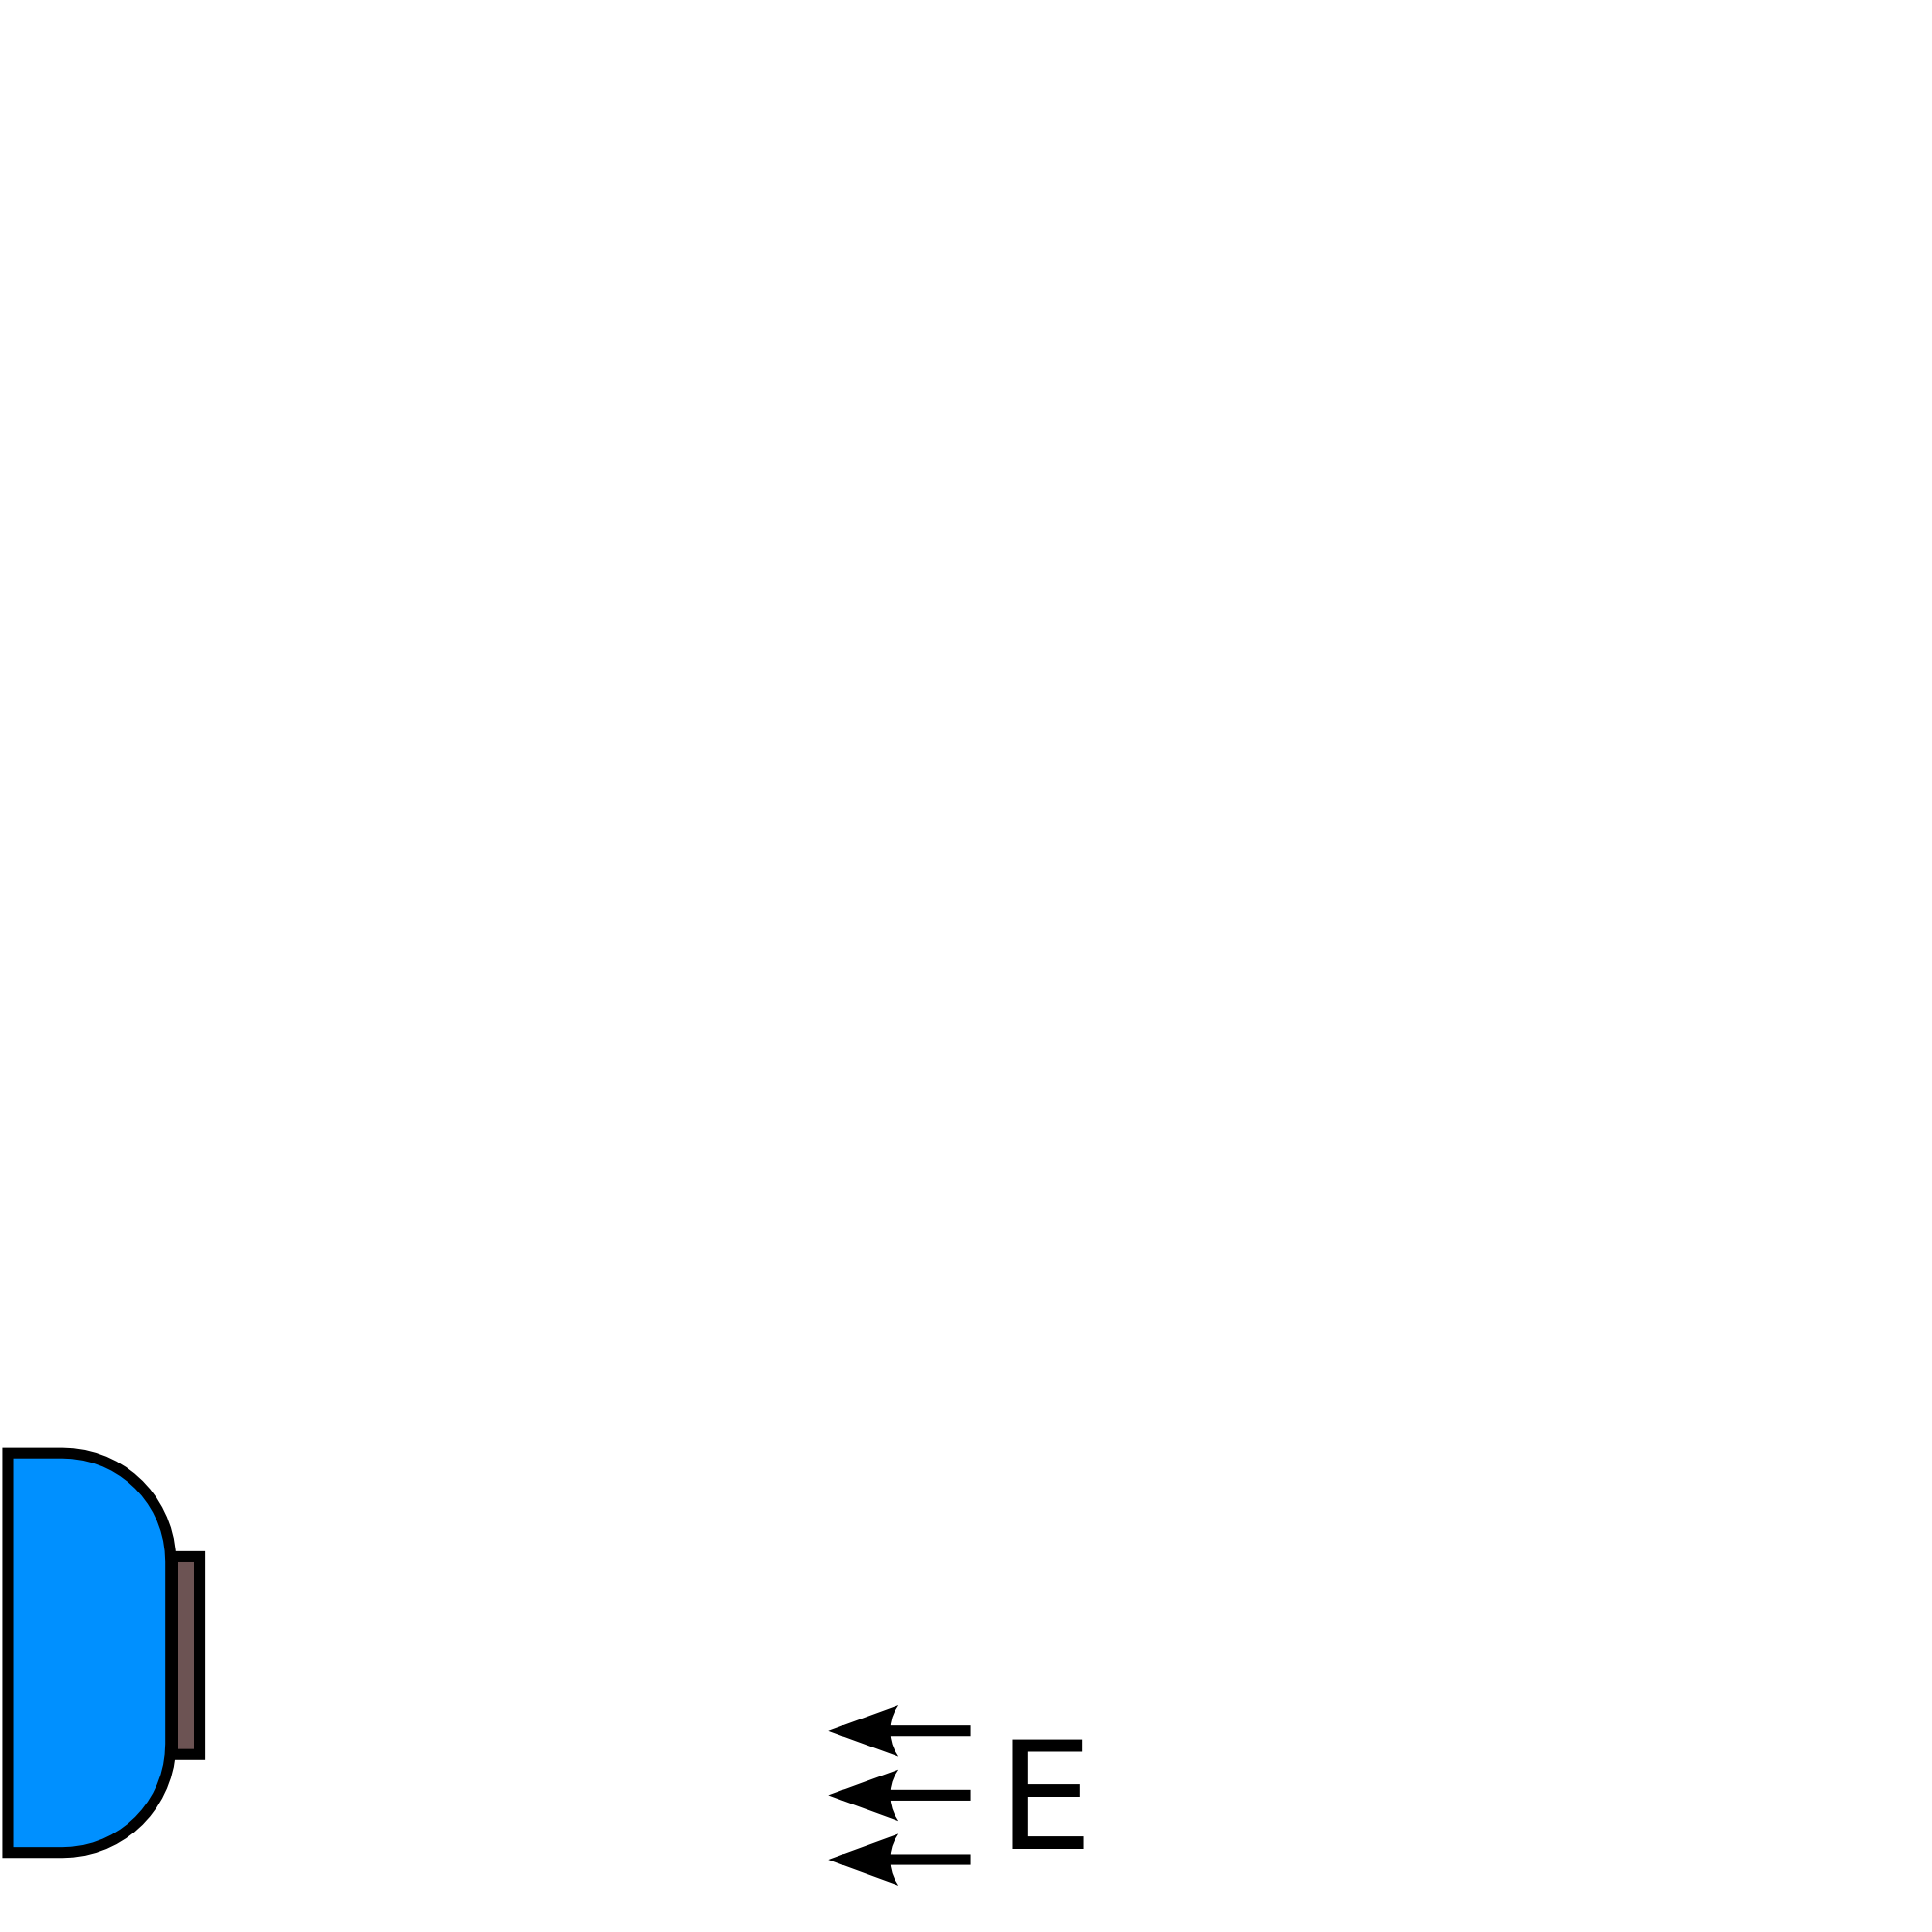
\includegraphics{bin}}
    	\only<3-4>{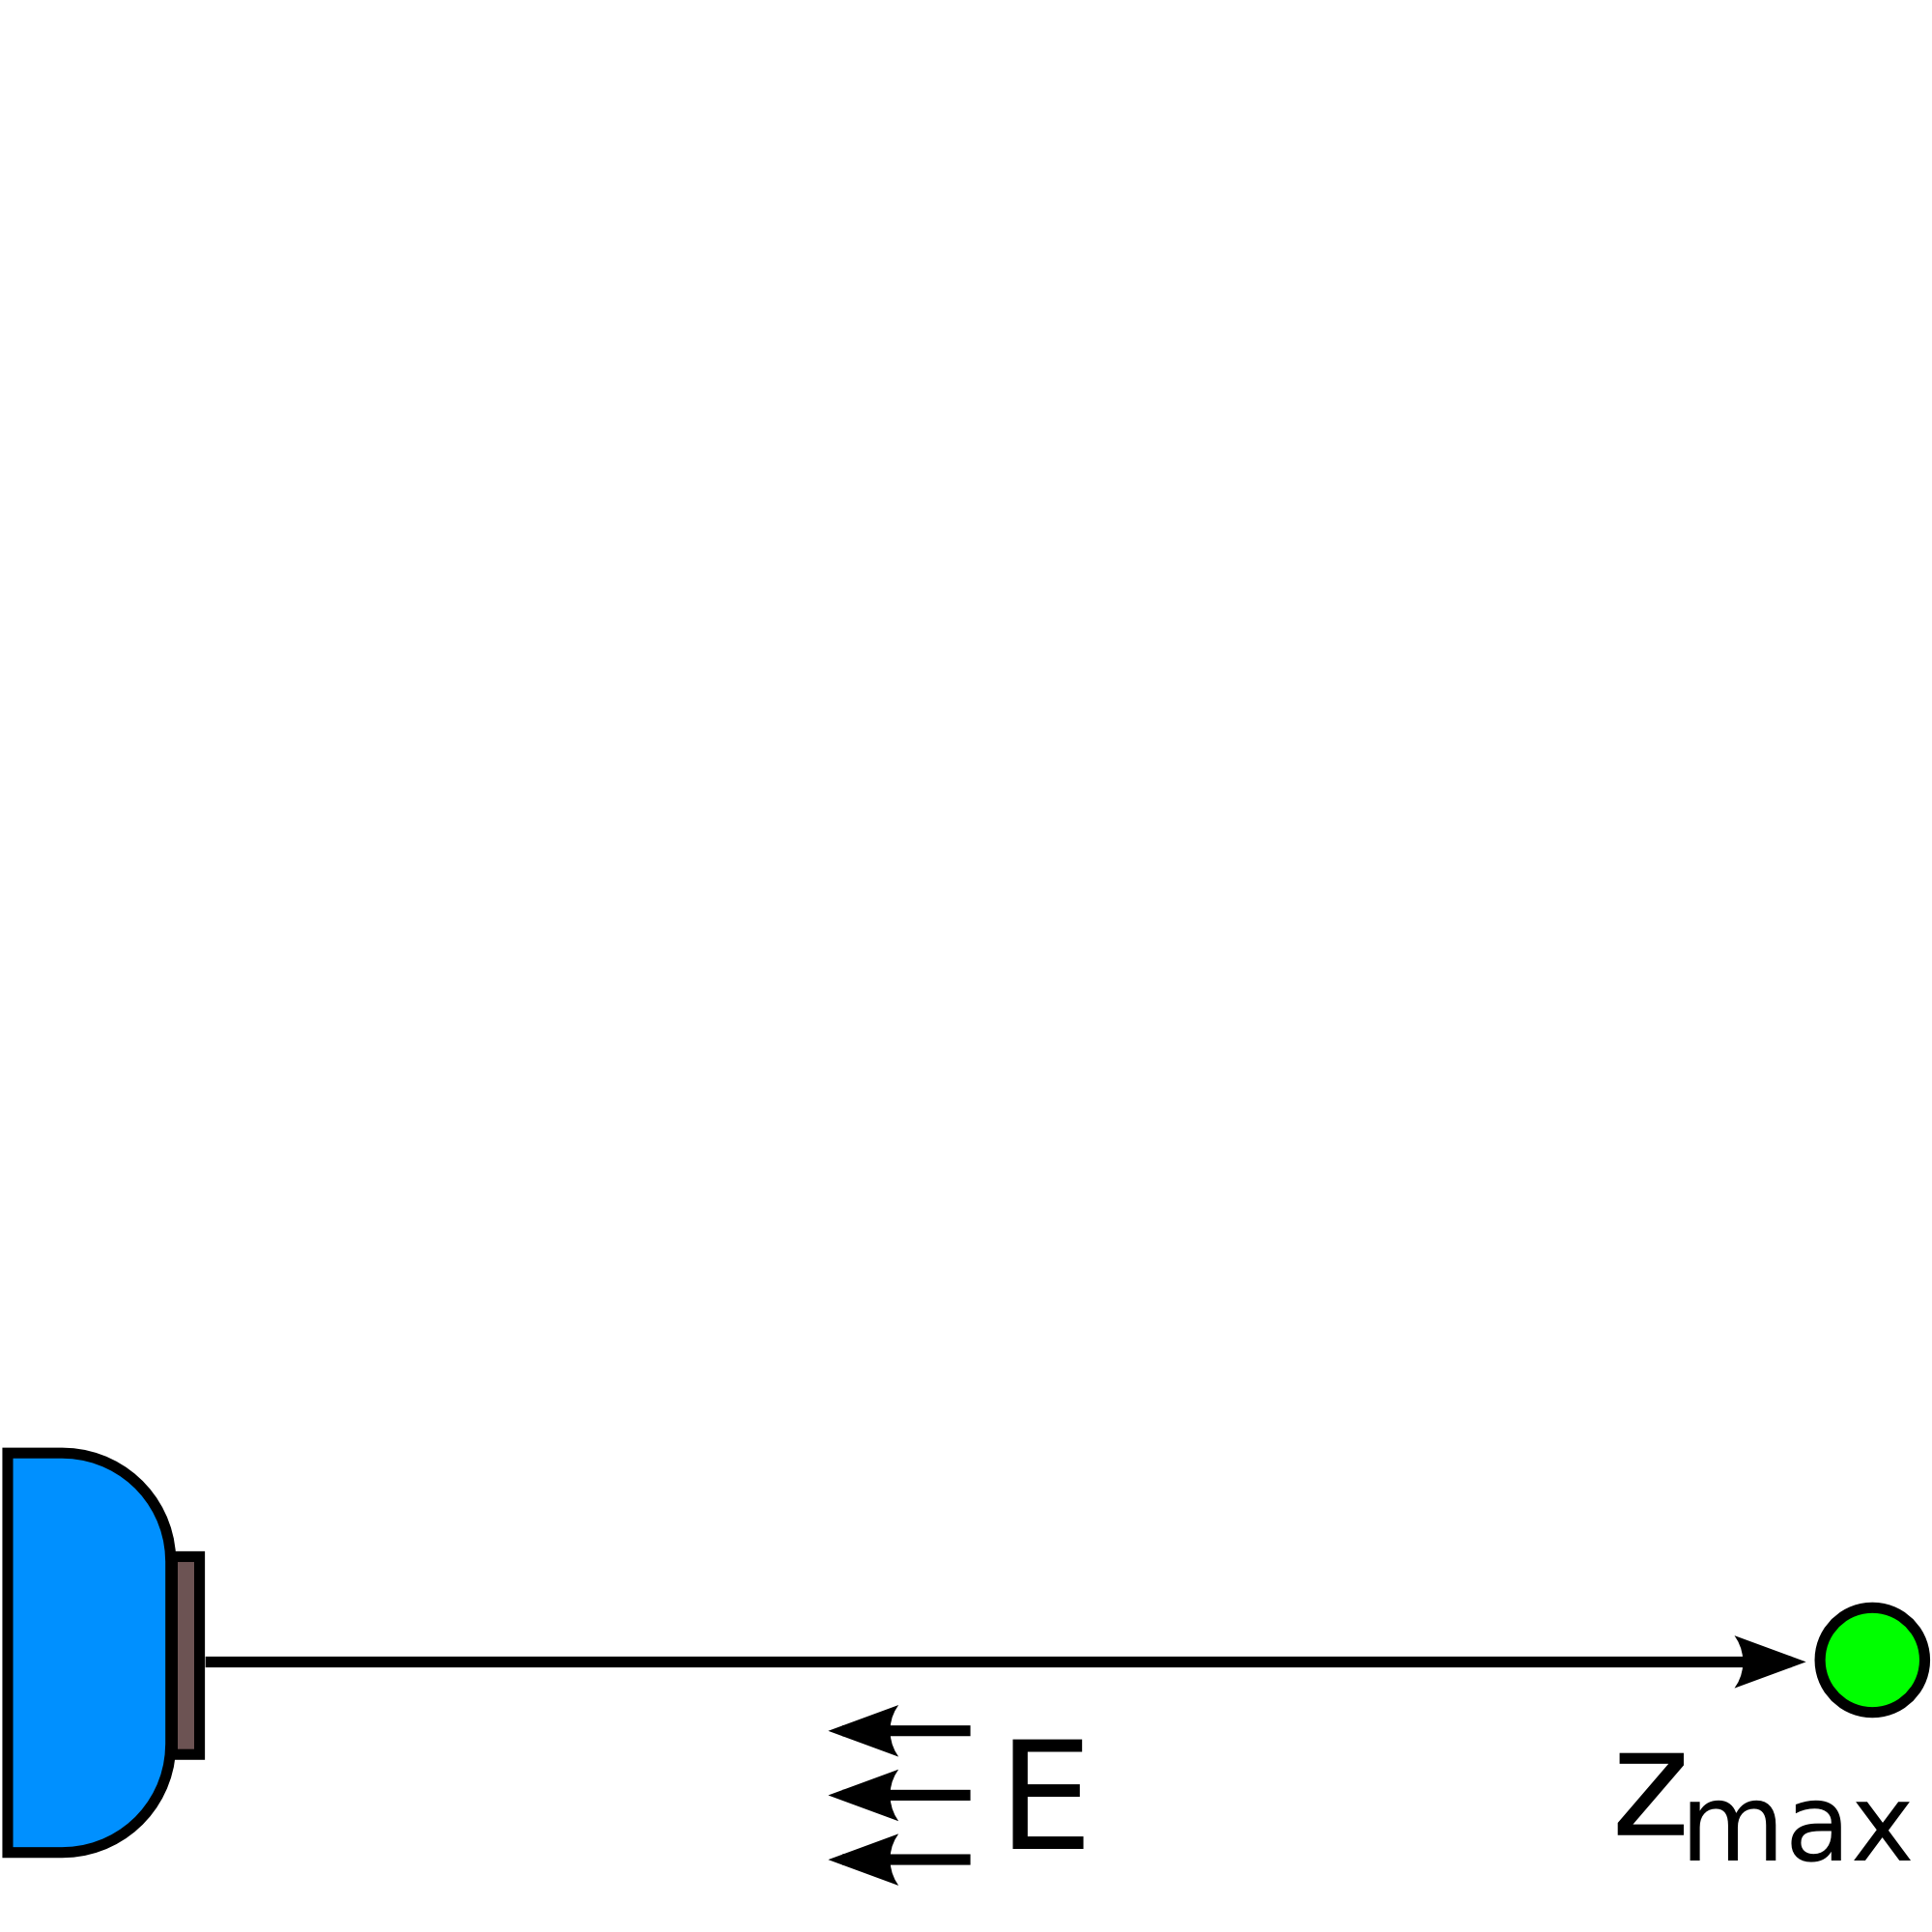
\includegraphics{bin1}}
    	}
    	\only<presentation>{\only<5->{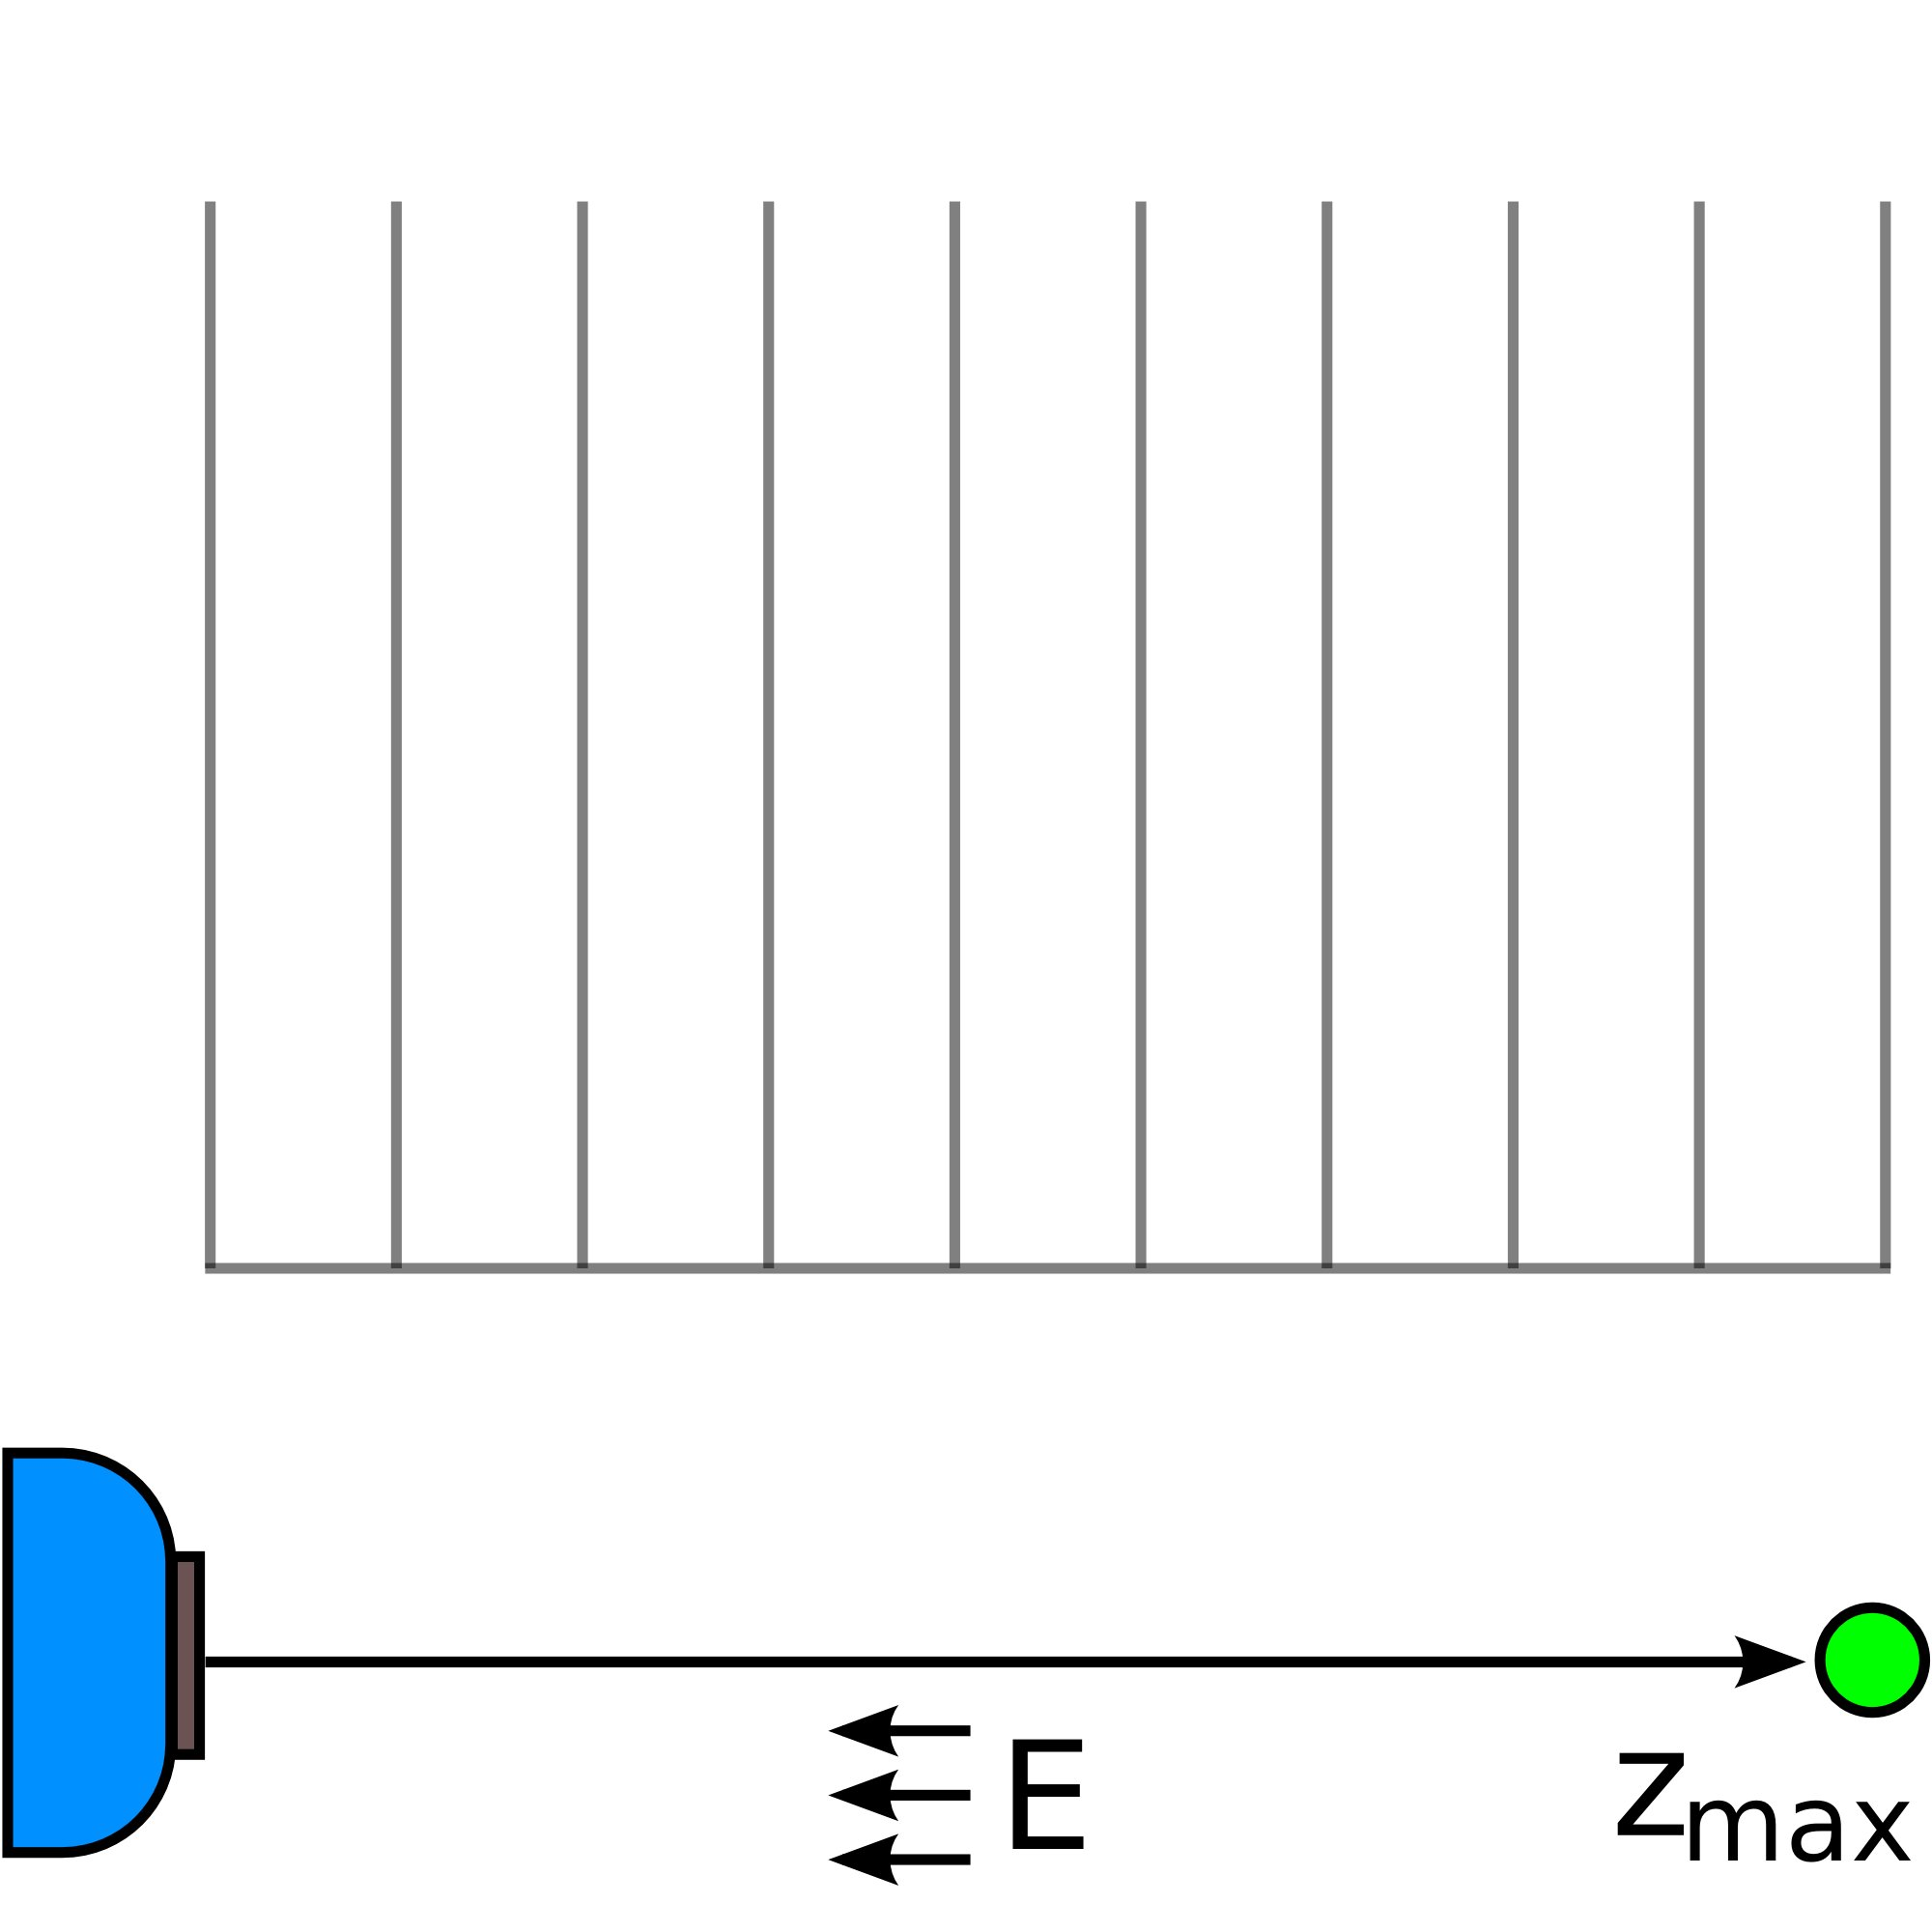
\includegraphics{bin2}}}
    \end{figure}
    \end{overlayarea}
    \end{column}
\end{columns}

\end{frame}

\begin{frame}{Running the Model}

\begin{columns}
	\begin{column}{.52 \linewidth}
	\begin{itemize}
      \item<1-> At each timestep $t_{i}$ label bins by equivalent velocities
      \item<2-> $ v_{ bin } = \frac{ z_{ bin } }{ t_{ i } } - \frac{q E t_{i} }{
      2 m } $ \\ where $ t_{i} =  t_{ total } - i \delta t $
      \item<3-> This allows the velocity distribution to be superimposed
      \item<10-> After all the timesteps the number and velocity distribution
      in each bin can be computed
    \end{itemize}
	\end{column}

	\begin{column}{.44 \linewidth}
    \begin{overlayarea}{.44 \linewidth}{2.1in}
	\begin{figure}[H]
    	\centering
    	\only<beamer>
    	{
    	\only<1-2>{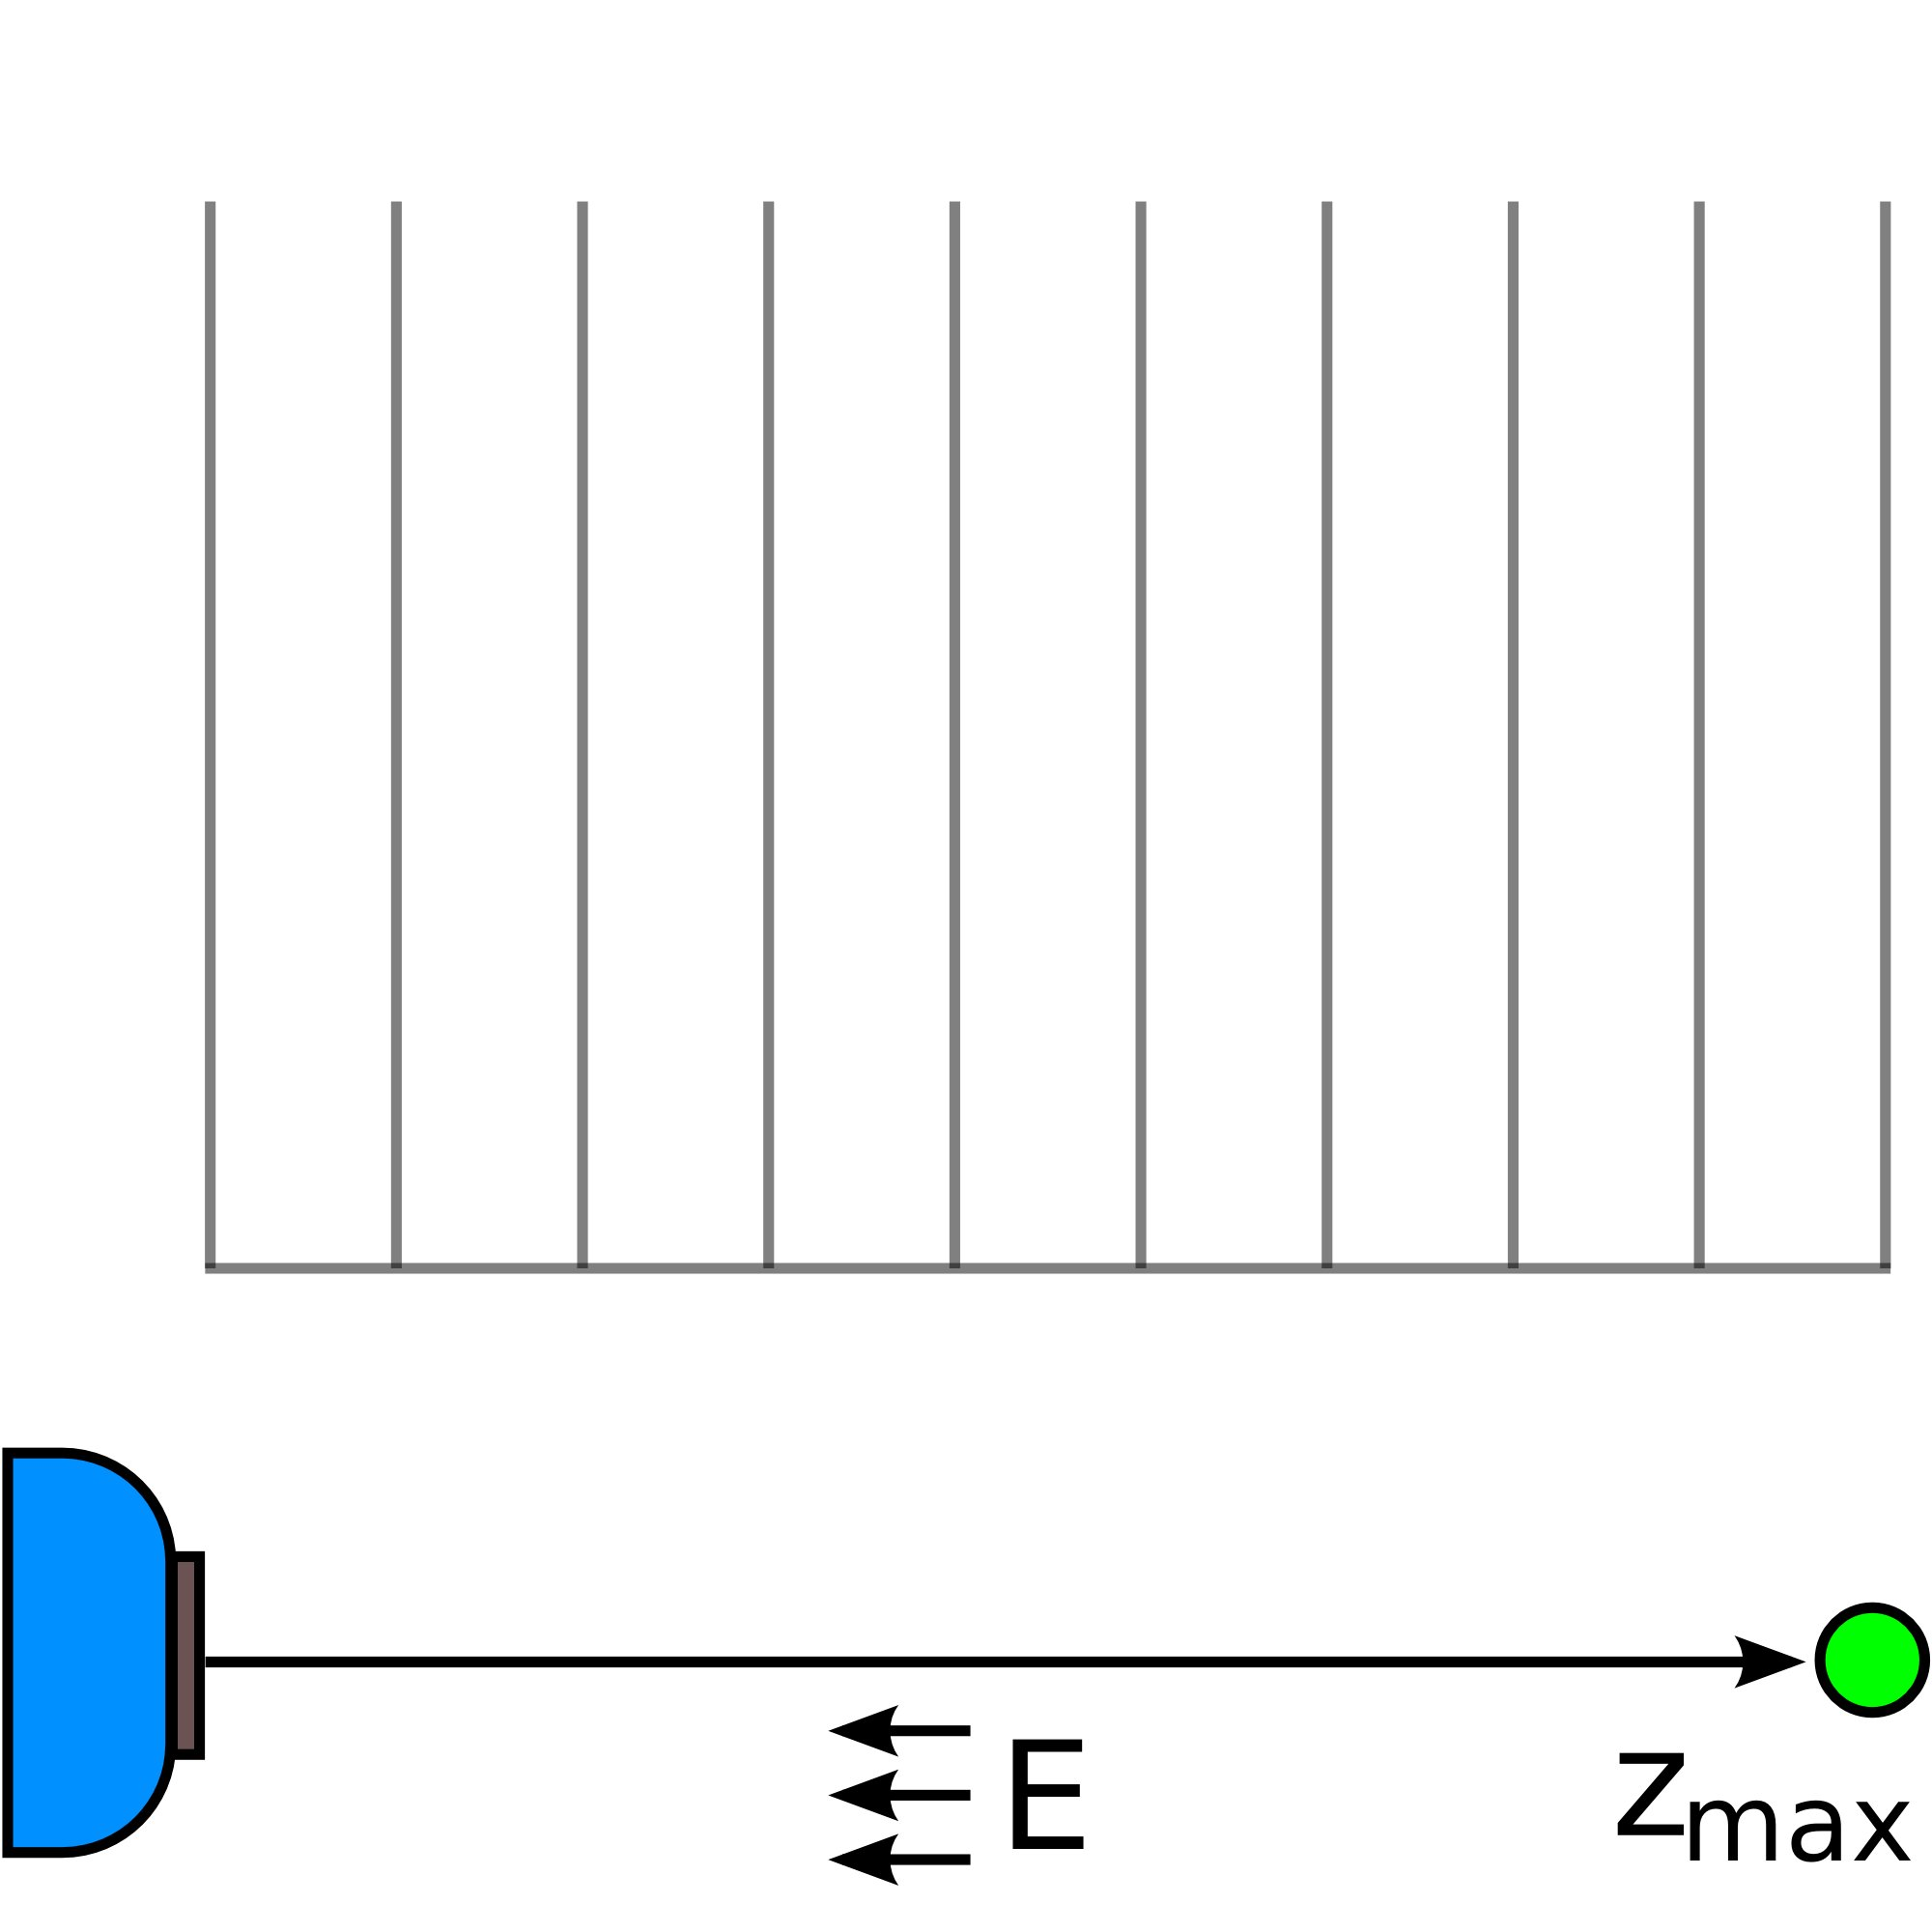
\includegraphics{bin2}}
    	\only<3>{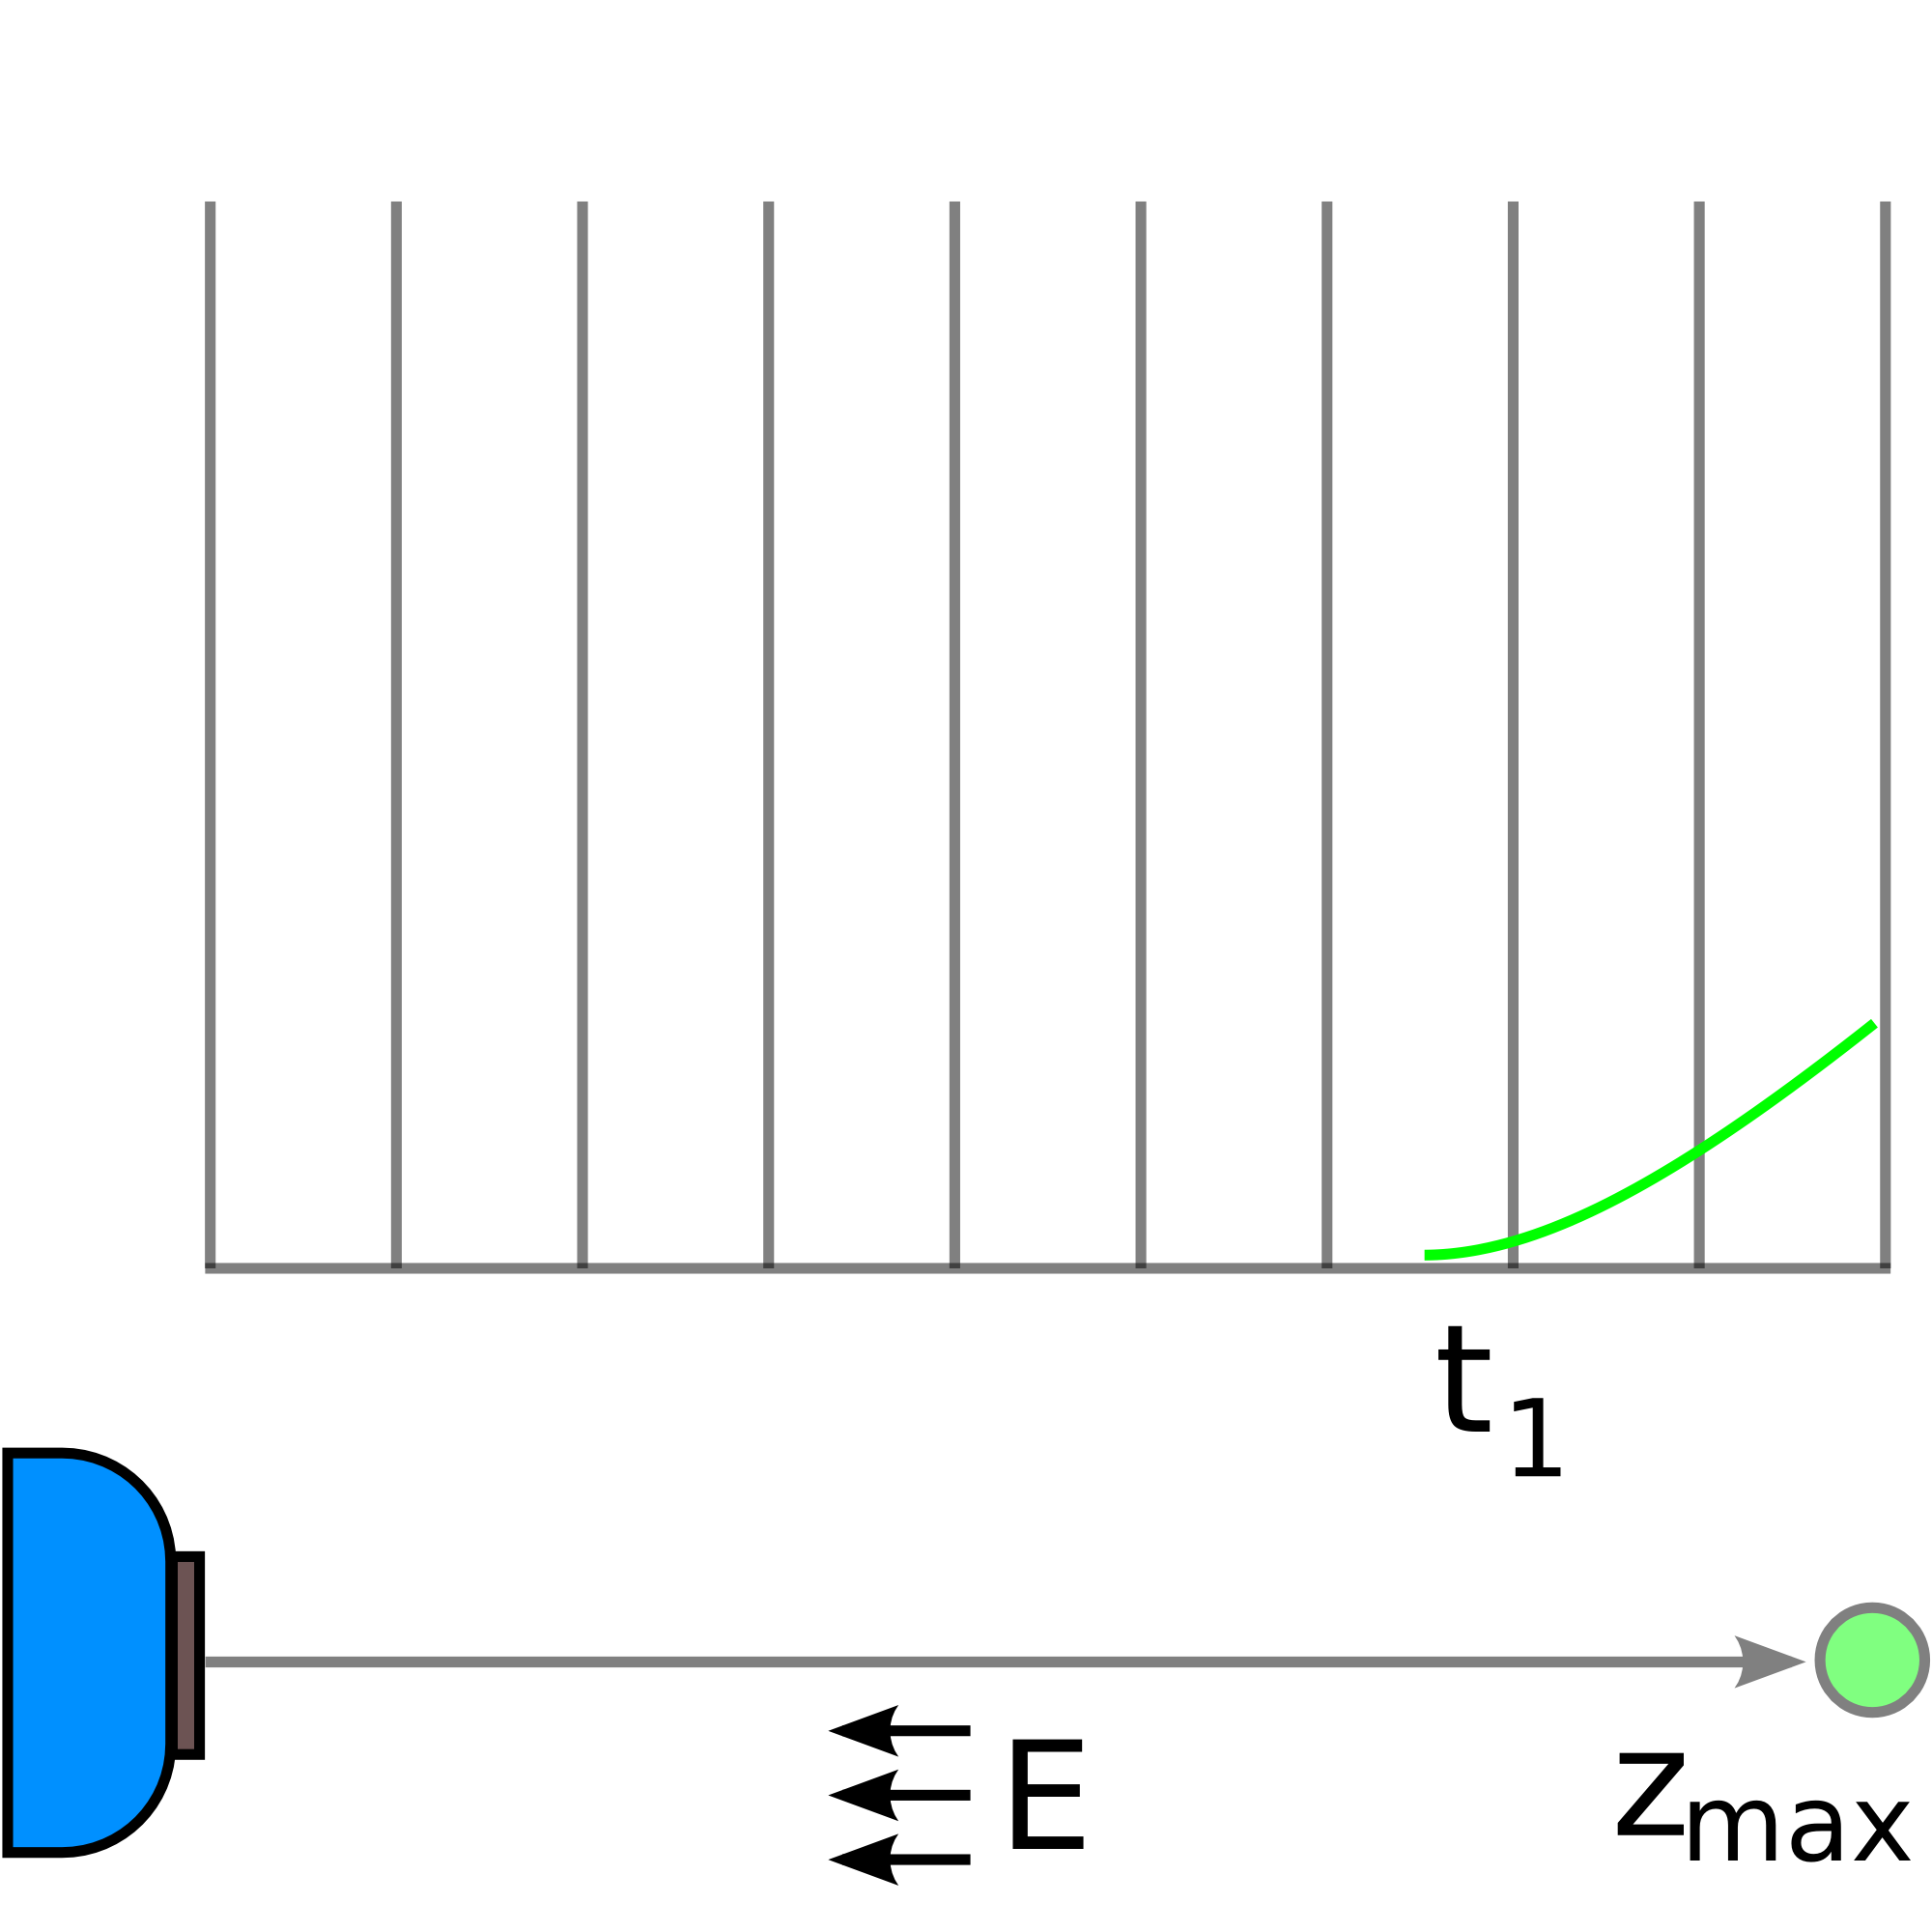
\includegraphics{bin3}}
   	    \only<4>{\includegraphics{bin4}}
    	\only<5>{\includegraphics{bin5}}
    	\only<6>{\includegraphics{bin6}}
    	\only<7>{\includegraphics{bin7}}
    	\only<8>{\includegraphics{bin8}}
    	}
    	\only<9->{\includegraphics{bin9}}
    	\only<article>
    	{
    	\caption{Overlay of time slices of distributions of electrons in space bins}
    	}
    \end{figure}
	\end{overlayarea}
	\end{column}
\end{columns}

\end{frame}

\begin{frame}{Comparison with Sipe Model}
\begin{columns}
	\begin{column}{3in}
	\begin{figure}[H]
    	\centering
		\includegraphics{Acc}
		\only<article>{\caption{Acceleration dominated case}}
	\end{figure}
	\end{column}

	\begin{column}{.38 \linewidth}
		\begin{block}{For operating conditions:}    
			$ qE/m >> v_{max}/t_{total} $
		\end{block}

		\vf
 
		\only<2->
		{
		For a majority of electrons the allowed fit is reasonable
		}

    \end{column}
\end{columns}
\end{frame}

\begin{frame}
\only<presentation>{\frametitle{Comparison with Sipe Model}}
\begin{columns}

	\begin{column}{.38 \linewidth}
		\begin{block}{For operating conditions:}    
			$ qE/m << v_{max}/t_{total} $
		\end{block}

		\vf
 
		\only<2->
		{
		In this case, the fit for ``local momentum width'' (related to
		$\eta$) not very good
		}

    \end{column}

	\begin{column}{3in}
	\begin{figure}[H]
    	\centering
		\includegraphics{Vmax}
		\only<article>{\caption{Vmax dominated case}}
	\end{figure}
	\end{column}

\end{columns}
\end{frame}

\begin{frame}
\only<presentation>{\frametitle{Comparison with Sipe Model}}
\begin{columns}
	\begin{column}{3in}
	\begin{figure}[H]
  		\centering
		\includegraphics{Equal}
		\only<article>{\caption{Case where Vmax and Acceleration are approximately equal}}
	\end{figure}
	\end{column}

	\begin{column}{.38\linewidth}
		\begin{block}{For operating conditions:}    
			$ qE/m \approx v_{max}/t_{total} $
		\end{block}

		\vf
 
		\only<2->
		{
		Even this more intermediate case will still have some artifacts
		owing to the limitations of the model
		}

    \end{column}
\end{columns}
\end{frame}

\begin{frame}{Regenerative Laser Amplifier}
  Regenerative laser amplifier:
  \begin{columns}
    \begin{column}{0.49\linewidth}
      \begin{itemize}
        \item 650Hz
        \item 100$\mu$J fundamental
        \item<2-> [$\hookrightarrow$] Generates $10^8$ electrons
        \begin{itemize}
          \item<3-> Single-shot imaging
          \item<4-> Observe charge-charge interaction
          \item<5-> Investigate short-pulse Child's Law
        \end{itemize}
      \end{itemize}
    \end{column}
    \begin{column}{0.49\linewidth}
    \begin{center}
      \includegraphics{regen}
    \end{center}
    \end{column}
  \end{columns}
\end{frame}


\end{document}
